\documentclass{book}

\usepackage{amsmath,amssymb,amsthm,subfigure,xcolor,graphicx,url}
\usepackage{fullpage}
\usepackage{alltt}

\usepackage{html}

\usepackage{hyperref}
\definecolor{linkcolour}{rgb}{0,0.2,0.6} % Link color
\hypersetup{colorlinks,breaklinks,urlcolor=linkcolour,linkcolor=linkcolour,citecolor=linkcolour} % Set link colors throughout the document

\usepackage{multind}
\makeindex{code}

\def\R{\mathbb{R}}

\def\tr#1{\mathrm{tr}\left(#1\right)}

\def\G{\mathcal{G}}

\newcommand{\red}[1]{\textcolor{red}{{#1}}}
\newcommand{\blue}[1]{\textcolor{blue}{{#1}}}
\definecolor{mygray}{HTML}{F8F9FA}


% Cool code that renders ' appear correctly in verbatim environment
\makeatletter
\let \@sverbatim \@verbatim
\def \@verbatim {\@sverbatim \verbatimplus}
{\catcode`'=13 \gdef \verbatimplus{\catcode`'=13 \chardef '=13 }} 
\makeatother


\title{Optimal Projections for Clustering: A MATLAB and GNU Octave package for Dimensionality Reduction for Clustering}
\author{Nicos G. Pavlidis}
\date{}

\def\mm#1{$#1$}

\begin{document}
\begin{htmlonly}
\def\href#1#2{\htmladdnormallink{#2}{#1}}
\def\mm#1{{\it #1}}
\end{htmlonly}

\maketitle
\tableofcontents

\chapter{Preface}

OPC is an open source MATLAB and GNU Octave package that implements dimensionality
reduction methods for clustering. 
%
This is a recognised problem in high-dimensional data
clustering~\cite{KriegelKZ2009}, but also occurs whenever irrelevant features,
or correlations among subsets of features exist. These characteristics, cause
the spatial data structure, which is inferred from pairwise distances, to be
less informative about the underlying clusters. To correctly identify cluster
structure, algorithms need to simultaneously solve two interrelated problems,
(a) identify the subspace in which clusters can be distinguished, and (b)
associate observations to clusters~\cite{KriegelKZ2009}.



OPC focuses on methods which seek low dimensional subspaces that are optimal
with respect to either a measure of clusterability, or of cluster separation.
%
This distinguishes this package from generic dimensionality reduction methods
%
\footnote{Numerous generic dimensionality reduction methods are implemented in
the \href{https://lvdmaaten.github.io/drtoolbox/}{MATLAB toolbox for
dimensionality reduction}.},
%
that determine the low dimensional data embedding by optimising an objective
function that is not related to any clustering criterion~\cite{MaatenPH2009}. 
%
Consequently, although some of these methods, most notably Principal Component
Analysis (PCA) have been
successfully applied in numerous applications, generic dimensionality
reductions method are not guaranteed to find a subspace that preserves (or
reveals) the cluster structure. 
%
A further limitation of these methods is that the low dimensional data embedding
typically varies substantially across different methods. This is a problem from
a user's perspective because there is no principled approach to select one
embedding over the others, even if user knows which type of clusters he/she is seeking.
%
%A generic dimensionality reduction methods, have been implemented in
%the MATLAB programming language~\cite{MaatenPH2009}.
%%
%%including the classical Principal Component Analysis, and Multi-Dimensional
%%Scaling, as well as more recently proposed algorithms like Isomap, Local
%%Linear Embedding, Laplacian Eigenmaps, and $t$--Distributed Stochastic
%%Neighbour Embedding
%%%
%%Although some of these methods, like Principal Component Analysis and
%%Multi-Dimensional Scaling, are widely used in clustering, 
%%
%These methods project the data onto a low dimensional space by 
%optimising an objective function that is not connected to any clustering
%criterion. Consequently, although some of these methods have been successfully
%applied in a plethora of applications, 
%none of these methods is guaranteed to find a subspace
%that preserves (or reveals) the cluster structure in the data.  In contrast OPC
%implements clustering algorithms that


To the best of our knowledge OPC is the only package in the MATLAB programming
language that implements dimensionality reduction methods explicitly designed
for clustering.
%
The methods included optimise clusterability criteria motivated from $k$-means,
normalised cut, spectral, and density clustering.
%
Partitioning, as well as divisive hierarchical clustering algorithms are
provided, with the latter being more appropriate to detect clusters defined in
different subspaces.
%
All the implemented algorithms require minimal input from the user, and employ
parameter settings recommended in the literature. However, the user can modify
all the parameters of each algorithm by specifying optional arguments.


A very appealing characteristic of clustering algorithms that perform dimensionality
reduction internally is that they enable the visualisation of the clustering
model. Such visualisations are crucial for the validation of a clustering
model, unless strong assumptions about the types of clusters are imposed. OPC
enables such visualisations, for all the algorithms it includes. The optimal
projection matrix is one of the outputs of all partitioning algorithms in the
package. This matrix jointly with the cluster assignment vector, can be readily
used to visualise the clusters.
%
The divisive hierarchical algorithms, return the cluster hierarchy as an object
of the cluster tree class, {\tt ctree}.
%
This class enables the visualisation of the binary partition at each
node of the cluster hierarchy (tree). 
%
%It also allows the user to modify the clustering model in 
%
It also enables the modification of the clustering model by pruning subtrees,
or partitioning leaves of the current model.
%
The binary partition at any node of the {\tt ctree} object can also be altered
by modifying the arguments of the projection pursuit algorithm used to produce
it. Examples of this are provided in Section~\ref{sec:valid}.


To render OPC extensible, we include an interface that allows the user to
create divisive hierarchical algorithms that have all the aforementioned
features by providing as input only a projection pursuit function for
clustering. Section~\ref{sec:extend} illustrates how to obtain the well known
bisecting $k$-means algorithm~\cite{SteinbachKK2000} through this approach.

%Finally, extensions to problems involving clusters which are not linearly separable and
%to the problem of finding maximum margin hyperplanes for clustering are also
%discussed.

%\clearpage

\chapter{Installation}


OPC depends on the following two packages, which are included in the package:

\begin{enumerate}

\item A cluster tree class, called {\tt ctree}\/, which is a
modification of the
\href{https://uk.mathworks.com/matlabcentral/fileexchange/35623-tree-data-structure-as-a-matlab-class}
{{\tt tree} class} by
Jean-Yves Tinevez.

\item The
\href{https://uk.mathworks.com/matlabcentral/fileexchange/17438-fast-gaussian-transform-mex-implementation}
{Fast Gauss Transform mex implementation} (FGT) by Sebastien Paris.

\end{enumerate}

\noindent
%
To install OPC a C and C++ compiler is required to compile FGT and two C++
functions used to compute one dimensional Gaussian kernel density estimators
and their derivative. Detailed instructions for the setup of the package in
MATLAB and Octave are provided in the following sections.


To create an online function reference for the package the 
%
\href{https://www.artefact.tk/software/matlab/m2html/}{M2HTML}
%
documentation system is required.


\section{MATLAB}

OPC requires the statistics and optimization MATLAB toolboxes. 

\subsubsection{Linux/ Mac}

We strongly suggest using the GNU Compiler Collection (GCC), that is readily
installed in both systems. To verify that {\tt mex} is correctly configured,
type in the MATLAB command line interface (CLI):

\begin{verbatim}
>> mex -setup
MEX configured to use 'gcc' for C language compilation.
\end{verbatim}


\begin{enumerate}

\item Once {\tt mex} is correctly configured the FGT and the C++ functions need to be
compiled. This needs to be performed only once. From the root directory of the
package execute the script:

\begin{verbatim}
>> mexme_fgt
\end{verbatim}

\item To use OPC after each MATLAB restart the path variable needs to be set to include
the root directory of the package and its sub-folders. 
For convenience, we provide the script {\tt setpath} (located in the root
directory of the package) to perform this task:

\begin{verbatim}
>> setpath
\end{verbatim}


\end{enumerate}

\subsection{Microsoft Windows}

A potential problem with setting up OPC in Windows is the lack of a C/C++ compiler which
can be used to compile the C code for the FGT, and two C++ functions which are
used to compute efficiently one dimensional Gaussian kernel density estimators
and their derivative. These need to be compiled once before the package is used
for the first time. 
%
To diagnose whether {\tt mex} is correctly configured on your system execute:

\begin{verbatim}
>> mex -setup
\end{verbatim}

\noindent
If the above command exits with an error:\\

\noindent
{\tt
Error using mex\\
No supported compiler or SDK was found.}\\

\noindent
{\tt mex} is not configured to use a C/C++ compiler.
%
Refer to this \href{https://uk.mathworks.com/support/compilers.html}{link} for
a list of compilers supported by MATLAB R2018a.
We next provide instructions for how to install the {\tt MinGW-w64} compiler which
can be used on the current as well as previous releases of MATLAB.


\subsubsection{Installing MinGW-w64 compiler in Windows}

Mathworks provides instructions to
\href{https://uk.mathworks.com/help/releases/R2015b/matlab/matlab_external/install-mingw-support-package.html}
{install the MinGW-w64 compiler from the add-ons menu}.
%
If this is unsuccessful you can install this compiler manually by following the steps below:

\begin{enumerate}

\item Download the TDM-GCC MinGW installer, from this \href{https://sourceforge.net/projects/tdm-gcc/}{SourceForge}.
%Although MATLAB 
%\href{https://uk.mathworks.com/matlabcentral/fileexchange/52848-matlab-support-for-mingw-w64-c-c++-compiler}
%{installs older version of this compiler for different distributions},
%I manually installed the most recent version, 5.1.0-2, from
%\href{https://sourceforge.net/projects/tdm-gcc/}{SourceForge} and set up the mex to use it successfully.


\item Run the TDM-GCC MinGW installer and disable the option ``Check for
updated files on the TDM-GCC server" that appears on the first screen,
\href{https://uk.mathworks.com/help/releases/R2015b/matlab/matlab_external/install-mingw-support-package.html}
{as suggested by Mathworks}.

\item In the first screen of the installer select ``Create'' to create a new
installation and ensure that you install the compiler in a directory like:\\
{\tt C:\char`\\TDM-GCC-64}\\
and not in ``Program Files" or any directory whose path contains spaces, 
\href{https://uk.mathworks.com/help/releases/R2015b/matlab/matlab_external/install-mingw-support-package.html}
{as suggested by Mathworks}.

\item After completing the installation of TDM-GCC MinGW, MATLAB will still be
unable to find the MingGW-w64 compiler because the environment variable
{\tt MW\_MINGW64\_LOC}
is not defined.
Use the {\tt setenv()} command to set this variable:

\begin{verbatim}
>> setenv('MW_MINGW64_LOC','C:\TDM-GCC-64')
>> mex -setup
MEX configured to use 'MinGW64 Compiler (C)' for C language compilation.
\end{verbatim}

The output message in the last line above verifies that {\tt mex} is correctly configured.
For our purposes setting up the {\tt mex} compiler once is sufficient as the FGT package
and the other C++ functions needs to be compiled only once. Bear in mind
however that if you need to use {\tt mex} again
you need to set this environment variable after every restart of MATLAB.

\end{enumerate}

Having configured {\tt mex} correctly, we can compile all the C and C++ code.
Recall that this needs to be done only once. 
From the root directory of OPC execute:

\begin{verbatim}
>> mexme_fgt
\end{verbatim}

\noindent Finally, after each restart of MATLAB the current directory and all
its subfolders need to be included in its path. For convenience, we provide the
script {\tt setpath} located in the root directory of the package to do this:

\begin{verbatim}
>> setpath
\end{verbatim}


\section{GNU Octave}

OPC uses object oriented programming and in particular contains {\tt classdef}
classes. These are only supported after the
\href{https://octave.org/doc/v4.2.2/classdef-Classes.html#classdef-Classes}
{GNU Octave 4.0} release. The
following list enumerates the requirements and necessary steps to install OPC in
Octave:

\begin{enumerate}

\item OPC requires
the statistics package, and the non-linear optimization package, optim. Both
packages can be found at the
\href{https://octave.sourceforge.io/packages.php}{extra packages for GNU
Octave} repository.
%
Detailed instructions to install and load extra packages in Octave are provided in
relevant
\href{https://octave.org/doc/interpreter/Packages.html#Packages}{documentation} page.

\item The C implementation of the Fast Gauss Transform, as well as two
C++ functions necessary to efficiently compute one dimensional Gaussian kernel density
estimators and their derivatives, need to be compiled before the package
is used for the first time. For this purpose a C/C++ compiler is required. 
We recommend using the GNU Compiler Collection (GCC). 
%
To verify the configuration of the {\tt mex} compiler execute the following:

\begin{verbatim}
>> mex --print CC
>> mex --print CXX
\end{verbatim}

\noindent
To compile FGT and the C++ functions, execute from the root directory of the
package the script:

\begin{verbatim}
>> mexme_fgt
\end{verbatim}

\item To use OPC after each Octave restart the path variable needs to be set to include
the root directory of the package and its sub-folders. 
For convenience, we provide the script {\tt setpath} (located in the root
directory of the package) to perform this task:

\begin{verbatim}
>> setpath
\end{verbatim}

\end{enumerate}


\section{Documentation}


The source code ({\TeX} file and all the necessary PNG figures) to compile this document is
provided in the directory {\tt documentation}. (All directories in this
document are relative to the root directory of the OPC package). This
directory also contains the compiled, PDF, version of this document.
%
An HTML version of the documentation can be readily created using
\href{http://www.latex2html.org/}{LaTeX2HTML}.
%
We recommend using LaTeX2HTML with the following parameters:

\begin{verbatim}
[user@host:documentation]$ latex2html -split 4 -white document.tex
\end{verbatim}



The script file {\tt reproduction\_script.m} in the root OPC directory
contains all the material to reproduce every example in this
document. To recreate all the figures (in PNG format) uncomment the
lines which call the {\tt print} function, which follow 
calls to the 
{\tt plot} and {\tt nplot} functions. Beware that the new figures
will be stored in the {\tt documentation/figures} directory,
overwriting the existing figures there.


\subsection{HTML Function Reference}

The
%
\href{https://www.artefact.tk/software/matlab/m2html/}{M2HTML}
%
documentation tool can be used to automatically generate an HTML function
reference for OPC.  To create this follow the steps below:

\begin{enumerate}

\item Download the M2HTML from:
%
\url{https://www.artefact.tk/software/matlab/m2html/}

Uncompressed the zip file in a folder of your choice, e.g.
{\tt /home/user/Downloads}.

\item From the root directory of the OPC package copy the folder
{\tt documentation/m2html\_template/docs} 
%
to the M2HTML folder {\tt templates} folder
{\tt /home/user/Downloads/m2html/templates}


\item From MATLAB or Octave, add the M2HTML folder to the path;
configure the path for the OPC package, and execute
the script {\tt create\_reference}:

\begin{verbatim}
>> % From root OPC directory: add OPC folders to path 
>> setpath
>> % Add m2html folder to path
>> addpath('/home/user/Downloads/m2html');
>> % Create HTML function reference
>> create_reference
\end{verbatim}

\end{enumerate}

\noindent
%
The HTML function reference is located in the directory {\tt
documentation/reference}.  To access it use a web-browser to open the file {\tt
index.html} located in this directory.



%\clearpage

%\section{A Brief Introduction to OPC}

\chapter{Implemented Methods}

The OPC package contains implementations of the following clustering
algorithms:

\begin{enumerate}

\item Principal Direction Divisive Partitioning (PDDP)~\cite{Boley1998}

\item Density-enhanced Principal Direction Divisive Partitioning (dePDDP)~\cite{TasoulisTP2010}

\item Minimum Density Divisive Clustering~(MDDC)~\cite{PavlidisHT2016}

\item Maximum Clusterability Divisive Clustering~(MCDC)~\cite{HofmeyrP2015}

\item Linear Discriminant Analysis $k$-means (LDA-$k$-means)~\cite{DingL2007}

\item Dimensionality Reduction for Spectral Clustering (DRSC)~\cite{NiuDJ2011,NiuDJ2014}

\item Minimum Spectral Connectivity Projection Pursuit (SCPPDC)~\cite{HofmeyrPE2018}

\item Minimum Normalised Cut Divisive Clustering~(NCUTDC)~\cite{Hofmeyr2017}

\item Bisecting $k$-means~\cite{SteinbachKK2000} (the implementation of this
algorithm is used as an illustration of how the user can extend the package)

\end{enumerate}


\noindent
In the following brief exposition of the implemented methods we assume that
the dataset is stored in the data matrix consists of $n$ vectors
in $d$-dimensional Euclidean space, stored in the data matrix $X \in \mathbb{R}^{n \times d}$. 

\section{Principal Direction Divisive Partitioning and density-enhanced version}

The most widely used approach to combine dimensionality reduction and
clustering is to project the $d$ dimensional dataset onto the first~$q$ principal components. 
%
Principal Component Analysis (PCA) can be considered the most popular projection
pursuit method. PCA can be formulated either as maximising the variance of the
projected data, or minimising the squared reconstruction
error~\cite{Jolliffe1986}. PCA is the only projection pursuit method that has
a closed form solution. For a given choice of $q$, the projection index is
optimised by the $q$ eigenvectors associated with the $q$ largest eigenvalues
of the data covariance matrix.
%
Although there is no guarantee that the subspace spanned by any $q<d$
principal components preserves cluster structure, this approach has been found
to work well in a number of applications~\cite{KriegelKZ2009}.

PDDP and dePDDP and are two divisive clustering algorithms that recursively
project (subsets of) the data onto the first principal component.
PDDP bi-partitions the data by splitting at the mean of the projections, while
dePDDP constructs a one-dimensional kernel density estimator (KDE) and splits
at lowest local minimum.
%
Effectively, both algorithms bi-partition each cluster 
using a separating hyperplane,
\[
H(v,b) = \{x \in \R^d \,|\, v^\top x= b\},
\]
where $v \in \mathbb{S}^{d} = \{ x \in \R^d \,|\, x^\top x=1\}$ is the
vector normal to the separating hyperplane,
and $b \in \R$ is the displacement of the separating hyperplane from the origin.


\section{Minimum Density Divisive Clustering}

The Minimum Density Divisive Clustering (MDDC) algorithm recursively
bi-partitions the data using Minimum Density
Hyperplanes~(MDHs)~\cite{PavlidisHT2016}. An MDH
avoids intersecting high density clusters by seeking the hyperplane
that minimises the integral of the empirical probability density function along
its surface,
%
\[
\hat{I}(v,b) = \int_{ H(v,b)} \hat{p}(x) \mathrm{d} x.
\]
%
If a density estimator that uses isotropic Gaussian kernels is employed,
%
\[
\hat{p}(x) = \frac{1}{n (2 \pi h^2)^{d/2} } \sum_{i=1}^n \exp \left\{ -\frac{ \|x - x_i \|^2}{2 h^2} \right\},
\]
%
then $\hat{I}(v,b)$ can be estimated from the one-dimensional data projection,
%
\[
\hat{I}(v,b) = \frac{1}{n\sqrt{2\pi h^2 }} \sum_{i=1}^n  \exp \left\{- \frac{ (b - v^\top x_i)^2 }{2 h^2} \right\}.
\]
%
The ability to compute $\hat{I}(v,b)$ through the above equation enables us to
estimate MDHs. MDH is the solution to the following optimisation problem,
%
\begin{align}
%
v^\star & = \min_{v \in \mathbb{S}^d} f(v), \label{eq:mdh1} \\
%
f(v) & = \min_{b \in \R} \left\{ \hat{I}(v,b) + c_0 \max \left\{0, \mu_v  -\alpha
\sigma_v - b, b - \mu_v  -\alpha \sigma_v \right\}^{1+c_1} \right\}, \label{eq:mdh2}
%
\end{align}
%
The second term in the last equation, $c_0 \max \left\{0, \mu_v  -\alpha
\sigma_v - b, b - \mu_v  -\alpha \sigma_v \right\}^{1+c_1}$,
is a penalty function that ensures that
the optimal MDH is within $\alpha$ standard deviations, $\sigma_v$ from the mean of the
projected data, $\mu_v$. Such a constraint is necessary since it is always possible
to obtain hyperplanes with density arbitrarily close to zero if the hyperplane is sufficiently
far from the centre of the data.
%
The terms $c_0$ and $c_1$ are constants whose values are fixed (see~\cite{PavlidisHT2016}),
while $\alpha$ is adaptively set by the projection pursuit algorithm.


The most computationally expensive task in the estimation of MDHs is the minimisation of
the one dimensional kernel density estimator, for each $v$.
This is achieved by first evaluating $f(v)$ on a grid of $m$ points, to bracket the location
of the minimiser, and then applying bisection to compute the minimiser
at the desired accuracy.
%
The Fast Gauss Transform~\cite{Morariu08} reduces the computational
cost of the first step, and by far most computationally expensive step,
from $\mathcal{O}(mn)$ to $\mathcal{O}(m+n)$. Bisection requires $\mathcal{O}(-\log_2
\varepsilon)$ iterations to locate the minimiser with accuracy~$\varepsilon$.


\section{Maximum Clusterability Divisive Clustering}

The variance ratio clusterability~\cite{Zhang2001} is a measure of strength or conclusiveness
of the cluster structure in a dataset. 
%
Let $\{C_i\}_{i=1}^k$ denote a $k$-way partition of the dataset $X$, and $\{m_i\}_{i=1}^k$
the centroids of each of the $k$~clusters. Then the variance ratio clusterability of~$X$ is defined
as,
%
\begin{align*}
%
& \max_{C_1,\ldots,C_k}\frac{\sum_{j=1}^k |C_j| \,  \|m_j - m\|^2}
	{\sum_{j=1}^k   \sum_{x_i \in C_j}\|x_i - m_j\|^2},\\
%
\text{such that: } & X = \bigcup_{i=1}^k  C_i, \text{ and }  C_i \cap C_j = \emptyset, \forall i \neq j.
%
\end{align*}
%
It is easy to show that the partition that maximises Variance Ratio clusterability
also minimises the $k$-means objective function,
%
\begin{align*}
%
& \min_{C_1, \ldots, C_k} \sum_{i=1}^n \min_{j = 1, \dots, k}\|x_i - m_j\|^2,\\
%
\text{such that: } & X = \bigcup_{i=1}^k  C_i, \text{ and }  C_i \cap C_j = \emptyset, \forall i \neq j.
%
\end{align*}
%

The Maximum Clusterability Divisive Clustering (MCDC)~\cite{HofmeyrP2015}
algorithm recursively bi-partitions the data using hyperplanes, $H(v,b)$, that maximise
the variance ratio clusterability index of the binary partition of the data projected onto $v$. 
%
Such hyperplanes are called Maximum Clusterability Hyperplanes (MCHs). 
%
For any $C \subsetneq X$ the binary partition of $X$ is given by $\{C, X \setminus C\}$.
Let $\mu, \mu_{C}$ and $\mu_{X\setminus C}$ be the
means of $X, C$ and $X\setminus C$ respectively, and 
$\Sigma$ the data covariance matrix, $\Sigma = n^{-1} \sum_{i=1}^n (x_i - \mu)(x_i-\mu)^\top$.
%
Then the projection index for a given~$v$ is given by,
%
\begin{align*}
%
f(v) = \max_{C \subset X} \frac{\vert C | \left(v^\top( \mu_{C} - \mu)\right)^2 + (n-|C|)\left(v^\top( \mu_{X \setminus C} - \mu)\right)^2}{\frac{n}{n-1}v^\top \Sigma v +   \sum_{x_i \in C}\left(v^\top(x_i - \mu_{C})\right)^2 +  \sum_{x_i \in X\setminus C}\left(v^\top(x_i - \mu_{X \setminus C})\right)^2}.
%
\end{align*}
%
For the special case of one dimensional data it is possible to identify the set $C^\star$
that optimises the variance ratio clusterability in 
$\mathcal{O}(n \log n)$ time. This is feasible because in this case the set $C^\star$ 
satisfies, $C^\star = \{ x \in X \,|\, v^\top x < b \}$ for some
$b \in \R$.


\section{Linear Discriminant Analysis {\it k}--Means}\label{sec:ldakmeans}

The LDA-$k$-means algorithm~\cite{DingL2007} exploits the connection between
Linear Discriminant Analysis (LDA) and $k$-means clustering. To see 
this we first need to introduce some notation.
%
Without loss of generality assume that the data is centred at zero.
%
Define the total scatter, the between-cluster scatter, and the within-cluster
scatter matrices as,
\begin{align*}
%
S_t & = \sum_{i=1}^n x_i x_i^\top, \\
%
S_b & = \sum_{j=1}^k n_j m_j x_j^\top, \\
%
S_w & = \sum_{j=1}^k \sum_{x_i \in C_j} (x_i - m_j)(x_i - m_j)^\top.
%
\end{align*}
%
Then the $k$-means objective function can be expressed as,
%
\[
\min_{C_1,\ldots,C_k} \sum_{j=1}^k \sum_{x_i \in C_j} \|x_i - m_j\|^2 = \min_{C_1,\ldots,C_k} \tr{S_w},
\]
where $\tr{\cdot}$ is the trace operator. Since $S_t = S_w + S_b$, minimising
$\tr{S_w}$ is equivalent to maximising $\tr{S_b}$.

In LDA the cluster assignment (class labels) are assumed known and the
algorithm seeks the orthonormal matrix $U \in \R^{d \times k}$ that,
%
\[
%
\max_{U} \frac{ \tr{U^\top S_b U}}{\tr{U^\top S_w U}}, \; \text{ s.t. } \; U^\top U = I.
%
\]

The fact that both LDA and $k$-means aim to minimise the within cluster (class)
scatter and maximise the between class scatter motivates the LDA-$k$-means
algorithm. 
%
LDA-$k$-means is a two step iterative algorithm. In the first step the
$(k-1)$-dimensional linear subspace in which the data is projected is
fixed, and the objective is to identify the cluster assignment that maximises
the ratio of the between class scatter to the within class scatter:
%
\begin{equation}\label{eq:ldakm}
%
\max_{C_1,\ldots,C_k} \frac{\tr{U^\top S_b U}}{\tr{U^\top S_w U}}.
%
\end{equation}
%
The $k$-means algorithm is applied to obtain the solution to this problem.
%
In the second step the cluster (class) assignment is considered fixed and
the objective is to identify the orthonormal matrix~$U$ that maximises
the objective function. For a fixed cluster assignment, LDA provides a closed
form solution to this problem. The only element of the algorithm that remains
unspecified is the specification of $U$ at the first step. In~\cite{DingL2007} it is
recommended to initialise~$U$ to the first $(k-1)$~principal components.

It is important to note that the LDA-$k$-means algorithm is not 
guaranteed to converge, or even to to
monotonically improve the objective function,~Eq.~(\ref{eq:ldakm}). 
%
As is well-known the $k$-means algorithm is not guaranteed to identify the globally
optimal solution, and even if that were the case it is not clear that
the proposed two-stage procedure would be globally convergent.
%
%From an implementation perspective, the initialisation of $k$-means 
%in MATLAB and Octave (but also in other languages) involves randomisation and consequently
%the output of the {\tt kmeans} function differs over executions.
%This can cause produce very different results for LDA-$k$-means.

\section{Introduction to Normalised Graph Cuts and Spectral Clustering}

The approach to clustering based on graph theory associates clusters with strongly
connected components of a graph, $\G = (V,E)$\/. The set vertices, $V$ corresponds
to the data points, $V=X$, while edge weights, $E_{ij}$ represent pairwise
similarities between them~\cite{Luxburg2007}.
%
The graph, $\G$, can be equivalently represented through an adjacency, or similarity, matrix, $A \in
\R^{n \times n}$, defined as,
%
\[
A_{ij} = k(x_i, x_j),
\]
%
where $k(\cdot)$ is a kernel function, most typically the Gaussian kernel.
%
The degree of a vertex is defined as,
%
\[ d_i = \sum_{j=1}^N A_{ij}.\]
%
%
For any subset $C \subset X$, 
%
%the size of $C$ can be measured either by its cardinality, $|C|$, or by its volume
%
the volume of $C$ is defined as:
%
\[ \textrm{vol}(C) = \sum_{x_i \in C} d_i.\]
%

A graph cut is a partition of the vertices of a graph into $k$ pairwise
disjoint components. The \emph{normalised cut} of a graph is the
solution to the following optimisation problem,
%
\begin{equation}\label{eq:ncut}
%
\min_{C_1,\ldots, C_k} \textrm{NCut}(C_1,\ldots,C_k) = \min \sum_{j=1}^k \frac{\mathrm{cut}\left(C_j, X \setminus
C_j \right)}{\textrm{vol}(C_j)}, 
%
\end{equation}
where,
\begin{equation*}
\mathrm{cut}\left(C_j, X \setminus C_j \right) = \frac{1}{2} 
\sum_{j:\, x_j \in C_j} \sum_{i:\, x_i \in X\setminus C_j} A_{ji}
%
\end{equation*}
%
The normalisation by dividing the value of the cut,
$\mathrm{cut}\left(C_j, X \setminus C_j \right)$, with the cluster volume was
first proposed in~\cite{ShiM2000}. This normalisation discourages the optimal
solution from containing partitions with very few vertices/ data points, which
is undesirable a clustering perspective.
%
However, it also renders the problem NP-hard. 


Spectral clustering is a family of methods that solve a continuous relaxation
of the original NP-hard graph cut problem in (\ref{eq:ncut})~\cite{HagenK1992,ShiM2000,Luxburg2007}. 
%
To describe this approach for the normalised graph cut problem it is first necessary to
define the \emph{graph Laplacian} matrix:
%
\begin{align*}
%
L_n &= I - D^{-1/2}AD^{-1/2},
%
\end{align*} 
where $A$ is the adjacency matrix,
$D = \textrm{diag}(d_1,\ldots,d_n)$ is degree matrix, and $I$ is the identity matrix.
%
For a given $k$-way partition of $X$ into $\{C_1,\ldots,C_k\}$, define the matrix $(n \times k)$ matrix
$T$ as:
%
\begin{equation}\label{eq:spectralH}
%
T_{ij} = \left\{ \begin{array}{ll} \sqrt{d_i/ \mathrm{vol}(C_j)}, & \textrm{ if } x_i \in C_j, \\
	0, & \textrm{ otherwise}. \end{array} \right.
%
\end{equation}
The normalised minimum cut problem can be formulated as~\cite{ShiM2000}:
%
\[
%
\min_{C_1,\ldots,C_k} \tr{T^\top L_n T}, \; \textrm{ subject to: } T^\top T = I, 
	\textrm{ and } T \textrm{ as defined as in Eq.~(\ref{eq:spectralH})},
%
\]
%
or equivalently~\cite{NgJW2001}:
\[
%
\max_{C_1,\ldots,C_k} \tr{T^\top D^{-1/2} A D^{-1/2} T} \; \textrm{ subject to: } T^\top T = I,
	\textrm{ and } T \textrm{ as defined as in Eq.~(\ref{eq:spectralH})}.
%
\]
%
The continuous relaxation which gives rise to spectral clustering 
allows $T$ to
be any matrix in $\R^{n \times k}$~\cite{Luxburg2007}. 
The normalised cut spectral clustering problem is thus expressed as~\cite{ShiM2000}:
\[
\min_{T \in \R^{n \times k}} \tr{T^\top L_n T}, \; \textrm{ subject to: } T^\top T = I.
\]
The solution to the above optimisation problem is the matrix $T$ whose columns 
are the $k$~eigenvectors of~$L_n$ that correspond to the $k$ smallest
eigenvalues (or equivalently the $k$ eigenvectors that correspond to the $k$ largest
eigenvalues of $D^{-1/2} A D^{-1/2}$).
%
Since the complexity of computing a single eigenvector is $\mathcal{O}(n^2)$ the complexity
of spectral clustering algorithms is $\mathcal{O}(k n^2)$.



\section{Minimum Normalised Cut Hyperplanes (NCUTDC)}

In this section we briefly introduce a method that identifies optimal
hyperplanes for clustering based on the normalised graph cut criterion in
log-linear time~\cite{Hofmeyr2017}. Minimum Normalised Cut Divisive Clustering
(NCUTDC) relies on the fact that if the data is projected into one dimension
and the Laplace kernel is used to compute the pairwise similarities, 
%
\[A_{ij} = \exp\left( -\left|v^\top x_i - v^\top x_j\right|/\sigma \right) \]
%
then the binary partition $\{ C^\star, X \setminus C^\star\}$ that optimises
the normalised cut criterion for the projected data satisfies, $C^\star = \{x
\in X \,|\, v^\top x < b\}$ for some $b \in \R$. Therefore, the
optimal bi-partition can be identified by sorting the projected data,
$\mathcal{O}(n \log n)$ and then estimating the value of the normalised cut criterion
at $n$ points, $\mathcal{O}(n)$. The computational complexity
is therefore log-linear~\cite{Hofmeyr2017}.
%
The projection index for this method is:
%
\begin{align*}
%
f(v) & = \min_{b \in \R} \mathrm{NCut}\left( C_{v,b},  C_{v,b}^c \right), \;
\textrm{where},\\
%
C_{v,b} & = \{ v^\top x \,|\, v^\top x < b, x \in X\}, \\
%
C^c_{v,b} & = \{ v^\top x \,|\, v^\top x > b, x \in X\}, \\
%
\end{align*}

It is important to stress that because the projection index underlying NCUTDC
uses similarities computed on the projected data, this algorithm cannot operate
on an arbitrary graph or similarity matrix.

\section{Dimensionality Reduction for Spectral Clustering (DRSC)}

The Dimension Reduction Spectral Clustering (DRSC)~\cite{NiuDJ2011} algorithm
aims to identify the projection matrix, $V$, that maximises
the sum of the first $k$ eigenvalues of the $D^{-1/2}AD^{-1/2}$,
where both the similarity and degree matrices, $A$ and $D$ respectively,
are computed from the projected data, $XV \in \R^{n \times q}$.
%
The sum of the $k$ largest eigenvalues of $D^{-1/2}AD^{-1/2}$ is a measure of
spectral separability, with larger values indicating more separable clusters.
%
%\begin{subequations}\label{eq:DRSC}
%
\begin{eqnarray}
%
\max_{U, V} &  \mbox{trace}(U^\top D^{-1/2}AD^{-1/2}U), \label{eq:drsc1}\\
%	
\mathrm{s.t.} & U^\top U = I,\\
%
& A_{ij} = k(\|V^\top x_i - V^\top x_j \|), \label{eq:Aij}\\
%
&V^\top V = I.
%
\end{eqnarray}
%
%\end{subequations}
%
The above formulation is equivalent to minimising the sum of the 
$k$~smallest eigenvalues of~$L_n$.
%
It is clear that
for a given $V$ the matrix $U$ that maximises the trace in (\ref{eq:drsc1}) has
columns given by the~$k$ eigenvectors associated with the $k$~largest
eigenvalues of $D^{-1/2}AD^{-1/2}$ (or equivalently the $k$~smallest
eigenvalues of~$L_n$).
%%

DRSC proposes to solve the above optimisation problem by a two-stage algorithm.
In the first stage $V$ is fixed and the $k$ eigenvectors of $D^{-1/2}AD^{-1/2}$
are computed to estimate the optimal~$U$. In the second stage, $U$~is fixed and
for each column of $V$ gradient ascent is performed to maximise the trace
in~(\ref{eq:drsc1}). The projection index for this method can therefore be written as:
%
\begin{align*}
%
f(V) & = \sum^n_{n-k+1} \lambda_j \left( D^{-1/2}AD^{-1/2} \right) = \sum_{j=1}^k \lambda_j \left( L_n \right),\\
%
\textrm{ s.t. } & A_{ij} = k(\|V^\top x_i - V^\top x_j \|),\\
%
 & V^\top V = I,
\end{align*}
%
where $\lambda_j(\cdot)$ denotes the $j$-th smallest eigenvalue of 
its matrix argument.
%
However, in the computation of the gradient of $f(V)$ in the second stage of
the algorithm, the degree matrix $D$ is considered fixed, and therefore the
influence of~$V$ on the degrees of the vertices is ignored. Consequently, the
gradient estimated by assuming a fixed $D$, is not the gradient of the overall
objective function. There is no guarantee that this gradient is even an ascent
direction for the objective function.  This can cause this algorithm to fail to
converge.


\section{Spectral Connectivity Projection Pursuit Divisive Clustering (SCPPDC)}

The Spectral Connectivity Projection Pursuit Divisive Clustering
(SCPPDC)~\cite{HofmeyrPE2018} recursively bi-partitions the data by projecting
onto the linear subspace that minimises the second smallest eigenvalue of the
normalised graph Laplacian~$L_n$. 
%
In more detail, for each projection matrix, $V$, the data is first projected
onto $V$, and then the similarity, the degree and the normalised graph
Laplacian matrices are computed from the projected data.
%
The projection index employed by this method is the value of the second
smallest eigenvalue of $L_n(V)$ is the 
%
\[ f(V) = \lambda_2 \left(L_n(V) \right) + \omega V^\top V \]
%
Therefore, SCPPDC employs the same objective function as DRSC for the case when~$k=2$.
However, unlike DRSC, the projection pursuit algorithm employed by
SCPPDC is globally convergent because the algorithm uses the gradient of the
overall objective function. Furthermore in each gradient descent step SCPPDC
updates the entire projection matrix, rather than optimising each column of $V$
separately as in DRSC. 


\section{Bisecting {\it k}--means}

Bisecting $k$-means~\cite{SteinbachKK2000} is a well known divisive clustering
algorithm originally proposed for document clustering, that recursively applies
$2$-means. Since 2-means can be viewed as separating the clusters by first
projecting the data onto the vector connecting the two centroids and then
assigning observations to clusters based on their location relative to the
mid-point between the two centroids,
%
%a hyperplane whose normal vector is equal to the difference between the two
%centroids, 
%
this algorithm can be considered as performing dimensionality reduction.

Bisecting $k$-means is included in the package as an example of how a user can
extend the functionality of the package by specifying a function that performs
projection pursuit for clustering.


%\clearpage

%\section{General Information about OPC}

%\subsection*{General Syntax}
%
%The data matrix and the number of clusters are the only {\bf mandatory inputs} to all the
%algorithms, except for dePDDP, which can estimate the number of clusters
%automatically.
%%
%The only algorithm that requires an additional mandatory input is {\tt drsc}.
%No default setting for the scale parameter of the Gaussian kernel used to
%estimate the similarity/ kernel matrix is suggested in the literature, and thus
%this parameter needs to be explicitly set by the user.
%
%
%\subsubsection*{Output Arguments}
%
%The partitioning algorithms, {\tt ldakmeans} and {\tt drsc}, return as the
%first three output arguments:
%%
%\begin{itemize}
%
%\item[] {\tt idx}: A vector of cluster assignments, {\tt idx}~$\in \{1,\ldots,k\}^n$
%
%\item[] {\tt V}: The projection matrix
%
%\item[] {\tt fval}: The value of the projection index at termination 
%
%\end{itemize}
%%
%Both {\tt ldakmeans} and {\tt drsc} return additional output arguments that are
%specific to each algorithm.
%
%All divisive clustering algorithms in OPC return two output arguments:
%%
%\begin{itemize}
%
%\item[] {\tt idx}: A vector of cluster assignments, {\tt idx}~$\in \{1,\ldots,k\}^n$
%
%\item[] {\tt t}: A {\tt ctree} object that represents the cluster hierarchy
%
%\end{itemize}
%
%
%\subsubsection*{Main Optional Input Arguments}
%
%The following list of optional input arguments is not exhaustive but is meant to illustrate the main
%parameters that are common across most of algorithms.
%All divisive clustering algorithms accept the following optional parameters:
%
%\begin{itemize}
%
%\item[] {\tt minsize}: Minimum cluster size 
%
%\item[] {\tt split\_index}: A handle to a function that returns the value of a user-defined
%splitting criterion and takes the following three inputs:
%	\begin{itemize}
%	
%	\item[] {\tt v}: the currently optimal projection matrix/ vector,
%
%	\item[] {\tt X}: a data matrix containing the observations from the cluster that is currently split,
%
%	\item[] {\tt par}: a structured array that contains all the parameters of the algorithm.
%	\end{itemize}
%
%\end{itemize}
%
%\noindent
%Algorithms that optimise the projection subspace(s) through numerical methods
%({\tt mddc, mcdc, ncutdc, scppdc}, and {\tt drsc}) 
%accept the following arguments to control the optimisation algorithm:
%
%\begin{itemize}
%
%\item[] {\tt v0}: This option defines the initial projection matrix.  {\tt v0}
%needs to be a handle to a function that takes as inputs, the data matrix (for
%the cluster currently split) and a structure containing all the parameters of
%the algorithm, and returns a projection matrix.
%
%\item[] {\tt maxit}: Maximum number of iterations for numerical optimisation algorithm
%
%\item[] {\tt ftol}: Function tolerance. The numerical optimisation algorithm terminates if
%the objective function value changes by less than {\tt ftol} in two consecutive iteration.
%
%\end{itemize}
%
%
%Complete documentation of all the input and output arguments for each algorithm
%can be obtained by using the {\tt help} or {\tt doc} functions in MATLAB and
%Octave.
%%
%The next section, which is devoted to examples of the usage of OPC, most of the
%options for each algorithm are discussed in the context of a specific example.
%If you are interested on how to use a particular algorithm we recommend that
%you read the associated subsection.



\chapter{Using OPC}

In this section we present a set of examples of using the algorithms
implemented in OPC. Our aim is to illustrate not only the syntax and the main options
for each algorithm, but also to highlight how a user can obtain insights about
the clustering models produced.

We use the \href{https://archive.ics.uci.edu/ml/datasets/optical+recognition+of+handwritten+digits}
{optical recognition of handwritten digits} ({\tt optidigits}) dataset
from the UCI repository~\cite{UCI}. This dataset is included in the package and
combines the training and test datasets specified in UCI. 
%
Observations correspond to
vectorised images of handwritten digits 0--9. The images have been compressed
to 8$\times$8 pixels resulting in a 64 dimensional dataset.
%
The data is preprocessed by removing two features which have the same value for all
observations, and standardising the remaining features. The resulting dataset consists of
5620 data points in 62 dimensions. The data matrix and the true cluster
assignments are stored in {\tt optidigits.mat}.

\begin{verbatim}
>> % Load optiditigs dataset: X := data matrix, labels := true cluster assignment
>> load('datasets/optidigits.mat');
\end{verbatim}


\section{Clustering without Dimensionality Reduction}

We first apply {\it k}--means and spectral clustering to the full dimensional data.
We use the built-in {\tt kmeans} function in MATLAB and Octave, and the OPC
function {\tt spclustNJW} that implements the spectral clustering algorithm of
Ng.  et~al.~\cite{NgJW2001}. 
%
The function {\tt spclustNJW} by default performs spectral clustering using
the Gaussian kernel to estimate the similarity (kernel) matrix.
%
If the scale parameter is not specified then {\tt spclustNJW} uses the local scaling
rule recommended in~\cite{Zelnik2004}. We have found that this
rule is effective in a plethora of applications and hence incorporate it
as the default option in {\tt spclustNJW}. MATLAB code for the
self tuning spectral clustering algorithm~\cite{Zelnik2004}
that also produces
an estimate for the number of clusters can be found
\href{http://lihi.eew.technion.ac.il/files/Demos/SelfTuningClustering.html}{here}.

%
Note that the default initialisation of {\tt kmeans} in both MATLAB and Octave
is through the {\it k}--means++ algorithm~\cite{ArthurV2007}, and
therefore the output of the {\tt kmeans} function is not deterministic. This also
affects spectral clustering because the final
cluster assignment is performed through {\tt kmeans}. To ensure that 
results are reproducible we set the random number
seed.
%
All the results reported in this document were obtained on MATLAB 2018a.

\begin{verbatim}
>> % set random number seed to ensure reproducibility
>> seed(987)
>> % k-means clustering
>> km = kmeans(X,10);
>> % Spectral clustering
>> sc = spclustNJW(X,10);
\end{verbatim}

\subsection{Assessing Clustering Performance}

The {\tt cluster\_performance} function implements four well-established
external cluster evaluation measures: Purity~\cite{ZhaoK2004}, Normalised
Mutual Information~\cite{StrehlG2002}, the adjusted Rand
index~\cite{Hubert1985}, and $V$-measure~\cite{Rosenberg2007}.


\begin{verbatim}
>> % Evaluate cluster performance
>> cluster_performance(km, labels)

ans = 

  struct with fields:

      Purity: 0.4683
         NMI: 0.5145
     AdjRand: 0.3371
    Vmeasure: 0.5101

>> cluster_performance(sc, labels)

ans = 

  struct with fields:

      Purity: 0.6521
         NMI: 0.6191
     AdjRand: 0.4817
    Vmeasure: 0.6189

\end{verbatim}

%\noindent
%%
%It is worth noting that this is a 


\section{Dimensionality Reduction as pre-processing step prior to Clustering}

The most common approach to handle datasets containing irrelevant or correlated
features is to first to perform dimensionality reduction, and then apply a
clustering algorithm. Although this approach has frequently produced
satisfactory results, there is no guarantee that this will be the case as highlighted
in the influential review paper on high--dimensional clustering~\cite{KriegelKZ2009}.
%
The \href{https://lvdmaaten.github.io/drtoolbox/}{dimensionality reduction MATLAB
toolbox}
%
contains a number of generic dimensionality reduction methods. At present we
will use PCA, which is the most widely used dimensionality reduction method,
and for which a built-in implementation is available in both MATLAB and Octave.
%
The function {\tt pcacomp} in OPC takes as input a data matrix and a vector
of integers that specifies which principal components should be returned.
The first output argument of
{\tt pcacomp} is a matrix whose columns are the principal
component vectors in the order these are specified in the second argument
to the function.
%
We first choose to project the data onto the first 9 principal
components. This choice is made because for a {\it k}--means clustering with
{\it k}~clusters ({\it k}--1)~dimensions are sufficient.

\begin{verbatim}
>> % Estimate the first 9 PCs
>> V = pcacomp(X,[1:9]);
>> % Perform clustering
>> kmPCA = kmeans(X*V,10);
>> scPCA = spclustNJW(X*V,10);
>> % Assess performance
>> cluster_performance(kmPCA, labels)

ans = 

  struct with fields:

      Purity: 0.6842
         NMI: 0.6444
     AdjRand: 0.5201
    Vmeasure: 0.6442


>> cluster_performance(scPCA, labels)

ans = 

  struct with fields:

      Purity: 0.6381
         NMI: 0.6472
     AdjRand: 0.4695
    Vmeasure: 0.6466

\end{verbatim}

\noindent
%
Another common approach is to use the first {\it q} principal components that
retain a pre--specified proportion of the variance. Different values for this
proportion have been suggested. In the present dataset preserving a proportion
very close to one requires retaining all 62~dimensions.  We therefore use a
threshold of 0.9 which is attained by projecting onto the first 33 principal
components.

\begin{verbatim}
>> % Estimate the first 33 PCs
>> V = pcacomp(X,[1:33]);
>> % Perform clustering
>> kmPCA = kmeans(X*V,10);
>> scPCA = spclustNJW(X*V,10);
>> % Assess performance
>> cluster_performance(kmPCA, labels)

ans = 

  struct with fields:

      Purity: 0.6295
         NMI: 0.6106
     AdjRand: 0.4566
    Vmeasure: 0.6100

>> cluster_performance(scPCA, labels)

ans = 

  struct with fields:

      Purity: 0.6290
         NMI: 0.6307
     AdjRand: 0.4442
    Vmeasure: 0.6289

\end{verbatim}


\noindent
%
Projecting onto the first ({\it k}--1)~principal components allows {\it k}--means to
substantially improve its performance (with respect to all evaluation
measures), but the opposite is true for spectral clustering. If the
dimensionality of the projection subspace is instead 33 then {\it k}--means
still performs better than on the full dimensional data but worse than
when~{\it q} was set to nine, whereas spectral clustering performs
slightly worse than in both previous cases.
%
The above example illustrates one of the main problems a user faces when
dimensionality reduction is not connected to clustering. How to select
the correct number of dimensions, given that the clustering result can change
considerably depending on this choice.

\section{Linear Discriminant Analysis {\it k}--means}

The first algorithm we discuss in which dimensionality reduction is an
integral part of the clustering process is LDA--{\it k}--means~\cite{DingL2007}.
%
The function {\tt ldakmeans} implements this algorithm.
%
As discussed in Section~\ref{sec:ldakmeans}, LDA--{\it k}--means is a 
partitioning algorithm that aims to identify the optimal low-dimensional
projection, and cluster assignment through a two-stage
iterative algorithm. In the first stage, the projection matrix is fixed and
{\it k}--means is applied on the projected data to identify the optimal
cluster/ class assignment. In the second stage, the labels are treated as given
and Linear Discriminant Analysis (LDA) is used to identify the optimal linear
subspace.
%
The algorithm is not guaranteed to converge, or to improve the value of the
objective function over consecutive iterations. The fact that
{\it k}--means is not guaranteed to identify the globally optimal
solution, and the sensitivity of the 
{\tt kmeans} function to random initialisation can produce very different
outputs over successive executions of this algorithm.

We apply {\tt ldakmeans} twice to illustrate this point. The first execution yields a very good
performance on this dataset. The performance is substantially lower
in the second iteration of the algorithm. Enabling visualisation also
illustrates that the algorithm does not monotonically improve the
projection index, which is defined as the
ratio of the trace of the between-cluster and within-cluster scatter matrices.
%
%In addition
%to the cluster assignment, the optimal projection matrix, and the value
%of the projection index, {\tt ldakmeans} also returns the centroids of the $k$
%clusters (in the full dimensional space) and an Boolean variable that 

\begin{verbatim}
>> [ldakm,U,fval] = ldakmeans(X,10,'verb',1);
>> cluster_performance(ldakm, labels)

ans = 

  struct with fields:

      Purity: 0.8096
         NMI: 0.7808
     AdjRand: 0.6772
    Vmeasure: 0.7807

>> % Visualisation using the actual labels
>> [ldakm,U,fval] = ldakmeans(X,10,'labels',labels,'verb',1);
>> cluster_performance(ldakm, labels)

ans = 

  struct with fields:

      Purity: 0.6916
         NMI: 0.6663
     AdjRand: 0.5509
    Vmeasure: 0.6661

\end{verbatim}




\section{Divisive Clustering based on Principal Components}

We next proceed to discuss divisive hierarchical clustering algorithms.
%
In this section we discuss PDDP and dePDDP; two methods
that recursively project the data onto the first principal component, and split
at a point along the projection vector.
%
Note that this approach enables these algorithms to
identify clusters defined in different subspaces. This is not feasible in
the standard approach of first performing dimensionality
reduction, and then clustering.

\subsection{Principal Direction Divisive Partitioning}

The {\tt pddp} function implements the PDDP algorithm.

\begin{verbatim}
>> % Perform PDDP with default settings
>> [idx1,t1] = pddp(X,10);
Clusters: 1 2 3 4 5 6 7 8 9 10
>> % Evaluate cluster performance
>> cluster_performance(idx1, labels)

ans = 

  struct with fields:

      Purity: 0.5171
         NMI: 0.4324
     AdjRand: 0.2842
    Vmeasure: 0.4324

\end{verbatim}

\noindent
%
The second output argument is an object of the {\tt ctree} class that stores the
cluster hierarchy.
%
The predicted clusters can also be inferred from this {\tt ctree} object using the
method {\tt tree2clusters}:

\begin{verbatim}
>> sum(idx1 ~= tree2clusters(t1))

ans = 

     0

\end{verbatim}


\subsection{Visualisation of Clustering Models in OPC}

\noindent
%
A very appealing characteristic of OPC is that it enables the user to visualise
the clustering model produced by any divisive hierarchical algorithm in the
package. The user can plot both the entire hierarchy, or specific nodes. The
{\tt plot} function in the {\tt ctree} class produces visualisations of the
entire hierarchical model:

\begin{verbatim}
>> % Plot cluster hierarchy
>> plot(t1); 
>> % The optional argument 'labels' causes observations
>> % to be coloured according to the actual cluster label
>> plot(t1,labels); 
>> % The user can further specify which colours will be used for each cluster
>> plot(t1,labels, lines(10)); 
\end{verbatim}


\begin{figure}
%
\begin{latexonly}
%
\subfigure[Labels unspecified]{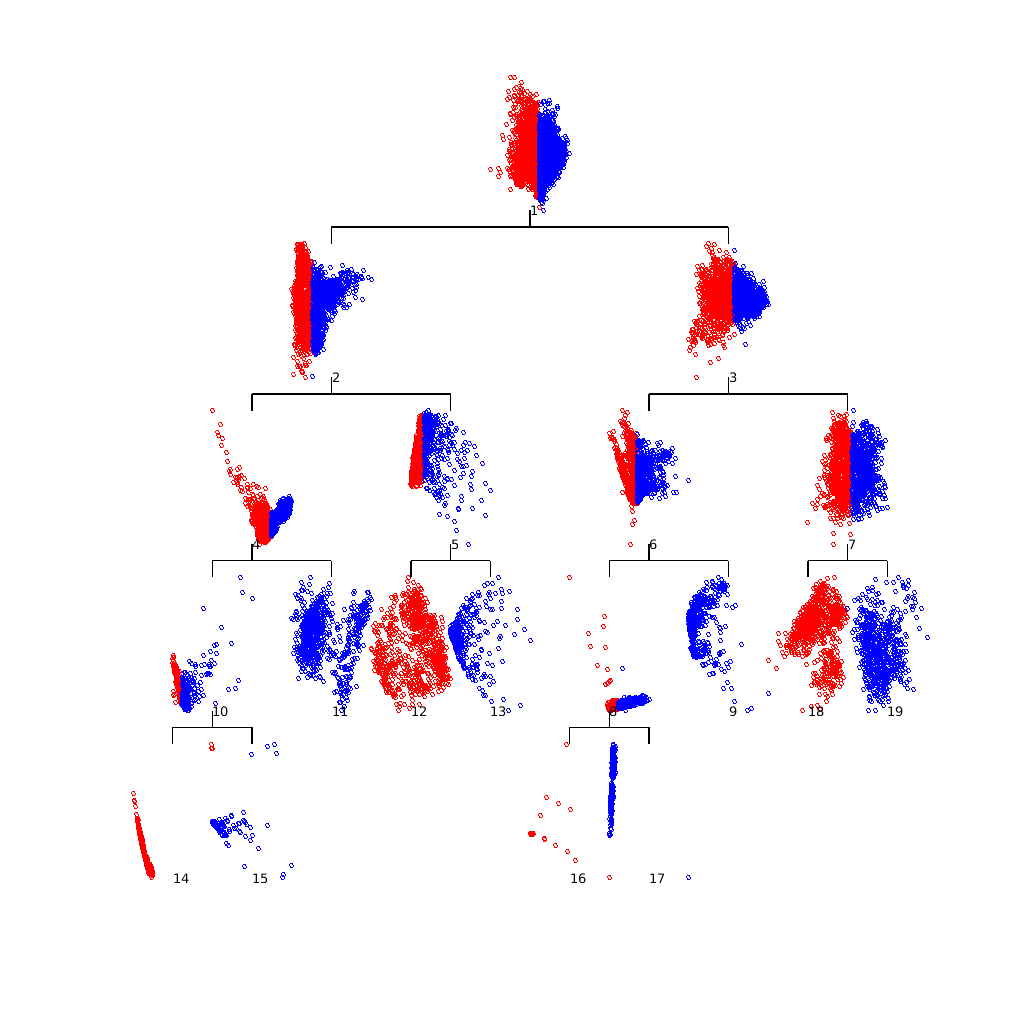
\includegraphics[scale=0.3]{figures/pddp1.png}} 
%
\subfigure[Labels specified]{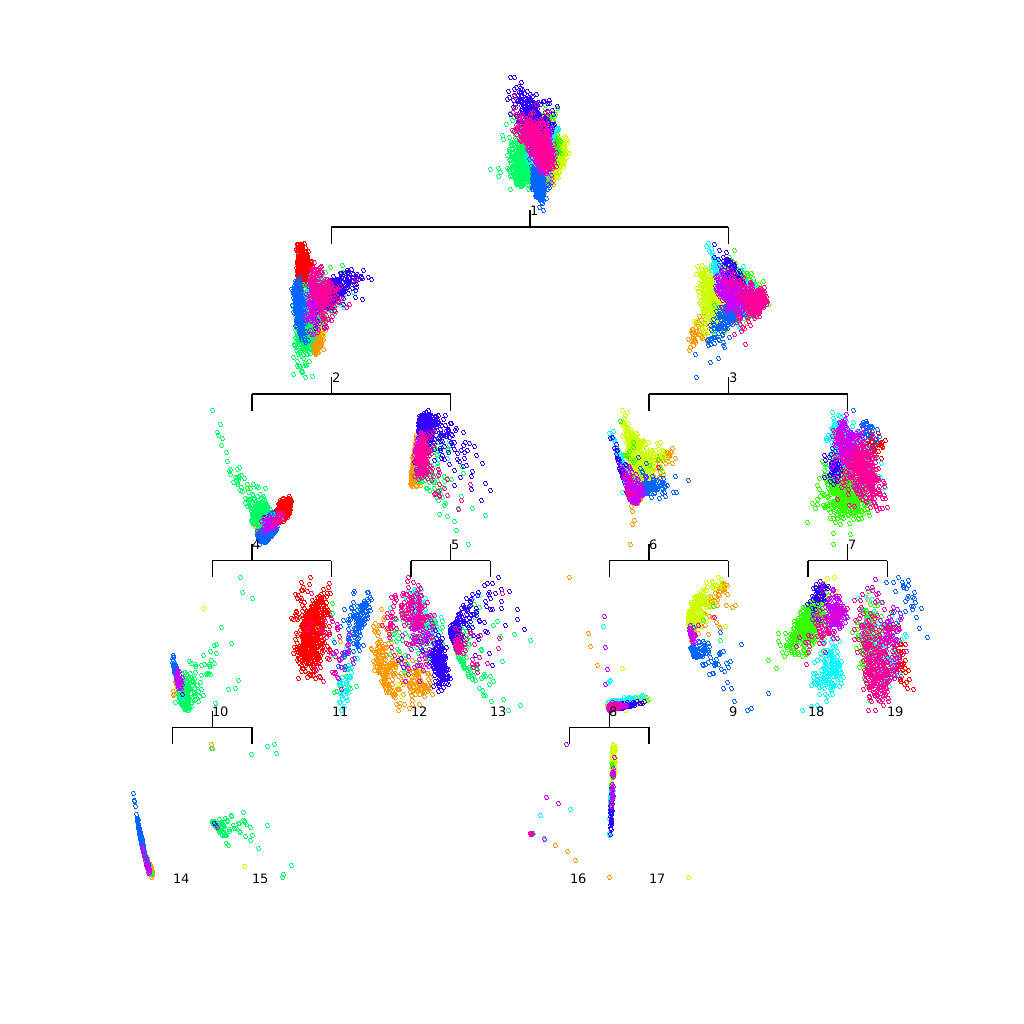
\includegraphics[scale=0.3]{figures/pddp2.png}} 
%
\end{latexonly}
	%
\begin{htmlonly}
%
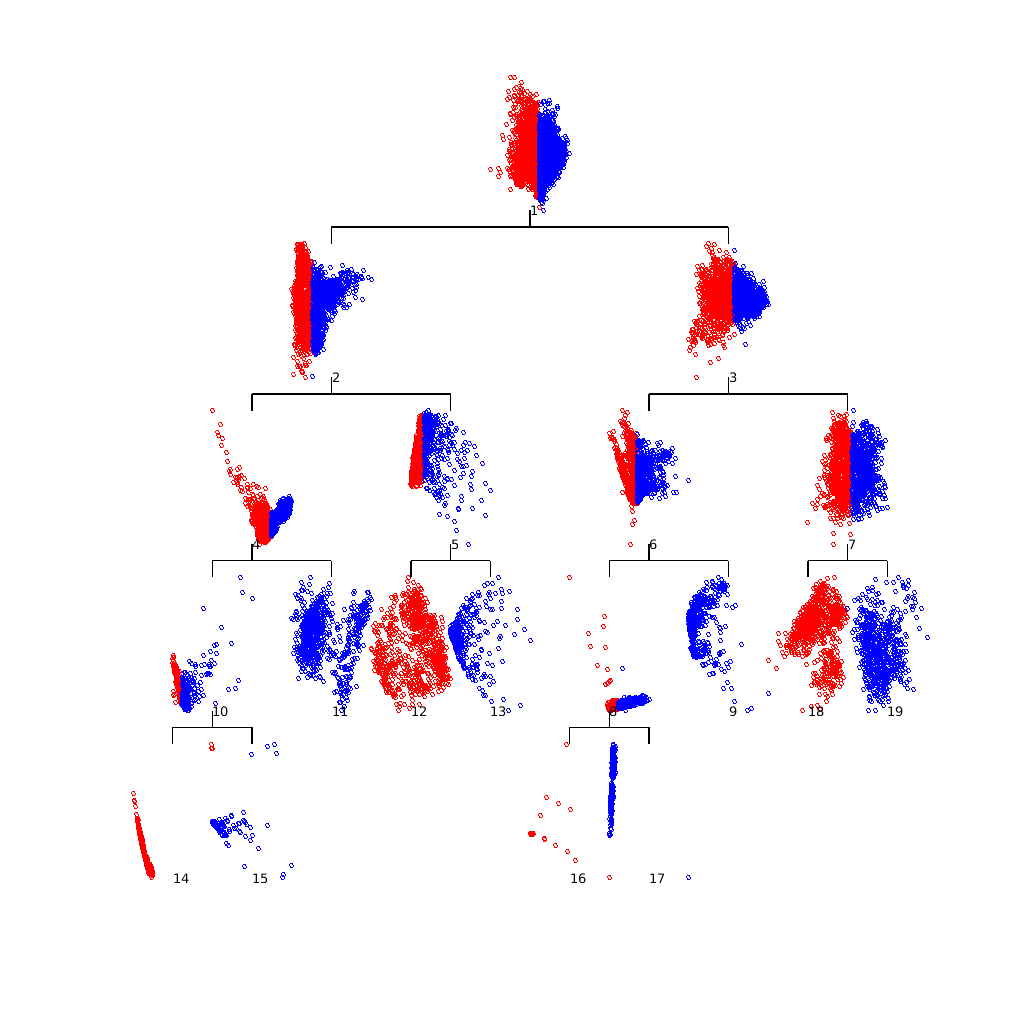
\includegraphics[scale=0.7]{figures/pddp1.png}} 
%
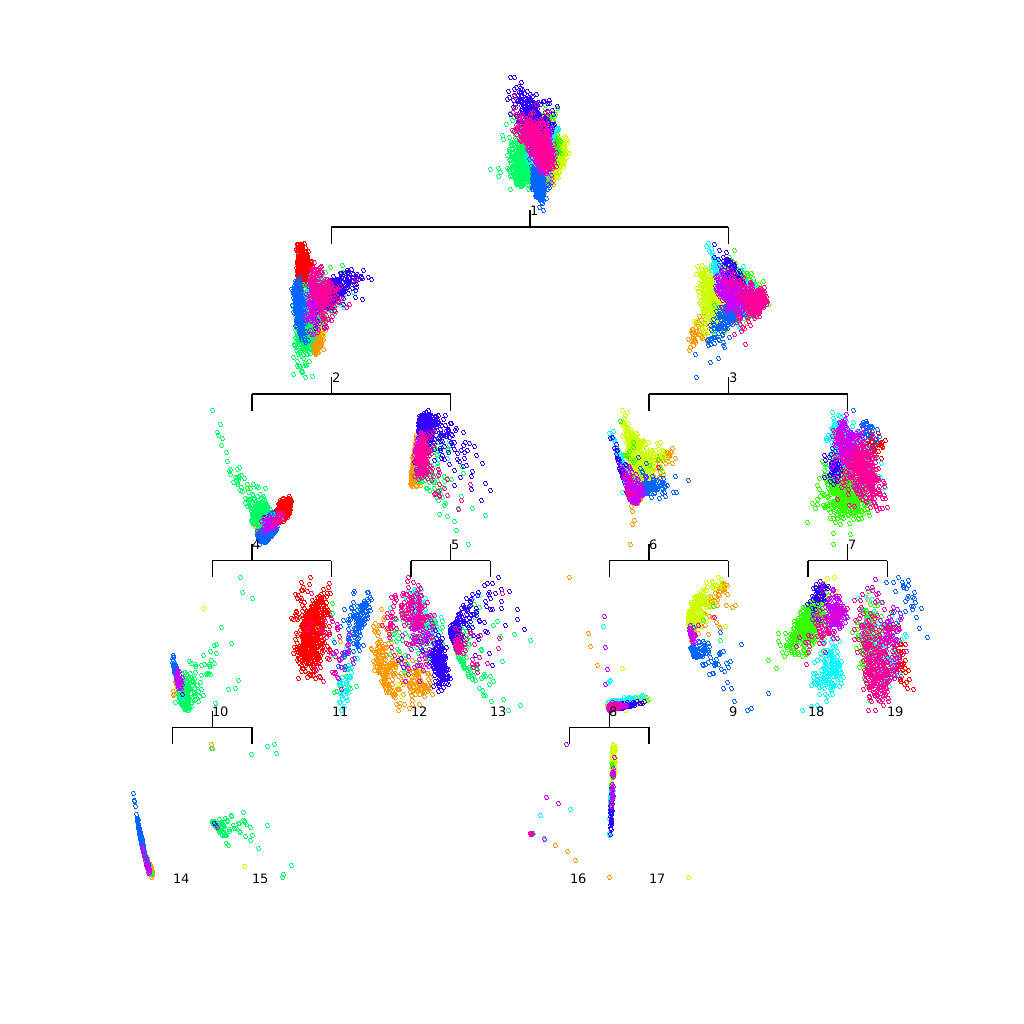
\includegraphics[scale=0.7]{figures/pddp2.png}} 
%
\end{htmlonly}
%
\caption{Visualisation of clustering model in a {\tt ctree} object without and with the
specification of the true cluster labels (left and right respectively). In the latter case
the default, {\tt hsv}, MATLAB {\tt colormap} is used.}
%
\label{fig:pddp1}
\end{figure}

\noindent
%
The output of the first two calls to the {\tt plot()} function is illustrated in
Figure~\ref{fig:pddp1}.
%
Each scatterplot in the figure depicts the data subset assigned to
the corresponding node in the hierarchy projected into a two-dimensional
subspace. In the case of algorithms that utilise one-dimensional projections
the horizontal axis corresponds to the optimal projection vector,~$v^\star$,
while the vertical axis is the direction of maximum variance orthogonal to~$v^\star$.
%
If the projection matrix contains two or more columns the {\tt plot} function
selects the two vectors along which the projected data exhibit the highest variance.
%
In the present case, because PDDP projects each data subset onto the first
principal component the vertical axis corresponds to the second principal component.

If the optional argument {\tt labels} is not specified, red and blue colours are used to
indicate the observations assigned to the left and right child of the node,
as shown in the left sub-figure in Figure~\ref{fig:pddp1}.
%
If this argument is specified then the cluster label determines
the colour of each point in the figure.
%
The user can also define the colour for each cluster, by specifying
a ({\it k} $\times$ 3) matrix, whose {\it i}--th row is the RGB triplet used to colour
the {\it i}--th cluster.

%Since leaf nodes
%correspond to clusters the projected data are assigned a single colour. When
%the \code{labels} argument is specified the points in each scatterplot are
%coloured according to their corresponding labels, as shown in
%Figure~\ref{fig:phonhierlabels}. 


Clearly the visualisation which uses the actual cluster labels to colour
observations is very informative about how the actual clusters are partitioned.
%
However, what is of more importance for unsupervised learning is that the
visualisation of the cluster hierarchy without using the actual labels also
allows the user to draw valuable insights about the validity of the binary
partitions at each node. Such insights are crucial in the process of validating
a clustering model, unless very strong assumptions about the types of
distributions that give rise to the data are imposed. This issue will be
explored further in Section~\ref{sec:valid}, but for now we provide a few
examples of insights that can be obtained from Figure~\ref{fig:pddp1}: 

\begin{itemize}

\item The splits at depth 0, 1 and 2 of the cluster hierarchy appear to be
intersecting dense regions. This could be an artefact of the visualisation
because {\tt plot} allocates the same space for the visualisation of each
binary partition, and the number of observations allocated to these nodes is
higher, compared to nodes closer to the leaves.  Therefore closer inspection is
required.

%\item The split at node 5 seems to be intersecting a dense region of the data
%and there are reasons to doubt whether this binary partition is effective.

\item The leaf nodes (clusters) 11 and 18 appear to contain at
least two dense clusters that are well separated by a sparse region. In leaf~11
the first principal component appears to be a direction which
allows the separation of the two dense clusters. For the cluster at node 18 this
does not appear to be the case.

\item The split at node 8 appears to separate a few outliers from the rest of
the data. In its right child, leaf node 17, the first principal component is
largely affected by the presence of an outlier.

\item The principal component vector (direction of maximum variance) in leaf
node number 17 is effectively determined by an outlier.

\end{itemize}


\noindent
%
The {\tt nplot} method of the {\tt ctree} class enables the visualisation of
the binary partition at any node of the cluster hierarchy. This function takes
as mandatory inputs an object of class {\tt ctree}, and the number of the node
to be visualised. It also accepts as optional arguments {\tt labels} and {\tt colours}.
The data is projected in a two-dimensional space using the same approach
as in the {\tt plot} function described previously.
%
Let's first consider the root node of the tree.

\begin{verbatim}
>> % Plot partition at root node of the cluster hierarchy
>> nplot(t1,1); 
>> % Plot partition at root node of the cluster hierarchy using actual labels
>> nplot(t1,1,labels); 
\end{verbatim}

\begin{figure}
%
\begin{latexonly}
%
\subfigure[Labels unspecified]{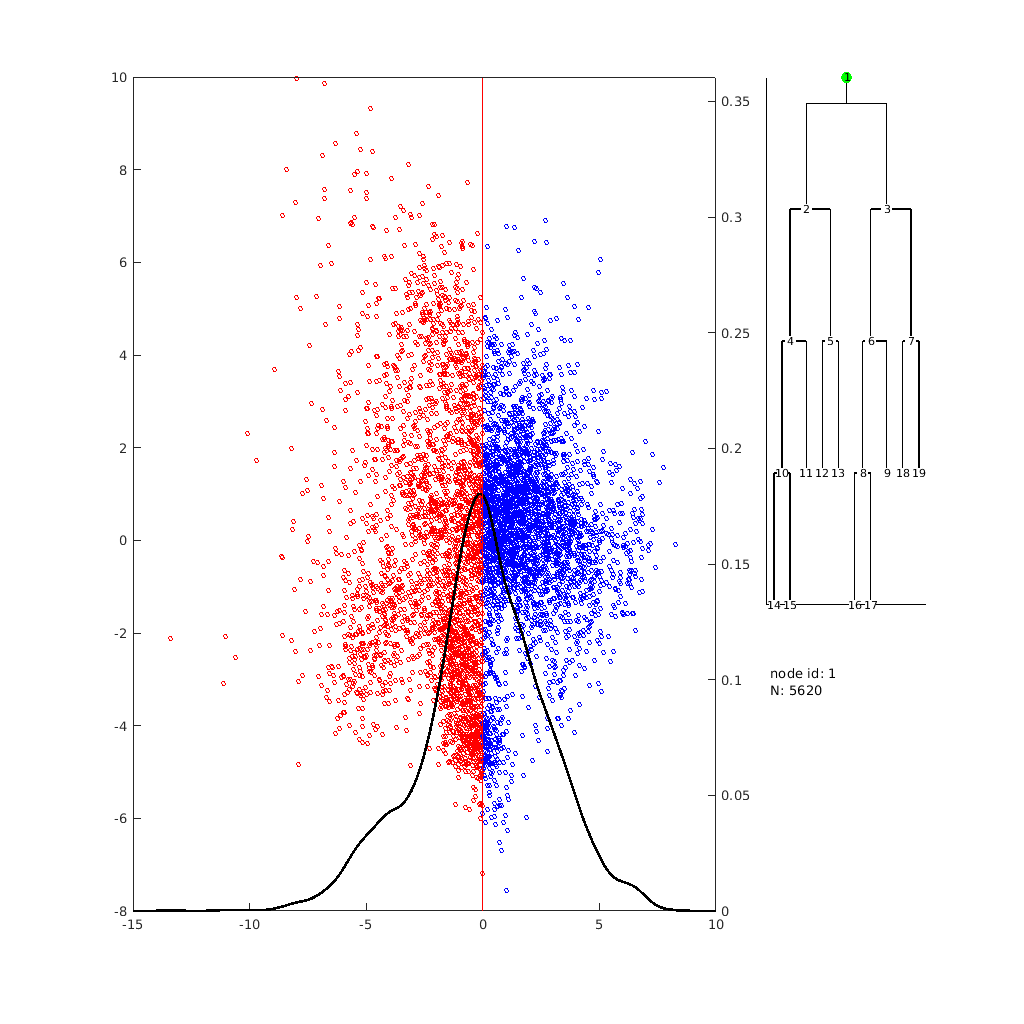
\includegraphics[scale=0.3]{figures/pddp3.png}} 
%
\subfigure[Labels specified]{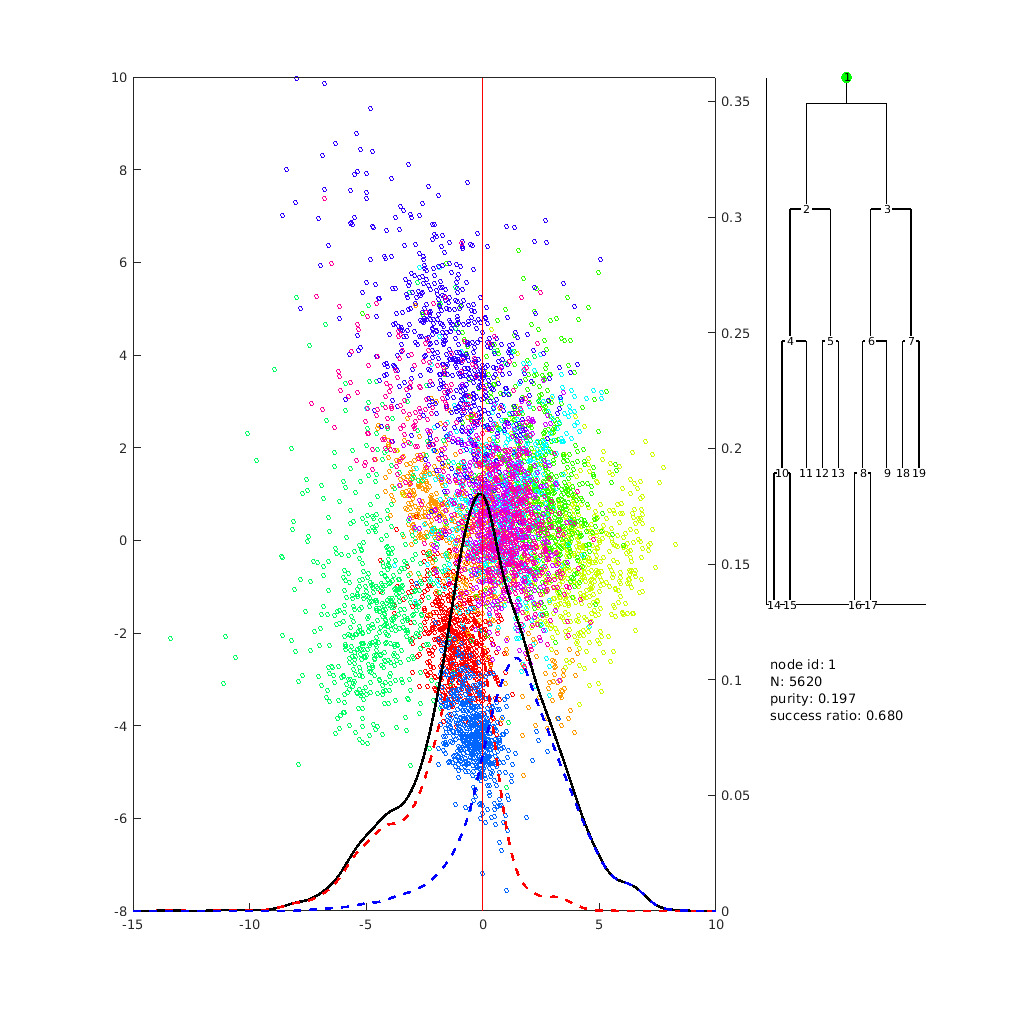
\includegraphics[scale=0.3]{figures/pddp4.png}} 
%
\end{latexonly}
%
\begin{htmlonly}
%
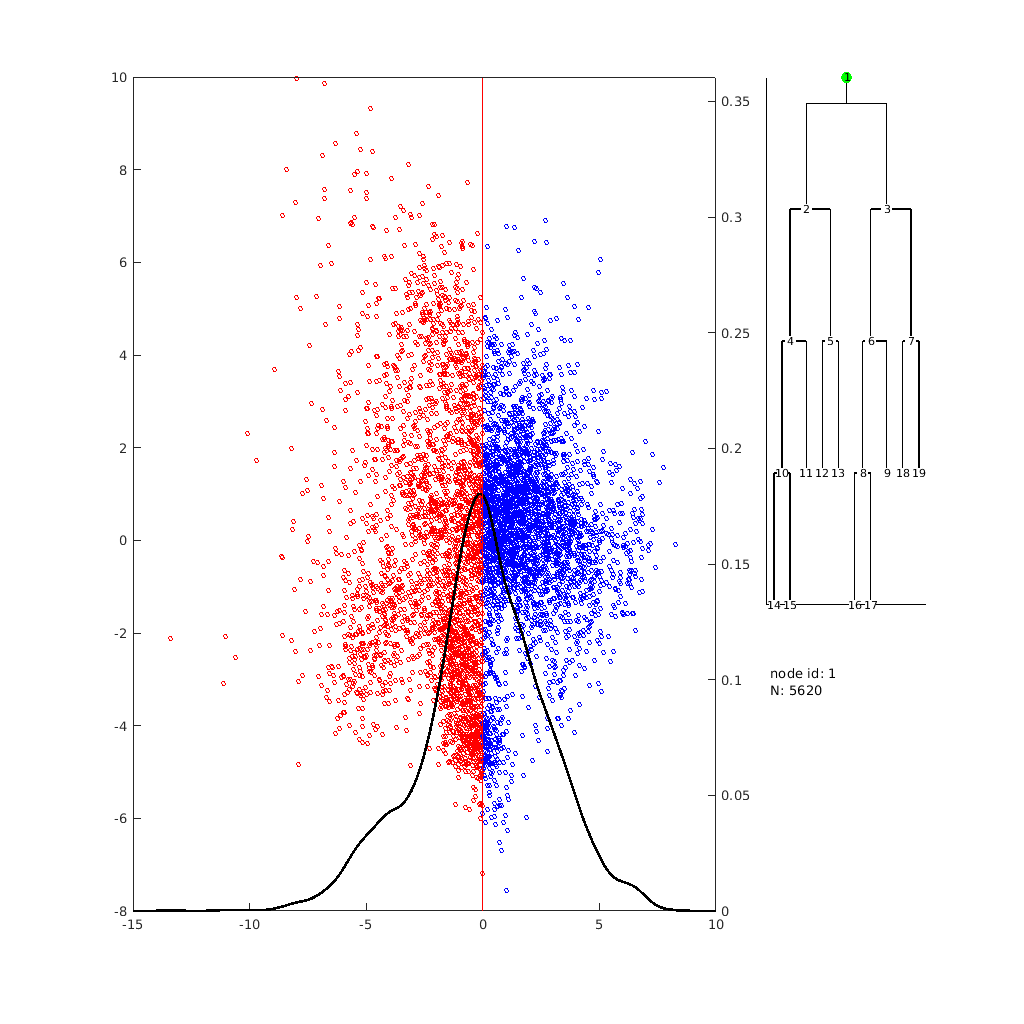
\includegraphics[scale=0.7]{figures/pddp3.png}} 
%
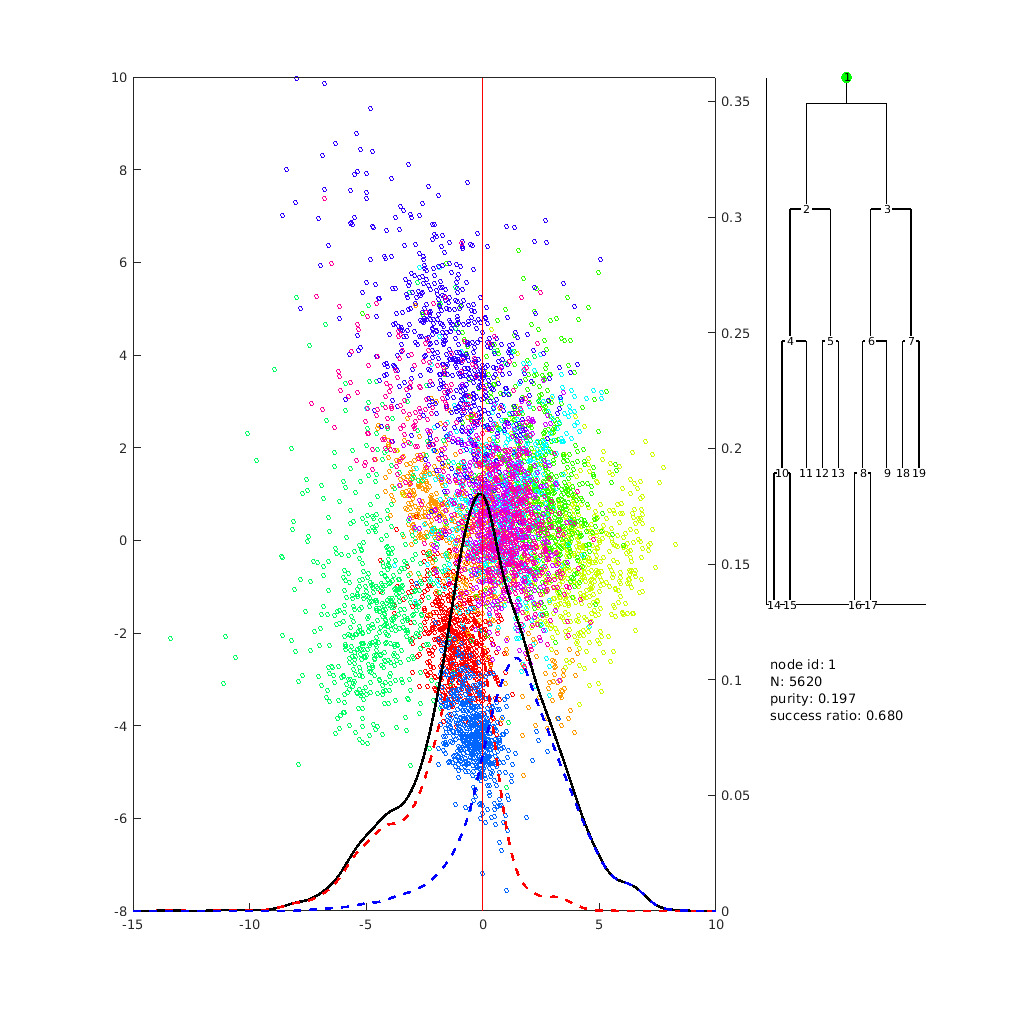
\includegraphics[scale=0.7]{figures/pddp4.png}} 
%
\end{htmlonly}
%
\caption{Visualisation of binary partition at the root node of the cluster hierarchy without and with
the specification of the true cluster labels (right and left respectively).
The black line is the kernel density estimator of the data projected onto the vector that is orthogonal
to the separating hyperplane}
%
\label{fig:pddp2}
\end{figure}

\noindent
%
Figure~\ref{fig:pddp2} (even without the labels) illustrates that the first
split of the data intersects a very dense region. The premise that underlies
PDDP, that if there are two well separated clusters in the data then these will
be separable along the first principal component, does not appear to be valid
in this example.


When the clustering algorithm uses a hyperplane to bi-partition the data at
each node, the {\tt nplot} function also illustrates a kernel density estimator
constructed from the projection of the data onto the vector orthogonal to the
separating hyperplane (black line). The scale of this function is illustrated
on the right vertical axis.
%
If the true clusters labels are specified, as in the second sub-figure in
Figure~\ref{fig:pddp2}, then each cluster is assigned to the halfspace that
contains the majority of its observations. The overall density can then be seen
as a two component mixture arising from the clusters assigned to the
two halfspaces. The red and blue solid lines illustrate these two component
densities. This visualisation is intended to highlight the extend to which the
separating hyperplane splits clusters in the data.
%
The fact that in Figure~\ref{fig:pddp2} the two densities overlap considerably is a
clear indicator that this hyperplane is splitting clusters.


\subsection{Quality of a Binary Partition}

The {\em success ratio} is a measure of how
effectively a binary partition separates at least one cluster from the
rest, in datasets that contain two or more clusters~\cite{PavlidisHT2016}. This measure
is always between zero and one, with higher values indicating better performance.
%
To estimate the success ratio for a specific
binary partition we will use the information from the {\tt ctree}
object that stores the cluster hierarchy.
%
To access a node of this object we can use the method {\tt get} of the {\tt
ctree} class. Each node of the tree is a structured array. The {\tt idx}
element of this array contains the indices (row numbers in the data matrix {\tt
X}) of the observations allocated to this node. Observations allocated to the
left child of a node have negative sign while those allocated to the right
child have a positive sign. The code snippet below uses these properties to
estimate the success ratio at the root of the {\tt tt} object.

\begin{verbatim}
>> % Get root node of cluster hierarchy
>> node1 = t1.get(1);
>> % Assess quality of binary partition through success ratio
>> success_ratio(sign(node1.idx), labels)
\end{verbatim}


It is possible to evaluate the success ratio at each node of the cluster hierarchy,
using the method {\tt perf} of the {\tt ctree} class. 

\begin{verbatim}
>> % Evaluate performance at each node of t1
>> t1 = perf(t1, labels)
\end{verbatim}

\noindent
The output of the above function is displayed on the terminal. It is unfortunately
too large to be included here.

\subsection{density-enhanced PDDP}

We next consider whether the splitting criterion used by dePDDP will
improve the clustering result.


\begin{verbatim}
>> [idx2, t2] = depddp(X,10);
Clusters: 1 2 3 4 Divisive process terminated because no cluster can be split further
Clusters Identified: 4
\end{verbatim}

\noindent
%
The output above indicates that this algorithm did not manage to estimate the
10 clusters that we requested. The dePDDP algorithm fails to partition a
cluster when the one-dimensional kernel density estimator constructed from the
projection of the data onto the first principal component is unimodal.
This is considered an indication that the data belong to a single cluster.

\begin{figure}
%
\begin{latexonly}
%
\subfigure[Cluster hierarchy]{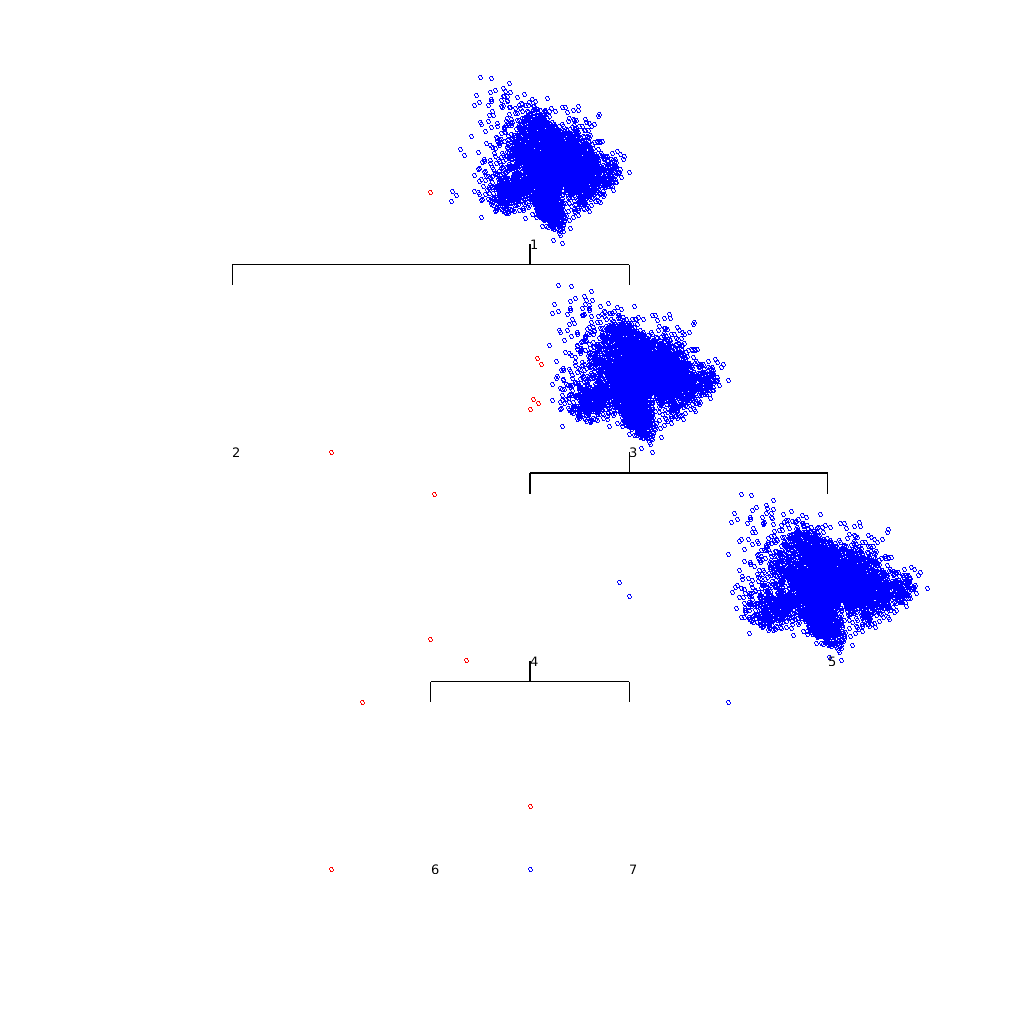
\includegraphics[scale=0.3]{figures/depddp1.png}} 
%
\subfigure[First binary partition]{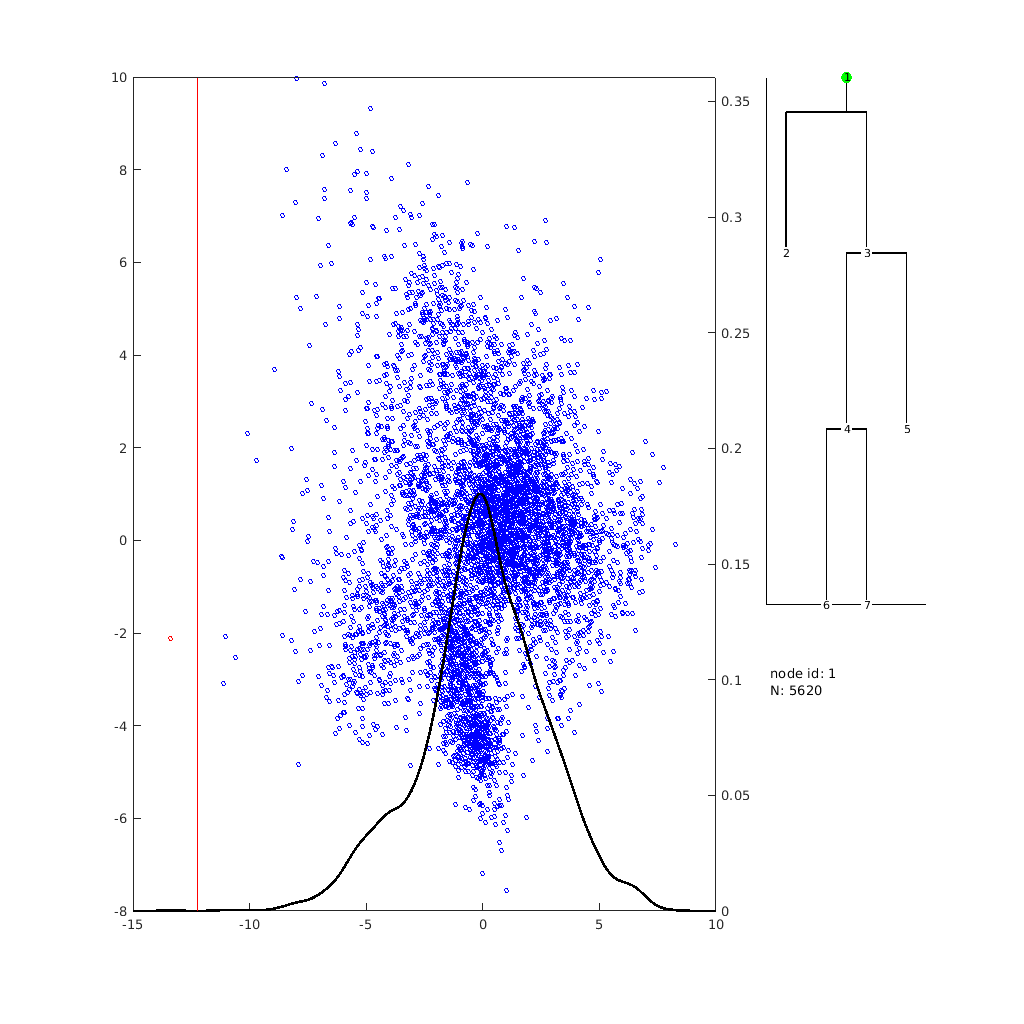
\includegraphics[scale=0.3]{figures/depddp2.png}} 
%
\end{latexonly}
%
\begin{htmlonly}
%
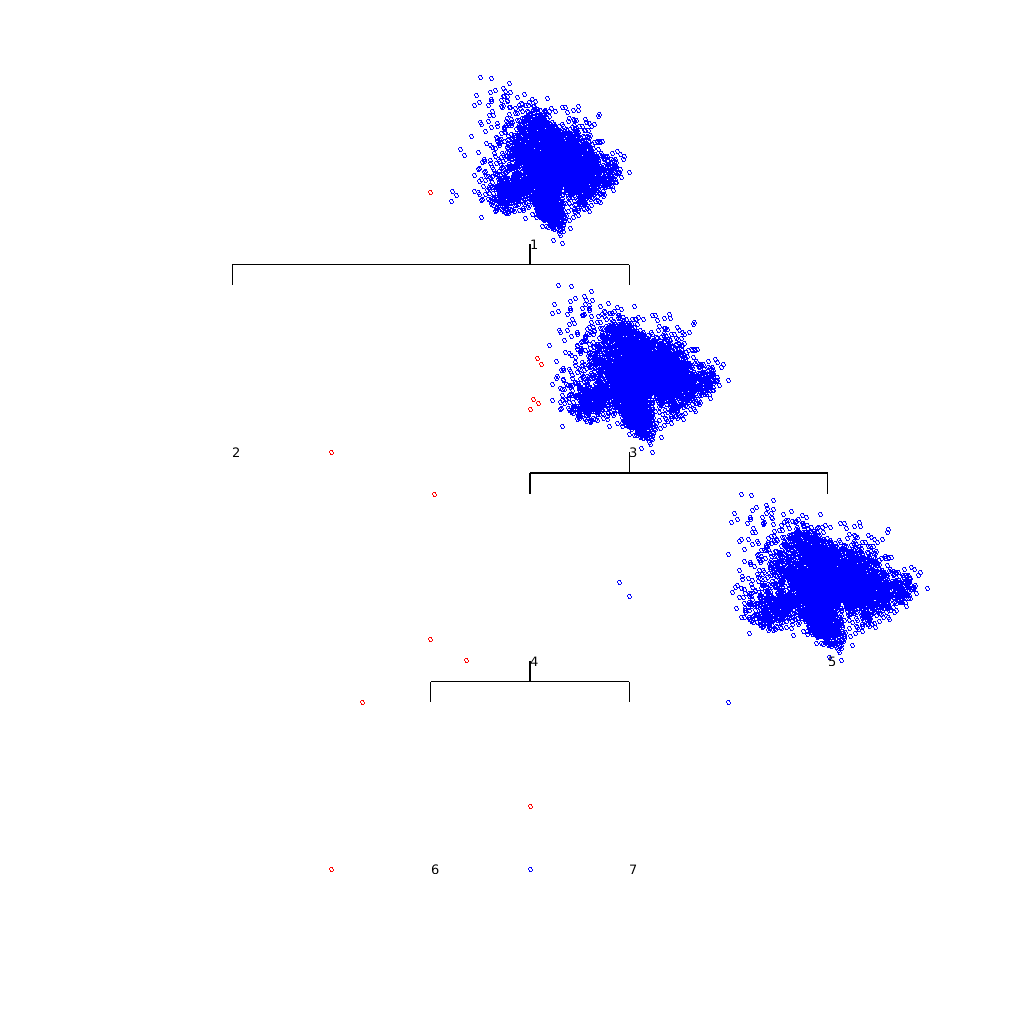
\includegraphics[scale=0.7]{figures/depddp1.png}} 
%
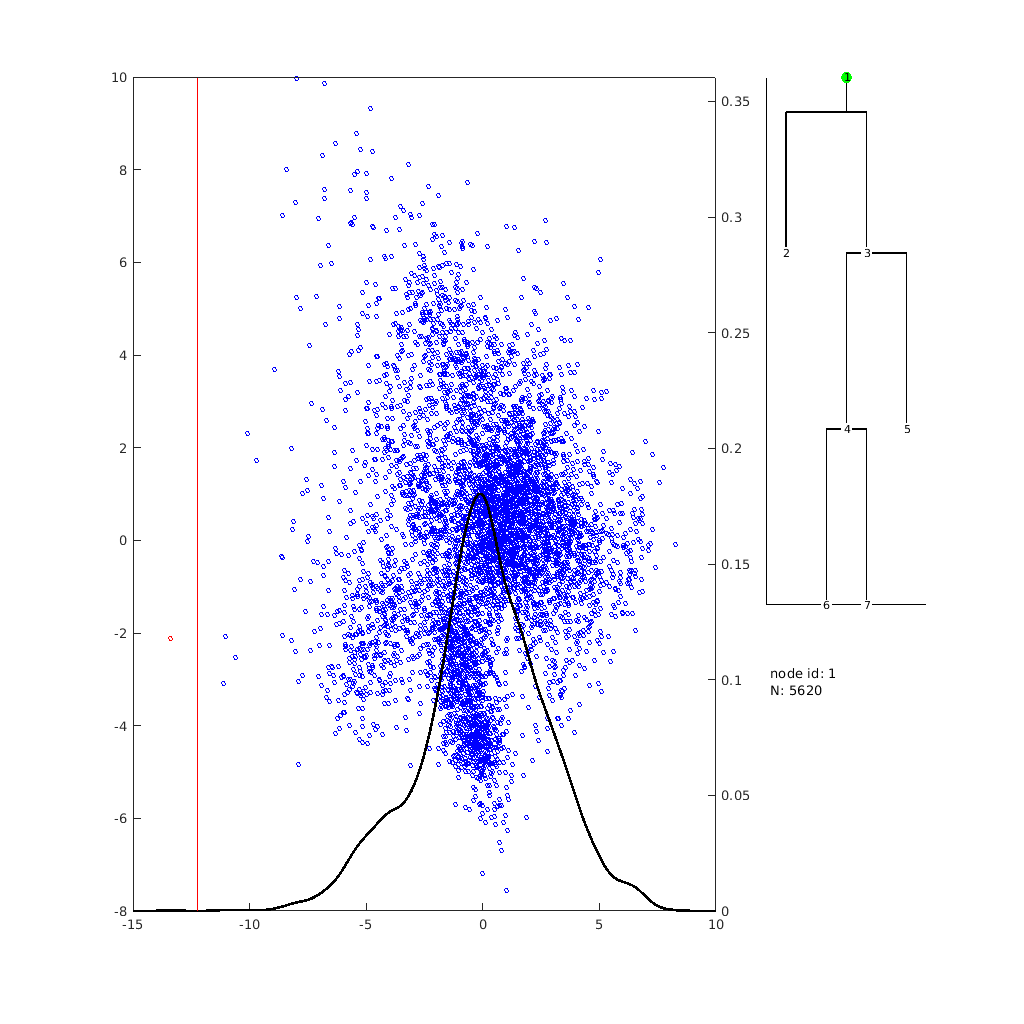
\includegraphics[scale=0.7]{figures/depddp2.png}} 
%
\end{htmlonly}
%
\caption{Visualisation of cluster hierarchy and first binary partition performed by
dePDDP}
%
\label{fig:depddp1}
\end{figure}


Figure~\ref{fig:depddp1} illustrates the clustering model created by this
algorithm, as well as the binary partition at the root node. From this figure
we see why the algorithm failed to estimate 10~clusters and why the clustering
model produced is not valid for this dataset.
%
The one-dimensional projection of the data onto the first principal component 
always contains one or a few
observations that are very distant from the rest. The estimated density
has a very small mode at these observations and as a result at each
bi-partition dePDDP splits one or a few outliers from the rest of the
data. Around the bulk of the data the density estimator is unimodal.

A naive approach to overcome this limitation would be to impose
a constraint on the minimum number of points in a cluster. This option
is available in all divisive hierarchical clustering algorithms in OPC.

\begin{verbatim}
>> [idx2, t2] = depddp(X,10,'minsize',10);
Clusters: 1 Divisive process terminated because no cluster can be split further
Clusters Identified: 1
\end{verbatim}

\noindent
%
The above message indicates that with a minimum cluster size of 10 the
data cannot be split.
%
This should not be surprising as we can see from Figure~\ref{fig:depddp1}
that the density estimator has no local minima apart from the one at its left tail.
%

An important parameter in dePDDP is the bandwidth used in the density
estimator. By default dePDDP estimates the bandwidth
parameter, $h$, through the rule suggested by Silverman~\cite{Silverman1986}
for the approximation of multimodal univariate densities,
%
\[
h = 0.9 n^{-1/5} \hat{\sigma}, 
\]
%
where $\hat{\sigma}$ is the standard deviation of the projected data.
%
The user can modify this by providing as input a function handle.
The associated function must take as input a data matrix and a structured array
containing the algorithm's parameters, and return a positive scalar. This function
is used to estimate the value of the bandwidth parameter for each cluster.
In the next code snippet we halve the value of the bandwidth.

\begin{verbatim}
>> % Define function handle to set bandwidth
>> fh = @(x,p)(0.45*size(x,1)^(-0.2)*std(x* pcacomp(x,1)));
>> [idx2, t2] = depddp(X,10,'minsize',100, 'bandwidth', fh);
Clusters: 1 2 3 4 5 6 7 8 9 10
\end{verbatim}
%

\noindent
%
%The {\tt pcacomp} function used in the definition of the function handle
%returns the principal component(s) specified in its second argument (in the
%order they are specified).
%%
dePDDP with these settings can estimate
10 clusters, but a visualisation of the clustering model produced (which is
omitted for brevity) illustrates that this model does not overcome any of
the previously identified problems.


The inspection of the clustering models produced by PDDP and dePDDP strongly
suggests that for this dataset dimensionality reduction by projecting onto the
first principal component is not appropriate.
%
In the next section we explore algorithms that attempt to identify the optimal
projection vector with respect to explicit clustering criteria.
%

\section{Divisive Clustering based on Optimal Hyperplanes}

First we consider divisive clustering algorithms obtained by recursively
bi-partitioning the data through hyperplanes that are estimated by identifying
the optimal one-dimensional data projection. Three such methods will be
discussed.  The Maximum Clusterability Divisive Clustering (MCDC) algorithm
attempts to identify the one-dimensional projection that optimises variance
ratio clusterability; a criterion connected to the {\it k}--means objective
function. The second method recursively bi-partitions the data using the
minimum Normalised Cut Hyperplane (NCUTH) algorithm, which attempts to identify
the projection vector that minimises the value of the normalised graph-cut
criterion. The last method, Minimum Density Divisive Clustering (MCDC) attempts
to identify the hyperplane along which the integral of the estimated density is
minimised.


For methods based on separating hyperplanes, OPC also includes a separate
implementation of the underlying binary segmentation algorithm. To distinguish between the two,
the names of functions that produce a complete divisive clustering model end in {\tt dc},
while those that perform a single binary partition using a hyperplane as a
cluster separator, end in {\tt h}.
%
For example, the MCDC algorithm is implemented in the {\tt mcdc} function,
while the {\tt mch} function estimates a single maximum clusterability
hyperplane.

\subsubsection{Maximum Clusterability Divisive Clustering}

The MCDC algorithm is implemented in the function {\tt mcdc}.

\begin{verbatim}
>> [idx3,t3] = mcdc(X,10);
>> cluster_performance(idx3,labels)

ans = 

  struct with fields:

      Purity: 0.7710
         NMI: 0.7174
     AdjRand: 0.6371
    Vmeasure: 0.7174

>> plot(t3);
>> nplot(t3,1);
\end{verbatim}

\noindent
%
The clustering performance of this algorithm improves that of {\it k}--means applied
on the full dimensional data, as well as that of {\it k}--means applied on
the data projected onto the first 9 or 33~principal components.

It is important to note
that the initialisation of the projection pursuit algorithm in MCDC is performed by
applying 2-means on the data (subset) and computing the vector that connects
the cluster centroids. Since by default {\tt kmeans} in MATLAB
and Octave uses the {\it k}--means++ algorithm~\cite{ArthurV2007}, 
the output {\tt mcdc} can differ in consecutive executions with
identical input parameters.


\begin{figure}
%
\begin{latexonly}
%
\subfigure[Cluster hierarchy]{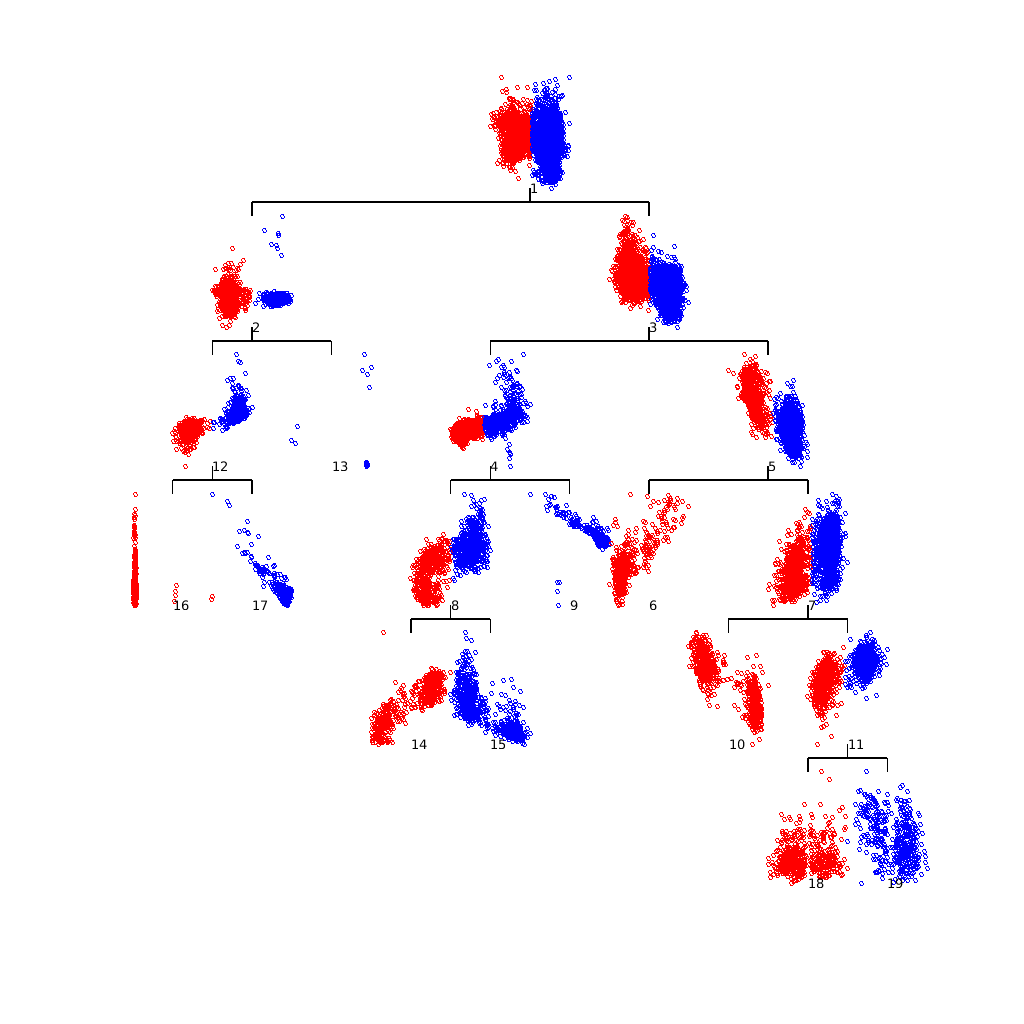
\includegraphics[scale=0.3]{figures/mcdc1.png}} 
%
\subfigure[First binary partition]{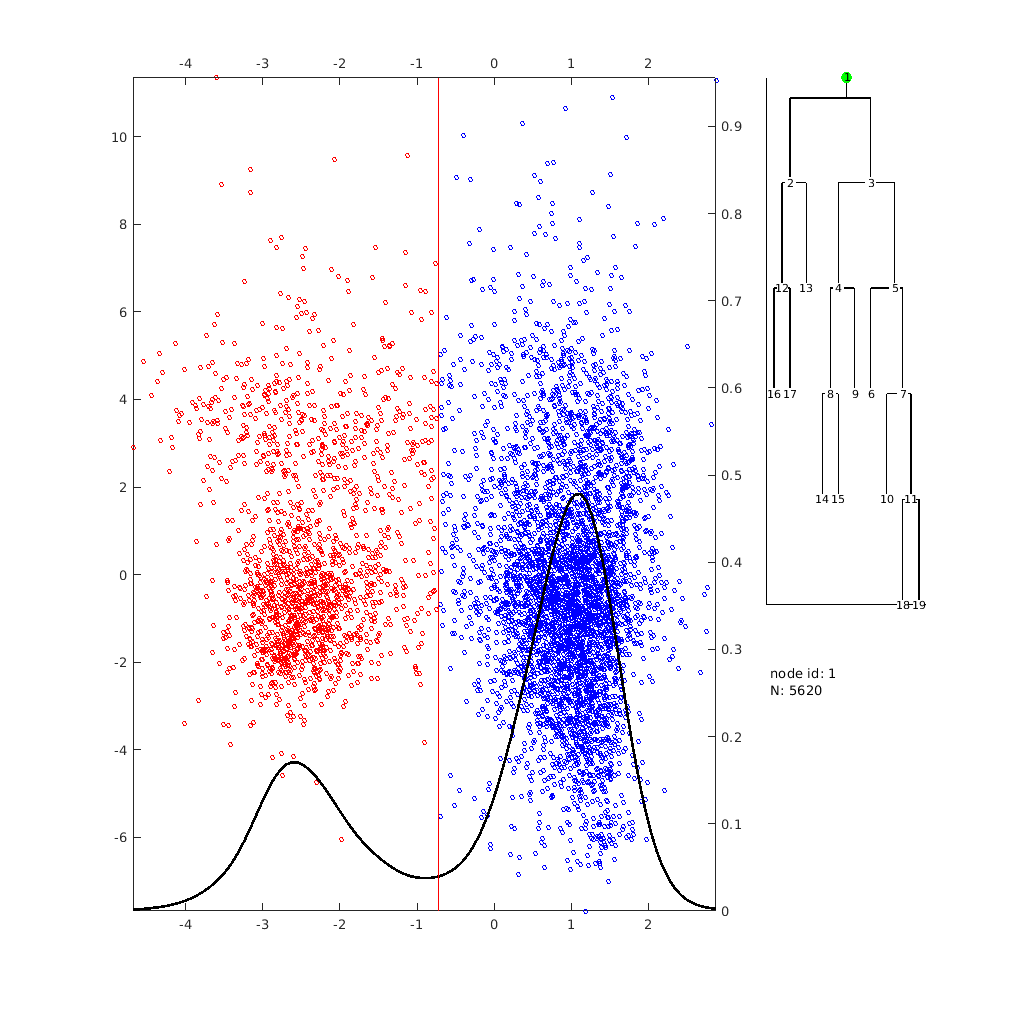
\includegraphics[scale=0.3]{figures/mcdc2.png}} 
%
\end{latexonly}
%
\begin{htmlonly}
%
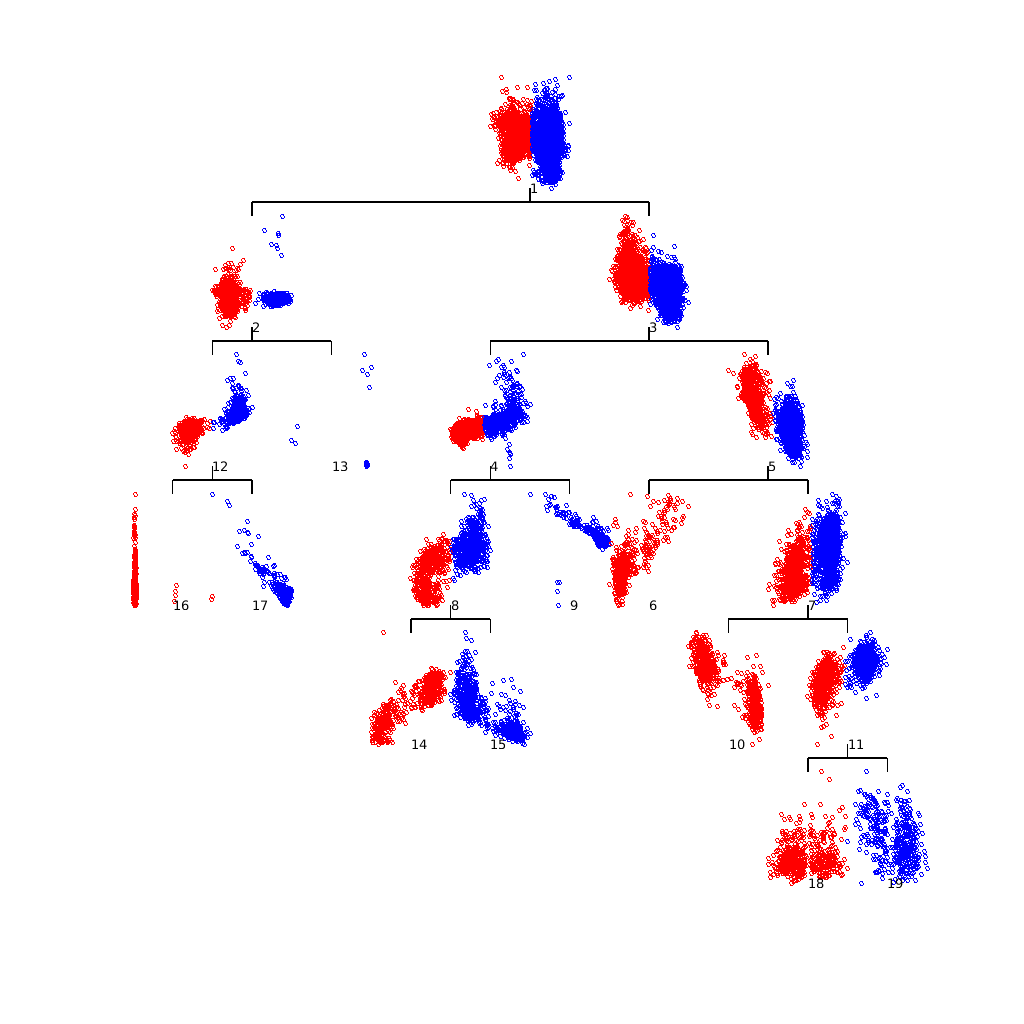
\includegraphics[scale=0.7]{figures/mcdc1.png}} 
%
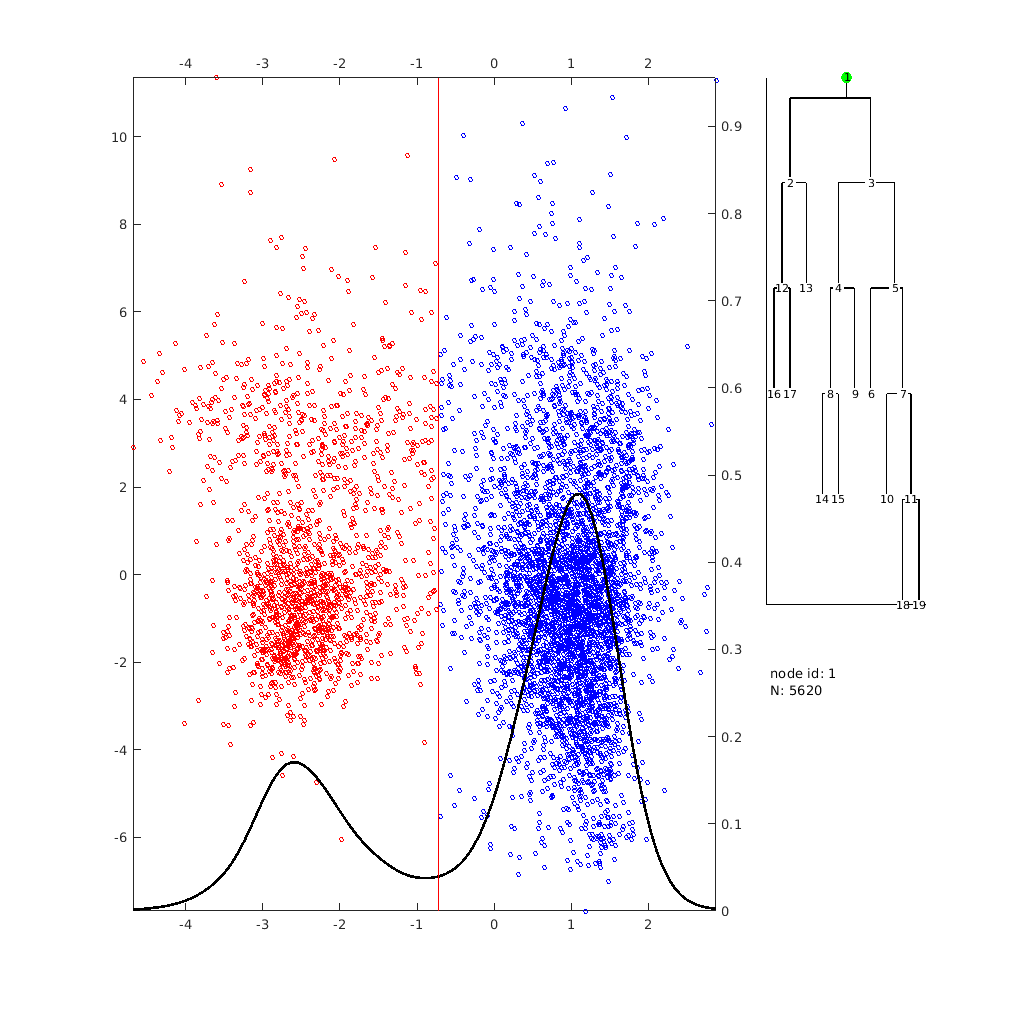
\includegraphics[scale=0.7]{figures/mcdc2.png}} 
%
\end{htmlonly}
%
\caption{Visualisation of cluster hierarchy and first binary partition performed by MCDC}
%
\label{fig:mcdc1}
\end{figure}


The plot of the model hierarchy, and the first binary partition is provided in
Figure~\ref{fig:mcdc1}.
%
The figure shows that MCDC performs a much more sensible clustering, compared
to PDDP and dePDDP. The visualisation of the binary partition at the root of
the tree clearly shows that the projection pursuit algorithm has managed to
identify a hyperplane that traverses a relative sparse region and separates two
dense clusters. This provides clear evidence of a clustering structure in the
data which was not visible through PDDP and dePDDP (Figures~\ref{fig:pddp2}
and~\ref{fig:depddp1}, respectively).
%
Inspecting the visualisation for the entire clustering model one observes that
the majority of binary partitions at internal nodes appear to be separating
effectively dense clusters. 
%
%The split at node~9 appears to be separating out a few outliers from the bulk
%of the data, but subsequent splits appear reasonable. 
%
A number of leaves appear to contain more than one cluster and are natural
candidates for further splitting. 
%
An extensive example of using OPC to validate and modify a clustering model is
provided in Section~\ref{sec:valid}.



We can examine whether an alternative initialisation would improve the final
clustering model. In the example below we set the initial projection vector to
be the first principal component. This is achieved by specifying the optional argument
{\tt v0}. For divisive hierarchical clustering algorithms this input argument
must be set to a function handle.
The associated function must accept two inputs:
the data matrix, and a structured array containing the parameters of the algorithm.
%
Note that by using the first principal component to initialise the projection
pursuit algorithm at each bi-partition {\tt mcdc} becomes deterministic. 

\begin{verbatim}
>> % Function handle returns 1st PC
>> fh = @(x,p)(pcacomp(x,1));
>> [idx4,t4] = mcdc(X,10,'v0', fh);
>> 
>> % Assess clustering performance
>> cluster_performance(idx4,labels);

ans = 

  struct with fields:

      Purity: 0.7466
         NMI: 0.6727
     AdjRand: 0.5760
    Vmeasure: 0.6727

\end{verbatim}

\noindent
%
This initialisation causes a small deterioration in clustering performance. The visualisation
of the resulting clustering model in Figure~\ref{fig:mcdc2} reveals that the
resulting clusters are more balanced, but there still remain clear indications that some leaves of the
hierarchy contain more than one cluster, and should therefore be split.
%
\begin{figure}
%
\begin{latexonly}
%
%\subfigure[Cluster hierarchy]{
\begin{center}
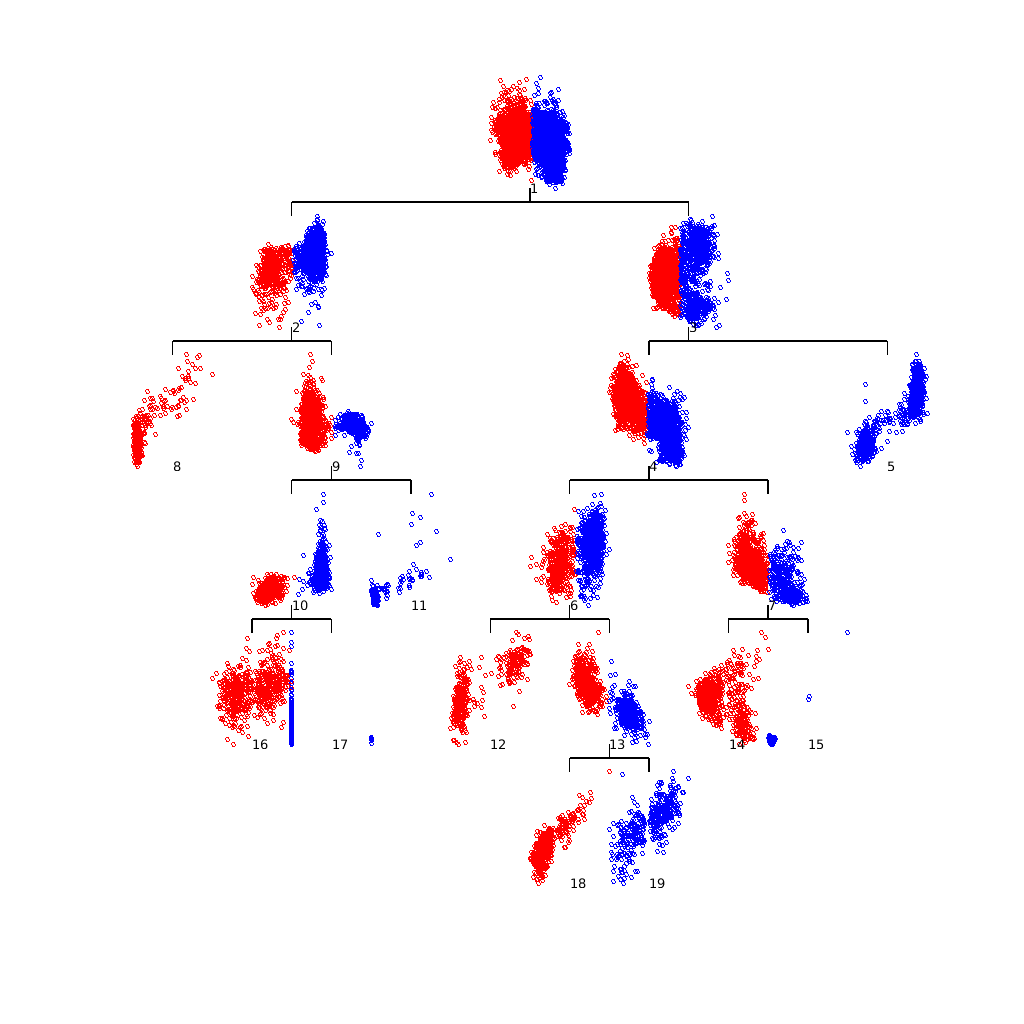
\includegraphics[scale=0.3]{figures/mcdc3.png}
\end{center}
%}
%
%\subfigure[First binary partition]{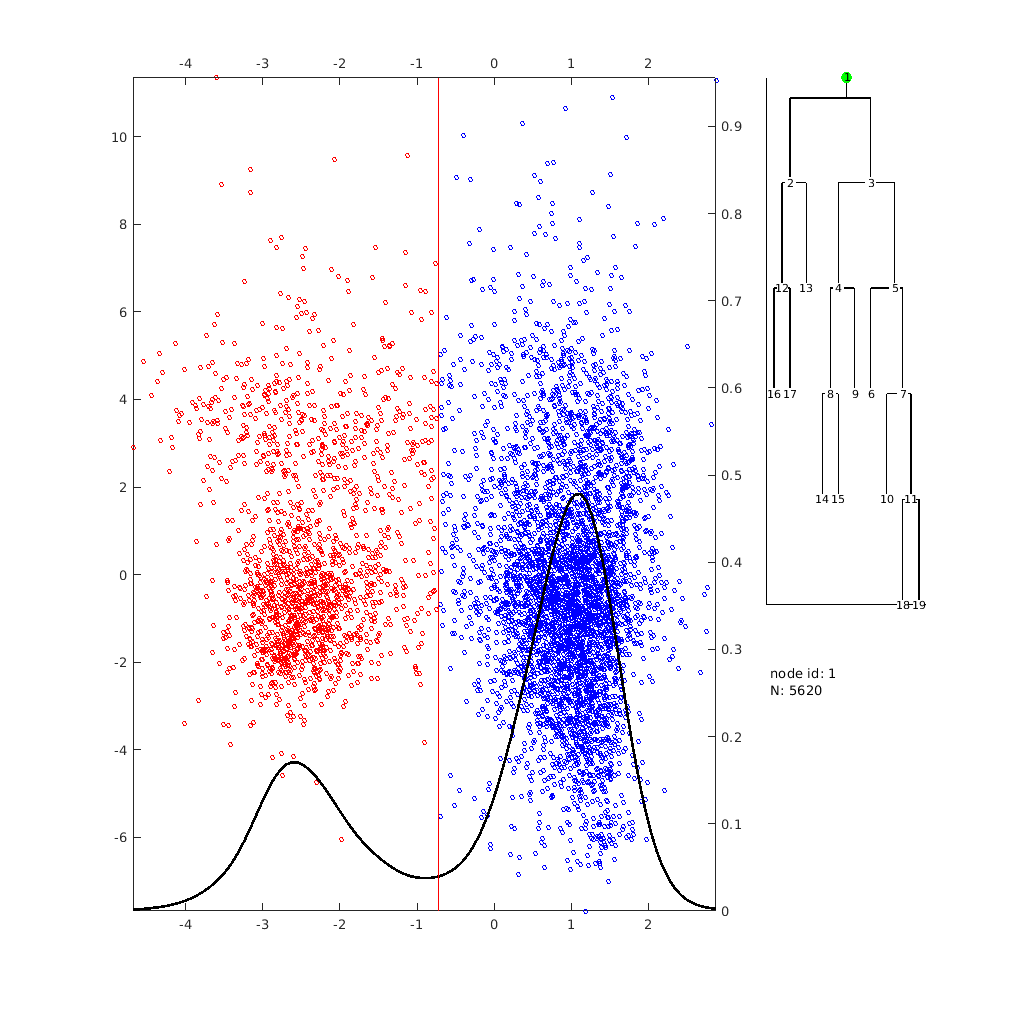
\includegraphics[scale=0.3]{figures/mcdc2.png}} 
%
\end{latexonly}
%
\begin{htmlonly}
%
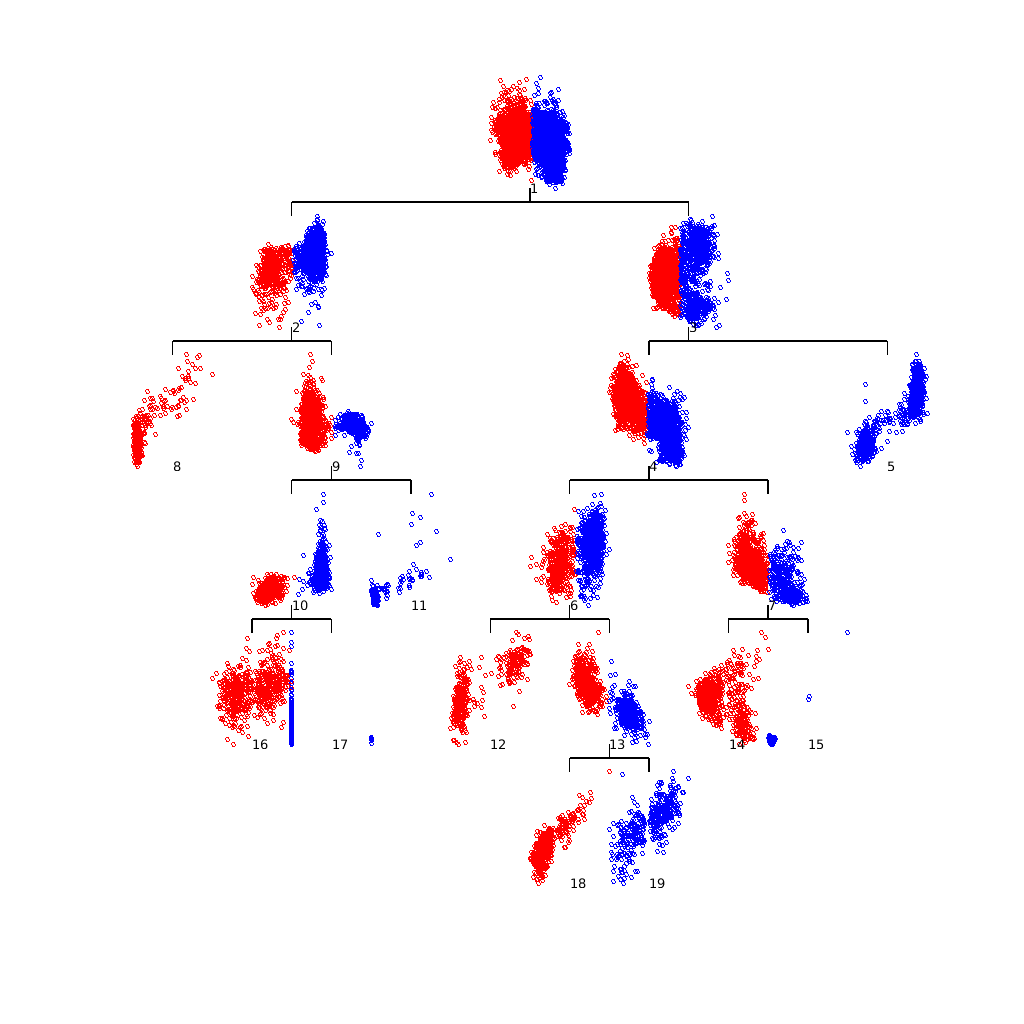
\includegraphics[scale=0.7]{figures/mcdc3.png}
%
%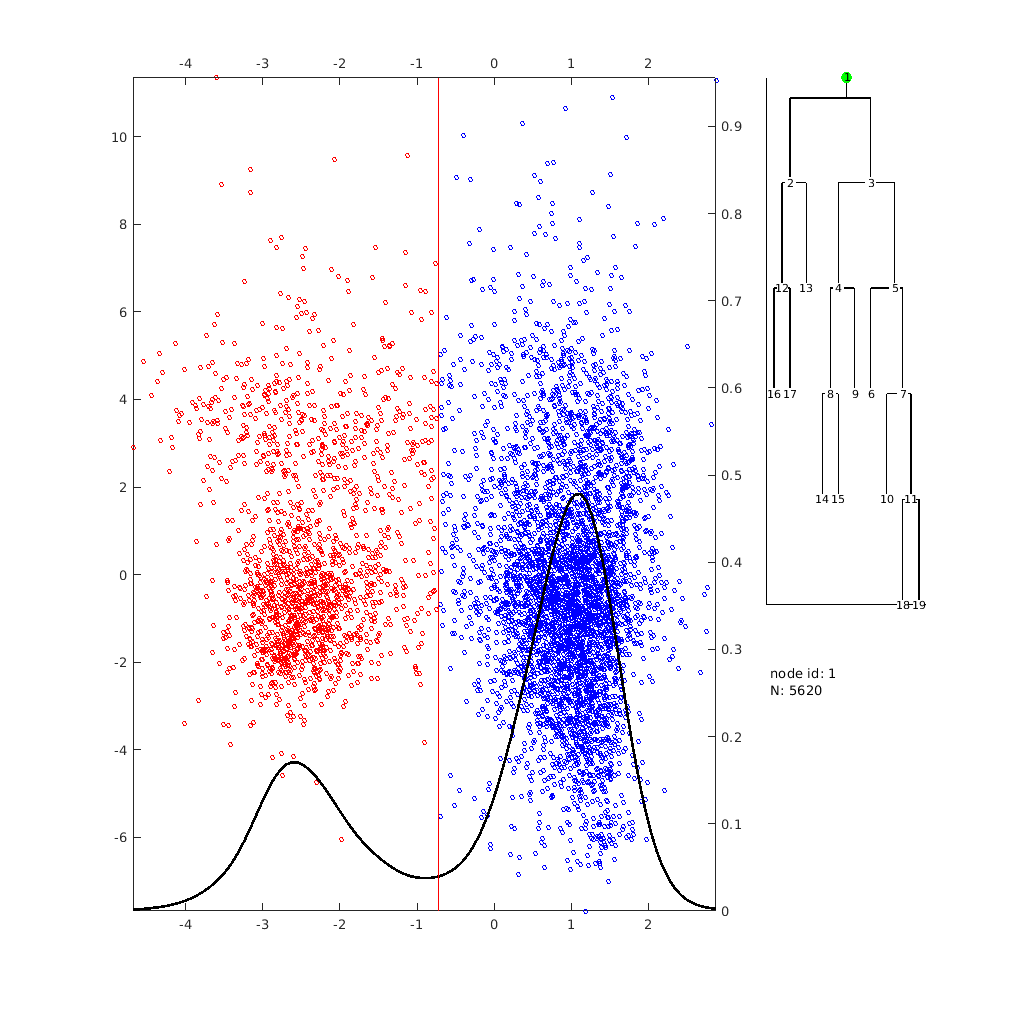
\includegraphics[scale=0.7]{figures/mcdc2.png}} 
%
\end{htmlonly}
%
\caption{MCDC cluster hierarchy using first principal component to initialise
projection pursuit algorithm}
%
\label{fig:mcdc2}
\end{figure}

%Lastly we provide an example of how to modify the choice of the cluster which will be
%split at each step of a divisive algorithm. This is achieved by specifying the
%optional argument {\tt split\_index}. This argument must be set to a handle to a function
%that returns a scalar and takes three inputs: the projection matrix (vector in this case),
%the data matrix and a structured array containing parameters of the algorithm.
%%
%At each step of any divisive clustering algorithm, the cluster with the maximum
%value of the split index is partitioned. In the next example we set the split index
%to be equal to the size of the cluster, causing {\tt mcdc} to split the largest cluster at each step.
%%
%\begin{verbatim}
%>> [idx4,t4] = mcdc(X,10,'split_index', @(v,x,p)(size(x,1));
%\end{verbatim}


\subsection{Minimum Normalised Cut Divisive Clustering}

We next produce a clustering model using the minimum Normalised Cut Divisive Clustering
(NCUTDC) algorithm. 

\begin{verbatim}
>> [idx5,t5] = ncutdc(X,10);
>> 
>> % Assess clustering performance
>> cluster_performance(idx5,labels);

ans = 

  struct with fields:

      Purity: 0.7810
         NMI: 0.6950
     AdjRand: 0.6200
    Vmeasure: 0.6949

\end{verbatim}

\noindent
%
NCUTDC performs better than spectral clustering applied on the
full--dimensional data, and the datasets obtained after projection onto the
first 9 and 33 principal components.  This indicates that the dimensionality
reduction approach is enabling the algorithm to identify better quality
clusters. The resulting cluster hierarchy is illustrated in Figure~\ref{fig:ncut1}.

%However, a closer visualisation of the binary partition at individual nodes
%of the hierarchy reveals evidence that the hyperplane separator at node~3
%(illustrated in Figure~\ref{fig:ncut1}) does not appear to separate well
%distinguished clusters.
%A poor split early
%in the cluster hierarchy is problematic because it affects the entire subtree
%rooted at this node.
%
\begin{figure}
%
\begin{latexonly}
%
\begin{center}
%\subfigure[Cluster hierarchy]{
	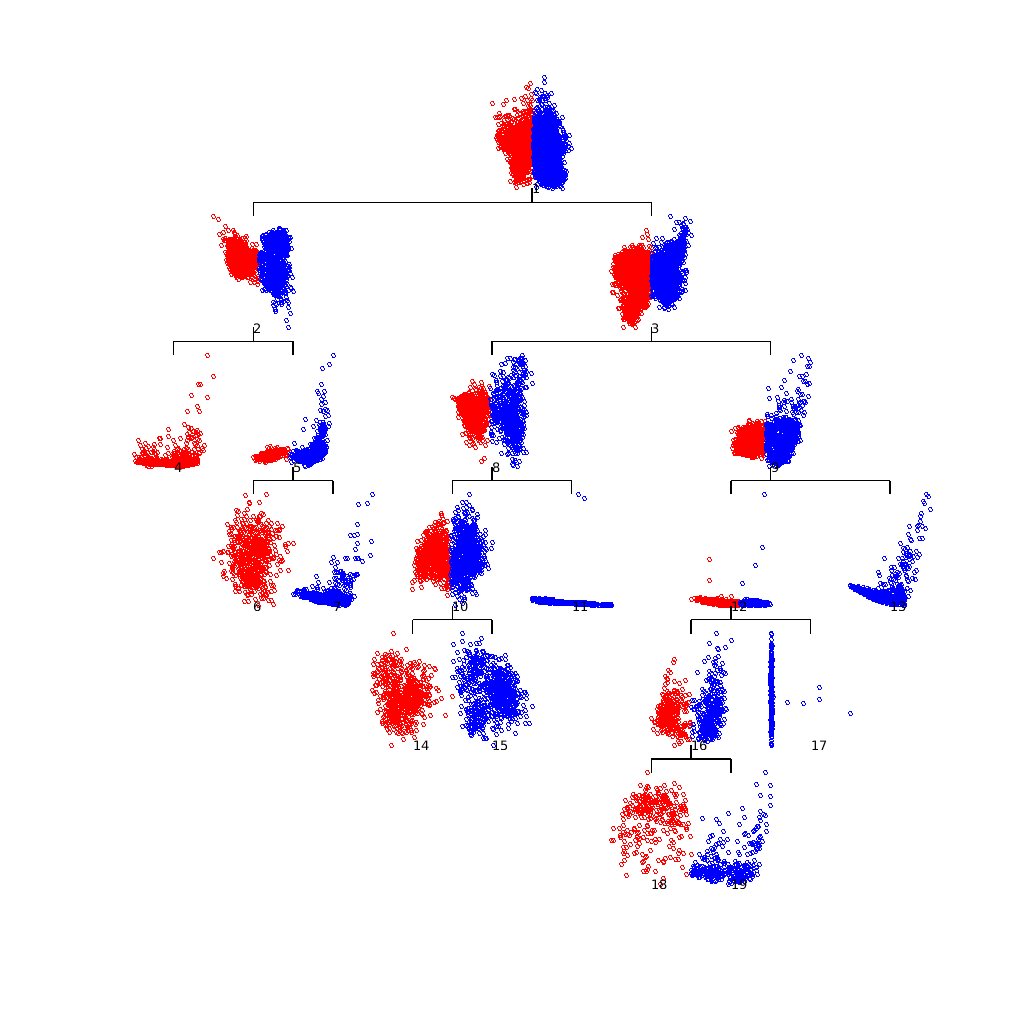
\includegraphics[scale=0.3]{figures/ncut1.png}
%}
%
%\subfigure[Node 3]{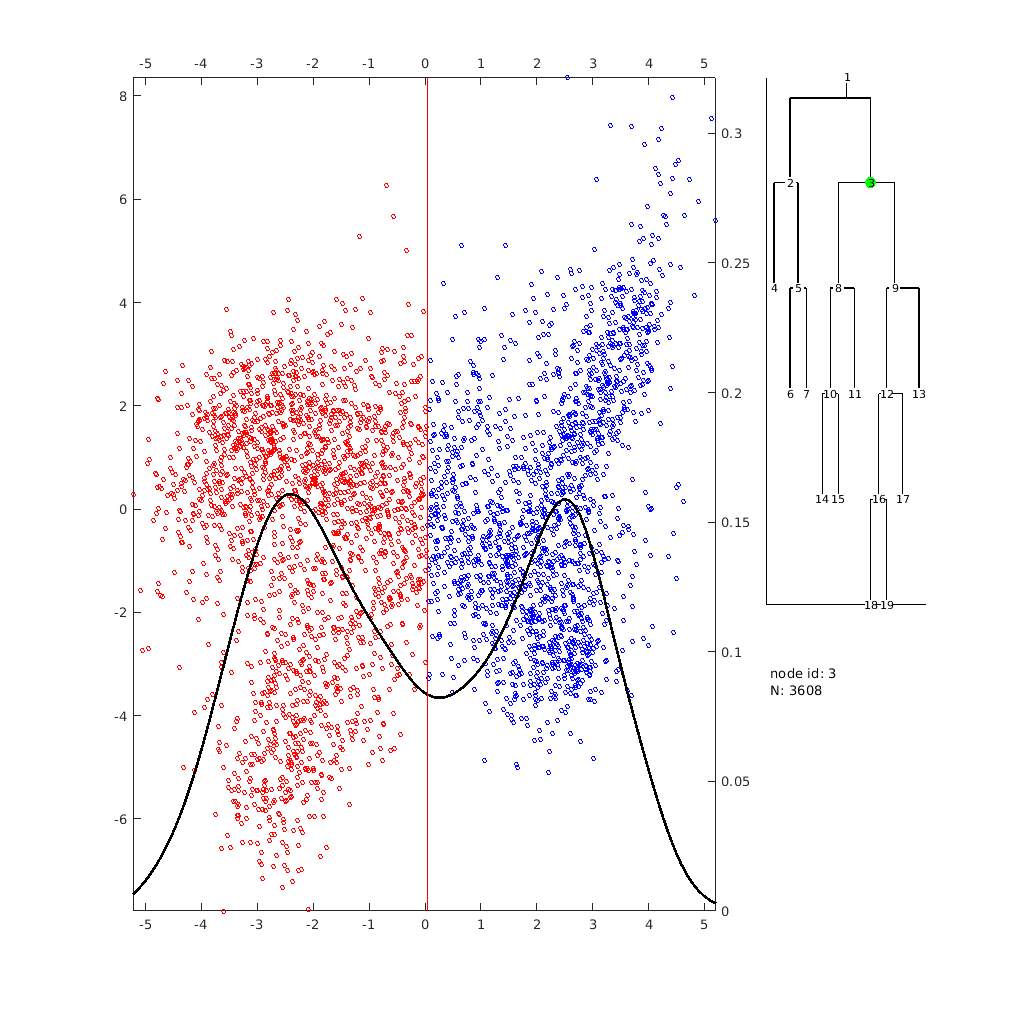
\includegraphics[scale=0.3]{figures/ncut2.png}} 
\end{center}
%
\end{latexonly}
%
\begin{htmlonly}
%
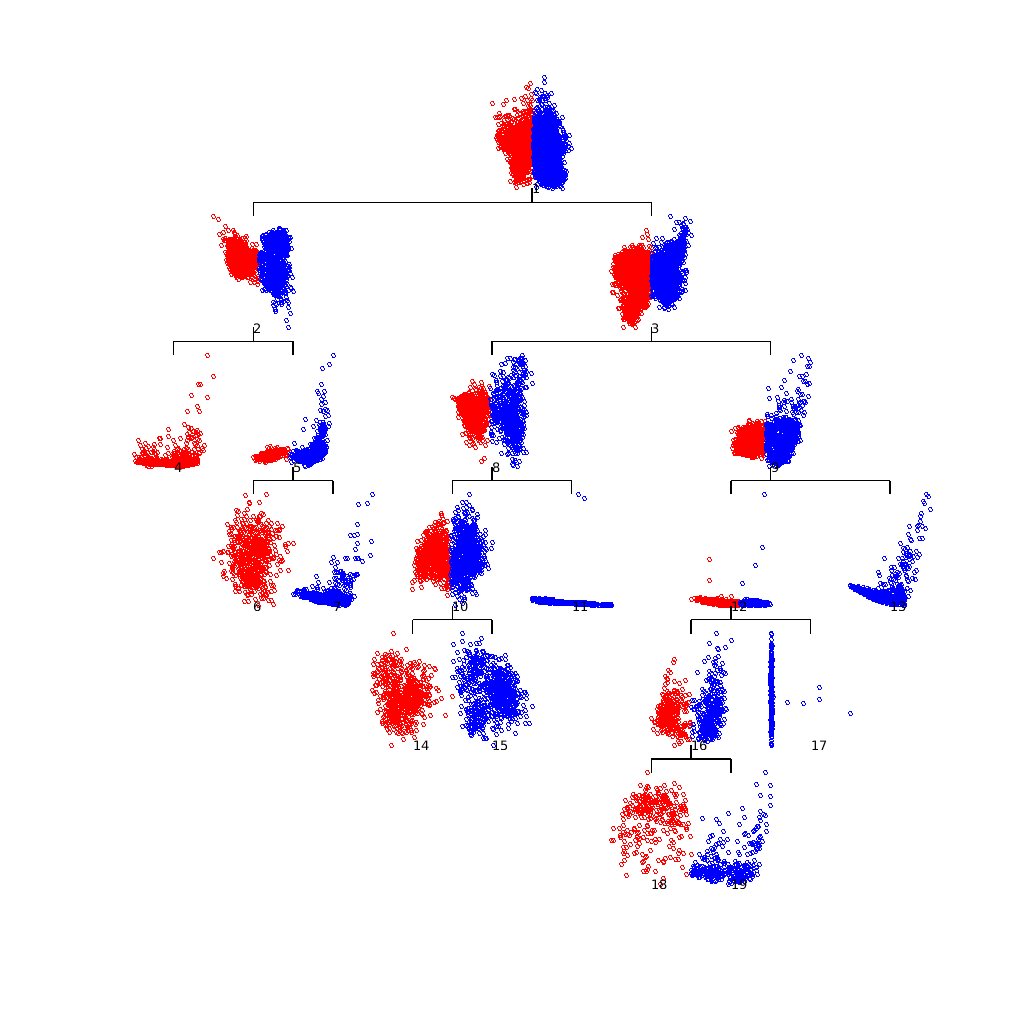
\includegraphics[scale=0.7]{figures/ncut1.png}
%
%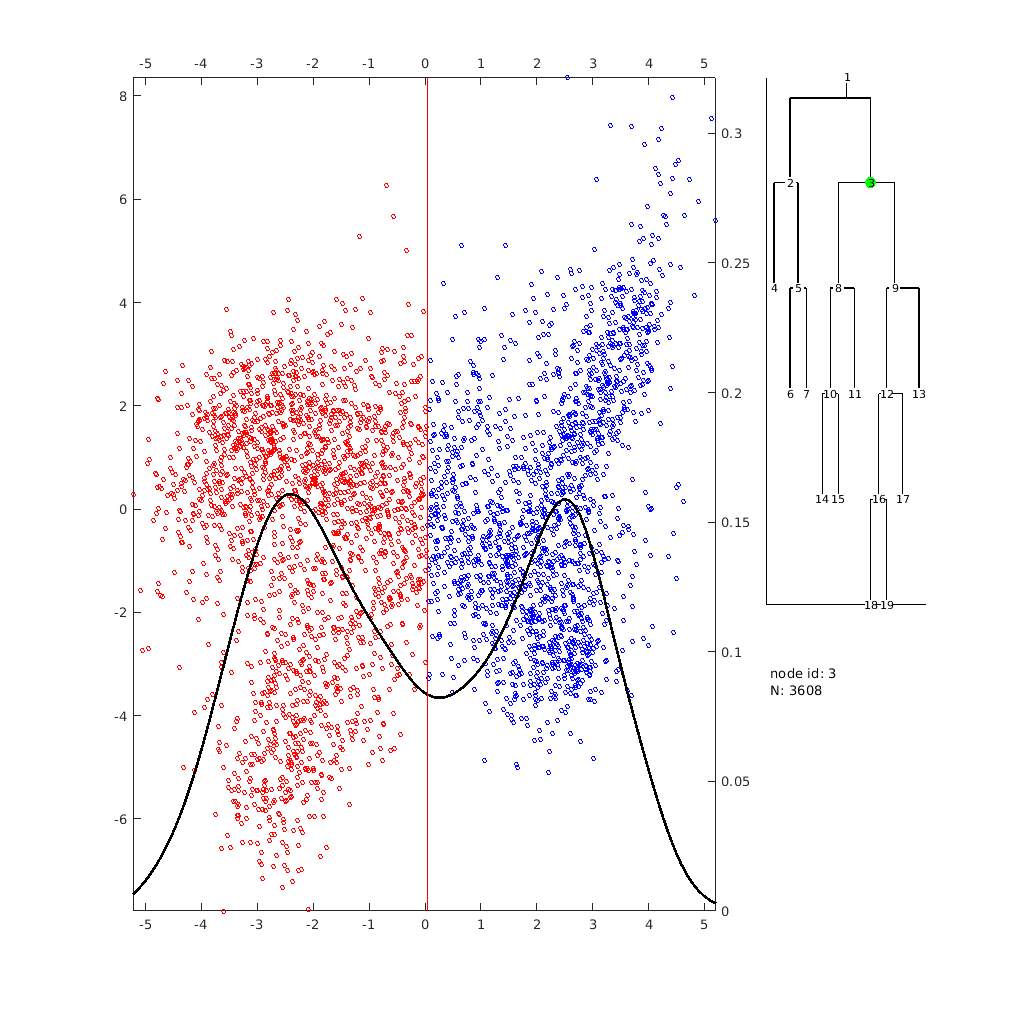
\includegraphics[scale=0.7]{figures/ncut2.png}} 
%
\end{htmlonly}
%
\caption{Cluster hierarchy obtained from NCUTDC using default parameter settings}
%
\label{fig:ncut1}
\end{figure}
%
%
%To improve the clustering model we consider alternative partitions for the data
%subset (cluster) in node 3 of the above model.
%%
%To this end we first must prune the tree at this node, so that node~3 becomes a
%leaf. Then we use the {\tt split} method of the {\tt ctree} class and specify
%alternative initialisations of the projection pursuit algorithm to see if a
%more appropriate partition can be obtained. 
%%
%NCUTDC uses the first principal component as the default initial projection
%vector. In the code below we initialise with the second and third principal
%components and compare the resulting hyperplanes.
%
%\begin{verbatim}
%>> % Prune tree at node 3
%>> t6 = prune(t5,3);
%>> % If you want to verify the output: plot(t6)
%>> 
%>> % Initialise to 2nd PC
%>> t7 = split(t6, 3, 'v0', @(x,p)(pcacomp(x,2)));
%>> nplot(t7,3)
%>>
%>> % Initialise to 3rd PC
%>> t7 = split(t6, 3, 'v0', @(x,p)(pcacomp(x,2)));
%>> nplot(t7,3)
%\end{verbatim}
%
%
%\begin{figure}
%%
%\begin{latexonly}
%%
%\begin{center}
%\subfigure[2nd PC]{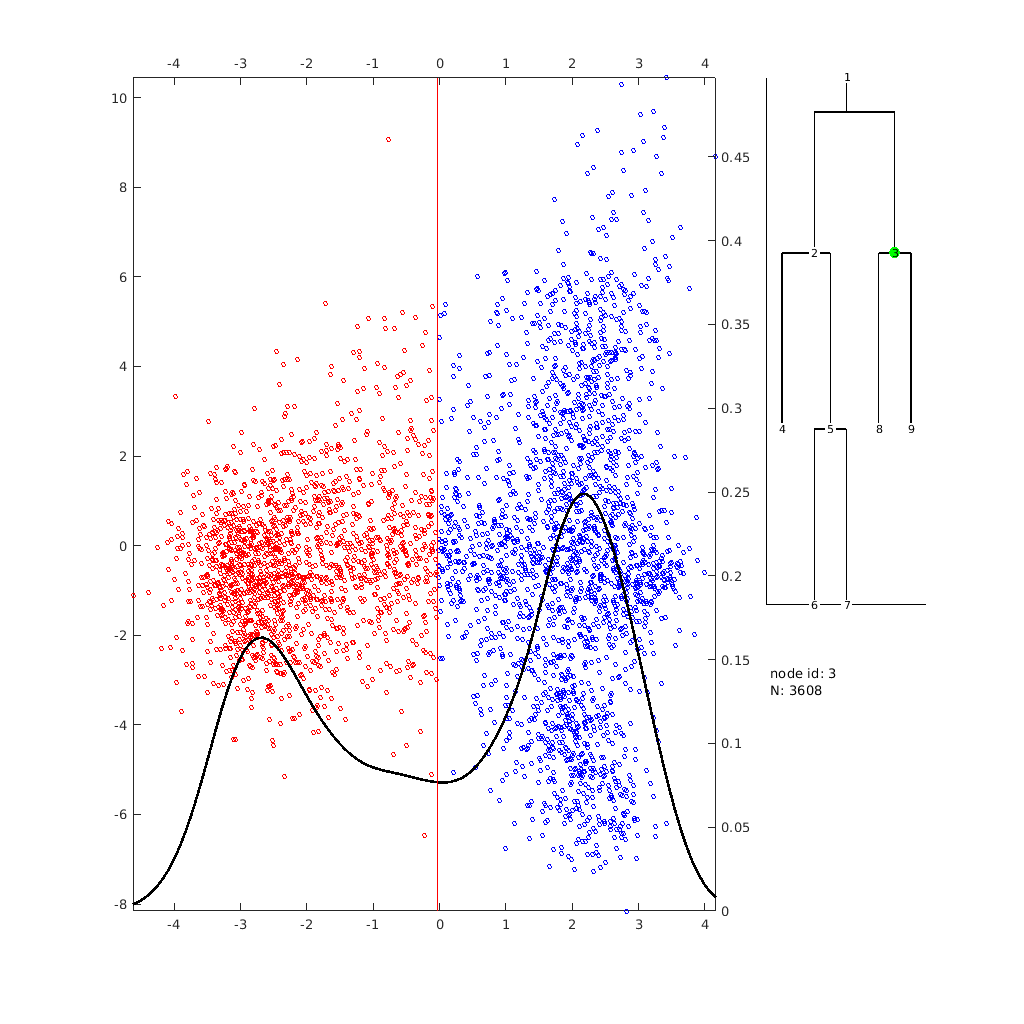
\includegraphics[scale=0.3]{figures/ncut3.png}}
%%
%\subfigure[3rd PC]{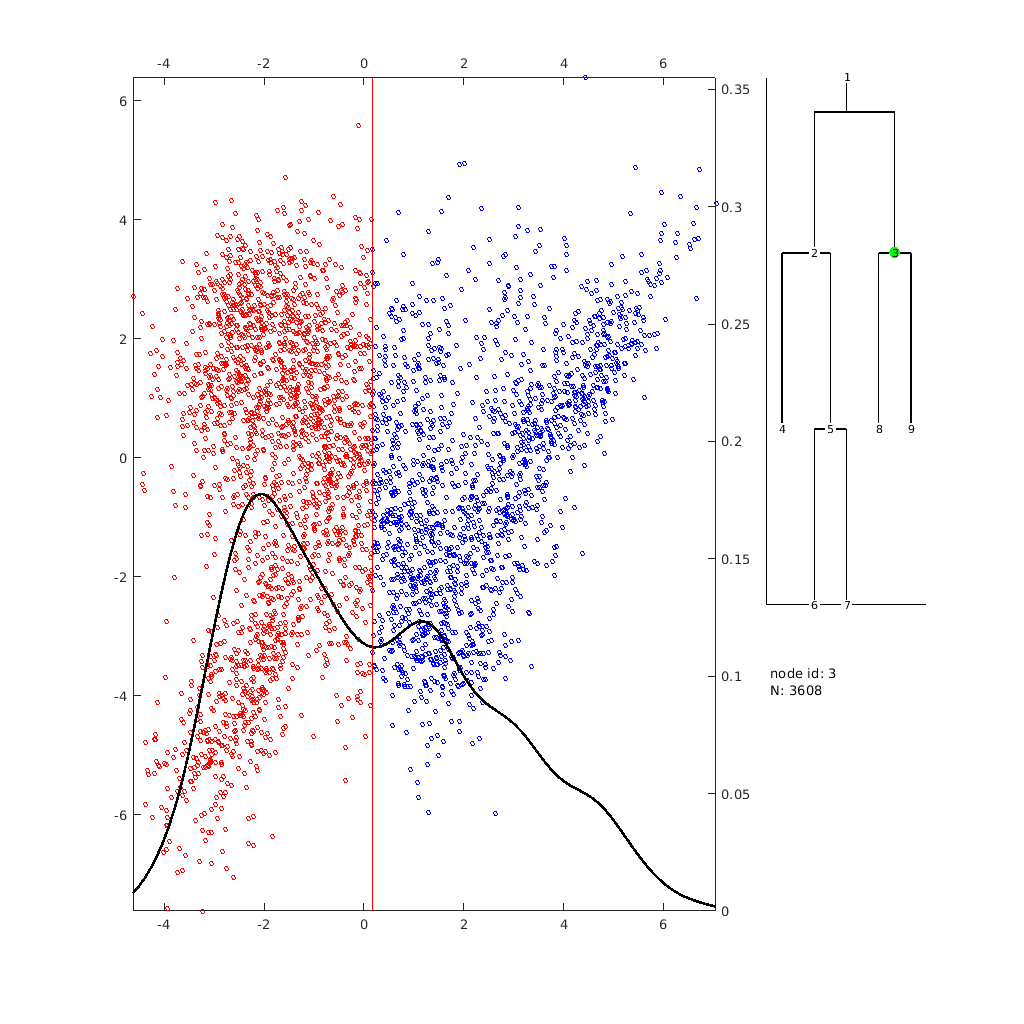
\includegraphics[scale=0.3]{figures/ncut4.png}} 
%\end{center}
%%
%\end{latexonly}
%%
%\begin{htmlonly}
%%
%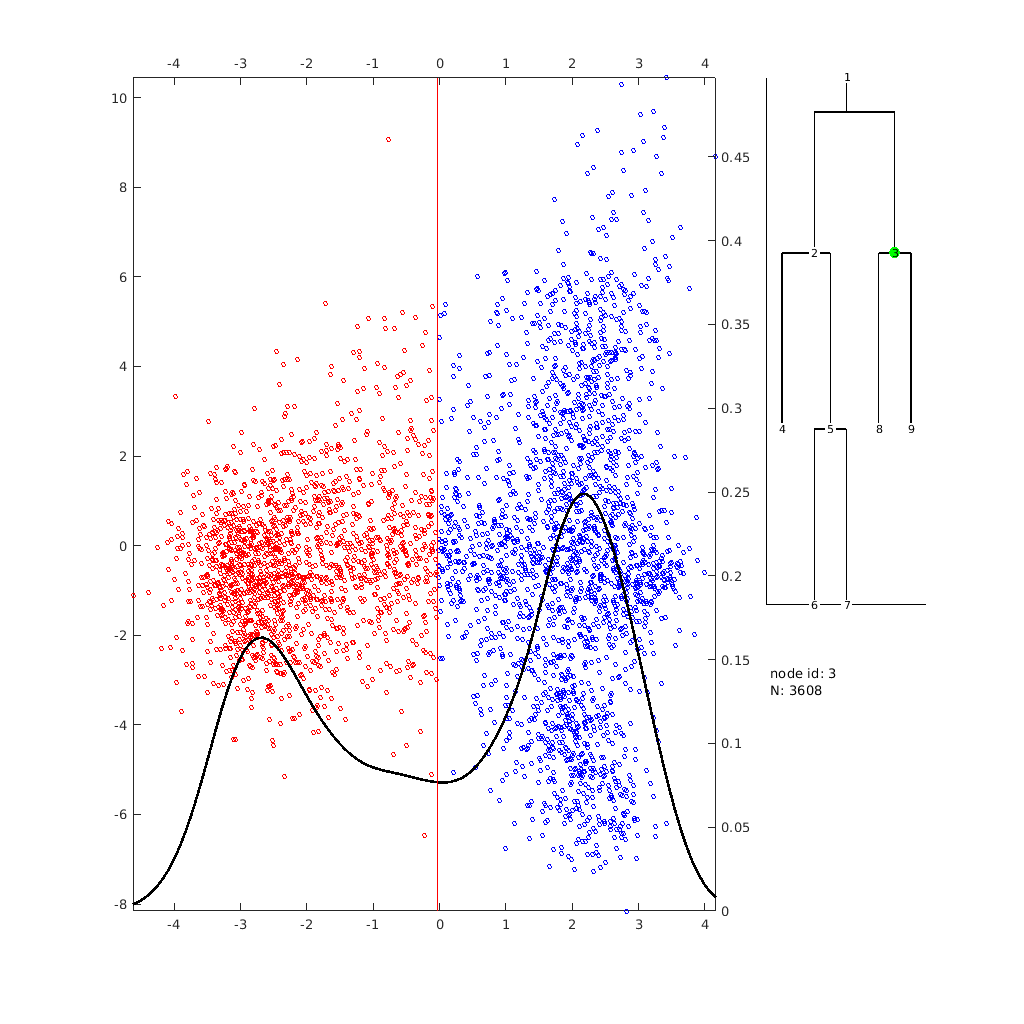
\includegraphics[scale=0.7]{figures/ncut3.png}
%%
%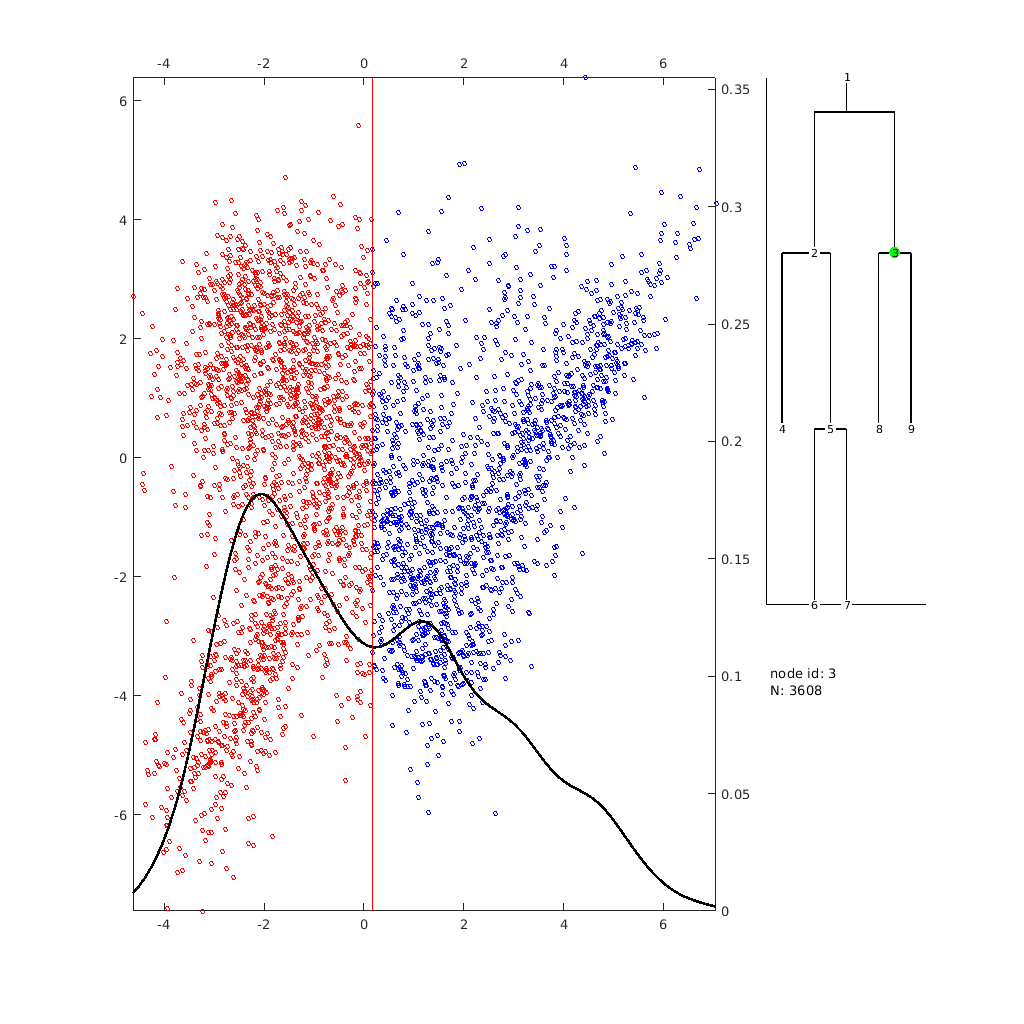
\includegraphics[scale=0.7]{figures/ncut4.png}} 
%%
%\end{htmlonly}
%%
%\caption{Binary partitions at node 3 of previous clustering model after initialising
%the projection pursuit algorithm to the second and third principal component}
%%
%\label{fig:ncut2}
%\end{figure}

\subsection{Minimum Density Divisive Clustering}

The interface to the Minimum Density Divisive Clustering (MCDC) algorithm is
identical to the previous two functions, {\tt mcdc}, and {\tt ncutdc}.
%
For this reason in this section we simply execute the algorithm with the
default settings and in the Section~\ref{sec:valid} we use {\tt mddc} to illustrate how
the user can validate and modify a clustering model through OPC.

\begin{verbatim}
>> [idx6,t6] = mddc(X,10);
>> 
>> % Assess clustering performance
>> cluster_performance(idx6,labels);

ans = 

  struct with fields:

      Purity: 0.8110
         NMI: 0.7716
     AdjRand: 0.7054
    Vmeasure: 0.7716

\end{verbatim}


\section{Spectral Clustering}

In this section we describe two algorithms that attempt to identify the optimal
linear subspace to perform spectral clustering: Dimensionality Reduction for
Spectral Clustering (DRSC), and Spectral Clustering Projection Pursuit (which
to retain the naming conventions in OPC we call Spectral Clustering Projection
Pursuit Divisive Clustering, SCPPDC).
%
Both are gradient-based algorithms that aim to minimise eigenvalue(s) of the
normalised graph Laplacian.
%
Unlike the divisive clustering algorithms discussed in previous sections
the two methods presented in this section are not limited to
one-dimensional projections and can be applied for any choice of the
dimensionality of the projection space,~$q$.
%
This enables these methods to identify clusters whose convex hulls
are not linearly separable.



The Dimensionality Reduction for Spectral Clustering (DRSC)~\cite{NiuDJ2011}
algorithm is a partitioning algorithm. DRSC attempts to identify the projection
matrix~$V$ such that, after the data is projected onto~$V$, the sum of
the $k$ smallest eigenvalues of the normalised graph Laplacian matrix
(computed from the projected data) is minimised.
%
The SCPPDC~\cite{HofmeyrPE2018} iteratively bi-partitions the data by seeking
the two-dimensional linear subspace that minimises the second smallest
eigenvalue of the normalised graph Laplacian (computed from the projected
data).
%
A two dimensional projection is used as this is the smallest dimensionality at
which non-convex clusters can be correctly identified.
%
Although the two methods share a common objective there are significant
differences in how the optimisation is performed. 


Both DRSC and SCPPDC are computationally very expensive, because each function evaluation involves
the computation of the similarity matrix,~$\mathcal{O}(n^2)$, and its eigen-decomposition,
$\mathcal{O}(n^3)$.
%
The gradient ascent scheme for DRSC optimises each column vector
of~$V$ separately, which increases the computational cost by a factor of~$q$.
%
%To render the algorithm practical SCPPDC pre-processes the data through
%micro-clustering. A detailed discussion of the approximation properties of
%using micro-clusters rather than the original data, as well as a sensitivity
%study of the performance of this algorithm with respect to the number of
%micro-clusters is provided in~\cite{HofmeyrPE2018}.
%


\subsection{Dimensionality Reduction for Spectral Clustering}

We will pre-process the data by micro-clustering before applying DRSC so that
the algorithm terminates within a reasonable time.
%
Micro-clustering~\cite{Zhang1996} is effectively $k$-means clustering using
a value of~$k$ that is much larger than the expected number of clusters in
the data.
%
%The second output argument is the number of observations allocated to each
%micro-cluster, and is required by SCPPDC.
%
We will use 200~micro-clusters as recommended for SCPPDC to render the results
of the two algorithms comparable.
%
No recommendation about the scale parameter, $\sigma$, is provided for DRSC. It
is instead suggested to select $\sigma$ through cross--validation using as
performance measure the mean-squared error from the $k$-means step (last step of
spectral clustering).
%
This approach is computationally very expensive. Instead at present we use
the bandwidth selection rule suggested in~\cite{HofmeyrPE2018}, and implemented
in the function {\tt scpp\_def\_sigma}.
%
Finally, the dimensionality of the projection space, $q$, needs to be set.
Following~\cite{NiuDJ2011}, the default setting for~$q$ in {\tt drsc} is
$q=k-1$. We initialise DRSC using the first $k-1$ principal component vectors,
rather than a set of random orthonormal vectors.
We have found that this initialisation improves performance considerably
in the vast majority of cases.
%
The user can modify this parameter specifying the optional argument {\tt v0}. Since
DRSC is not a partitioning algorithm, {\tt v0} can be specified either as a function
handle (as before), or as a projection matrix (which is not allowed for
divisive algorithms).
%
When the optional argument {\tt v0} is set $q$~is determined by the
number of columns of the initial projection matrix.

\begin{verbatim}
>> % micro-clustering
>> [d2c,centroids] = kmeans(X,200); 
>>
>> % Set scale parameter for Gaussian kernel
>> % to default value recommended for SCPPDC
>> sigma = scpp_def_sigma(X);
>> 
>> % Execute drsc
>> [idx7,W,fval,sumD] = drsc(centroids,10,sigma);
>>
>> % Assign cluster labels to observations using
>> % the cluster labels of the micro-clusters
>> idx7 = reverse_assign(idx7, d2c);
>>
>> cluster_performance(idx7, labels);

ans = 

  struct with fields:

      Purity: 0.1283
         NMI: 0.0802
     AdjRand: 6.1091e-04
    Vmeasure: 0.0497

\end{verbatim}

\noindent
%
DRSC terminates after exhausting the maximum number of iterations (the default
value for which 50) without converging. A plot of the projection index after
each complete pass over all the columns of~$V$ (contained in the third
output argument {\tt fval}) indicates that the algorithm is not monotonically
improving the objective function.
%
The clustering quality of the identified solution is also poor.


\subsection{Spectral Clustering Projection Pursuit Divisive Clustering}

Next we apply the SCPPDC algorithm on the {\tt optidigits} dataset. The syntax
for this divisive hierarchical algorithm is identical to the previous
algorithms. The function {\tt scppdc} uses all the default values recommended
in~\cite{HofmeyrPE2018}, and the user need only specify the data matrix and the
number of clusters. 
%
A critical parameter for this algorithm (as for all
spectral clustering methods) is the choice of the scale parameter, $\sigma$, of
the Gaussian kernel that is used to compute pairwise similarities.
%
By default this parameter is set through the function {\tt scpp\_def\_sigma}.
The user can modify this by setting the optional argument {\tt sigma}
to a function handle. The associated function must accept as
arguments a data matrix and a structured array containing the parameters
of the algorithm.
%
Also very influential is the choice of the initial projection matrix.
In {\tt scppdc} the projection matrix is initialised to the first two principal
components of the cluster being split. 
The user can modify this by specifying the optional
argument {\tt v0}. As in all divisive hierarchical algorithms, {\tt v0} must
be a handle to a
function that returns a projection matrix and accepts as inputs
the data matrix and a structured array containing all the parameters
of the algorithm.

\begin{verbatim}
>> [idx8, t8] = scppdc(X,10);
Clusters: 1 2 3 4 5 6 7 8 9 10
>> % Visualisation
>> plot(t8)
>> plot(t8,labels)
>> % Performance assessment
>> cluster_performance(idx8,labels)

ans = 

  struct with fields:

      Purity: 0.8448
         NMI: 0.7872
     AdjRand: 0.7155
    Vmeasure: 0.7872

\end{verbatim}

\begin{figure}
%
\begin{latexonly}
%
\subfigure[Labels unspecified]{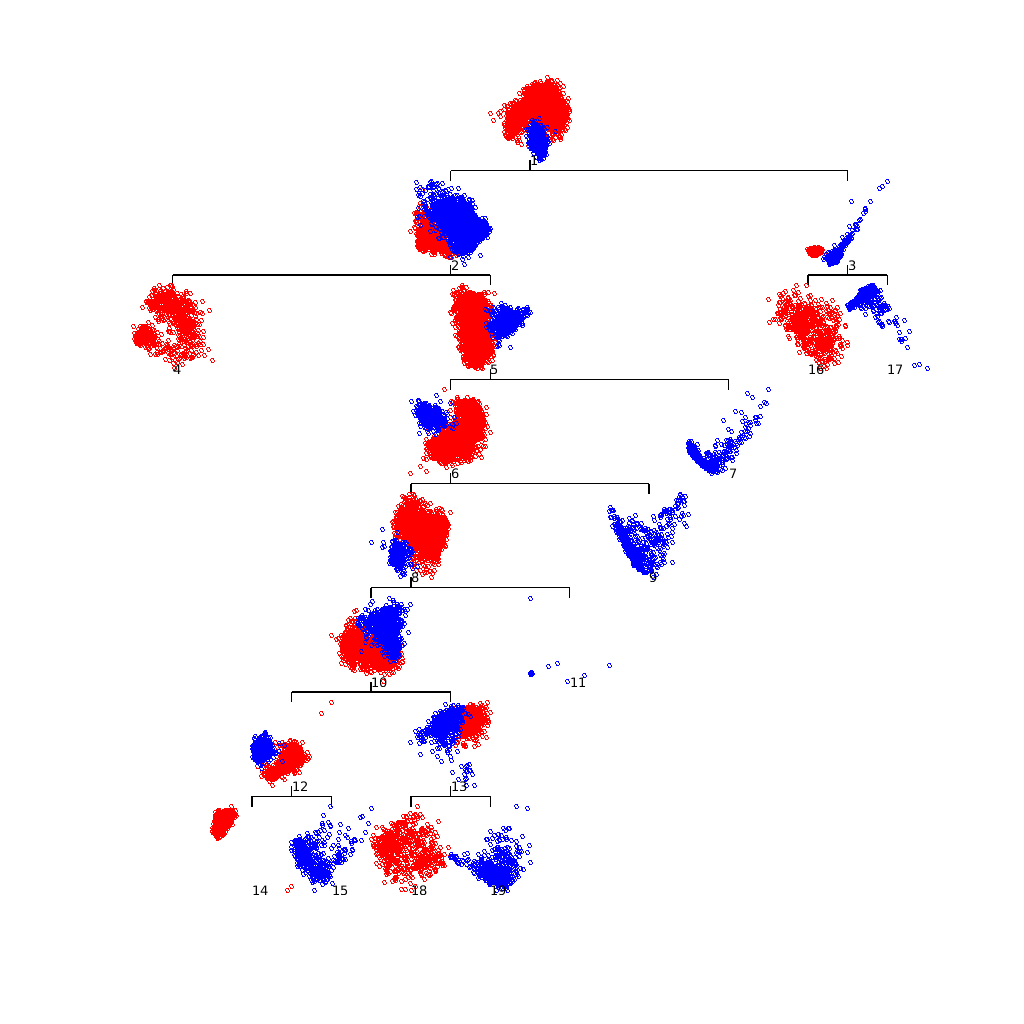
\includegraphics[scale=0.3]{figures/scpp1.png}} 
%
\subfigure[Labels specified]{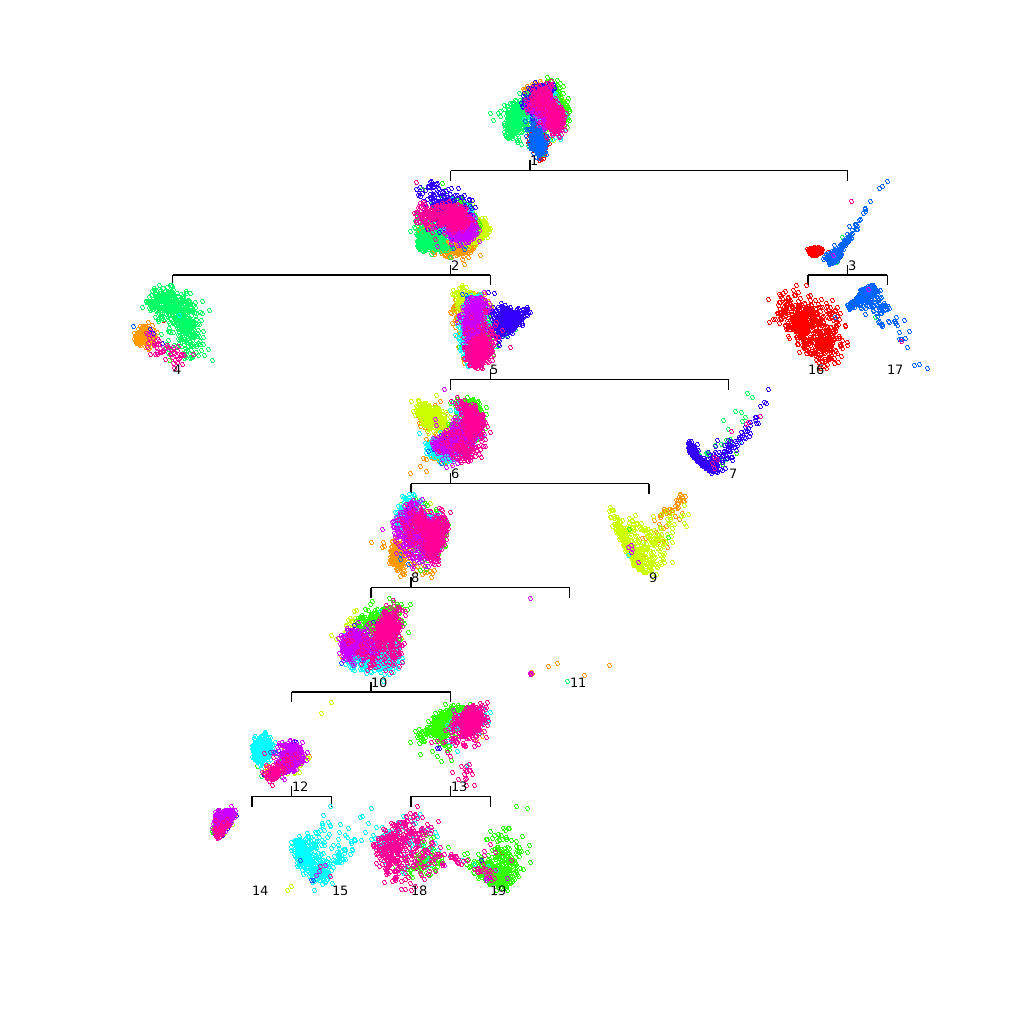
\includegraphics[scale=0.3]{figures/scpp2.png}} 
%
\end{latexonly}
%
\begin{htmlonly}
%
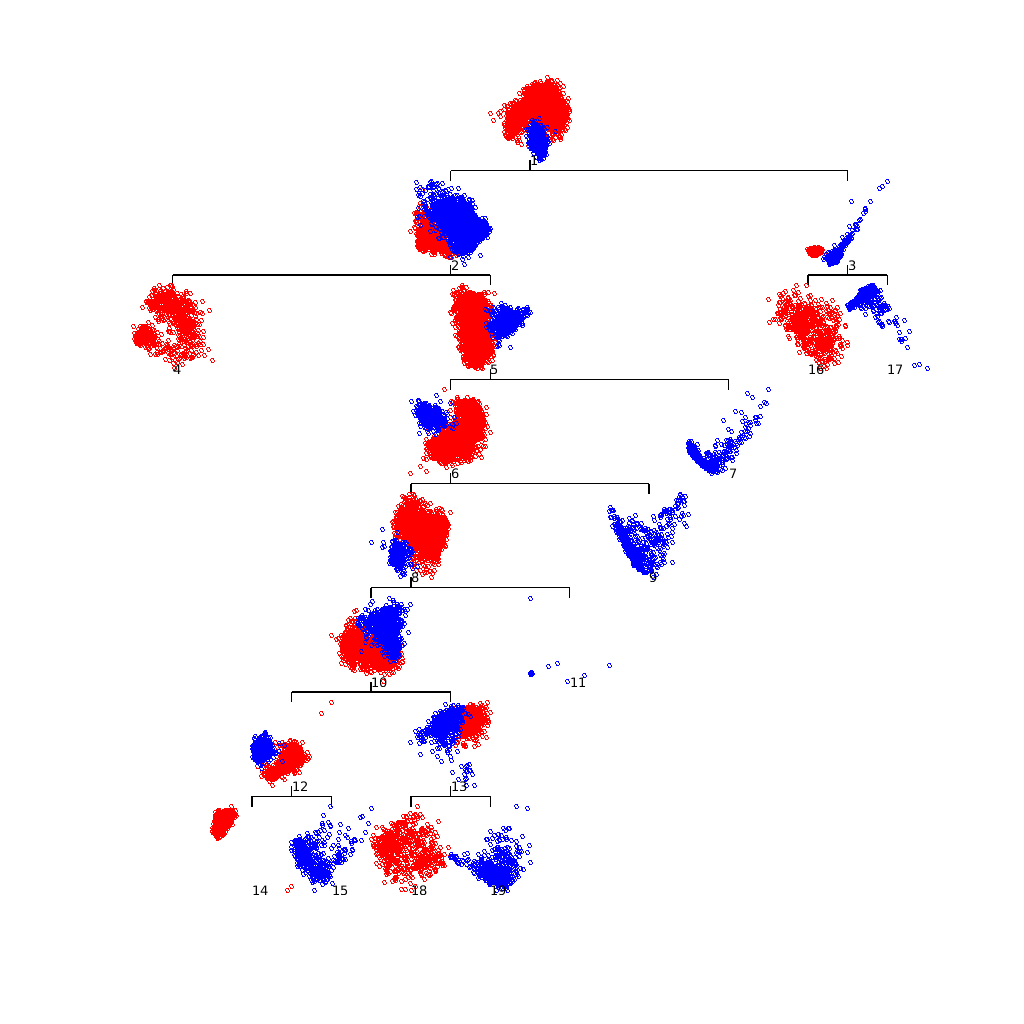
\includegraphics[scale=0.7]{figures/scpp1.png}} 
%
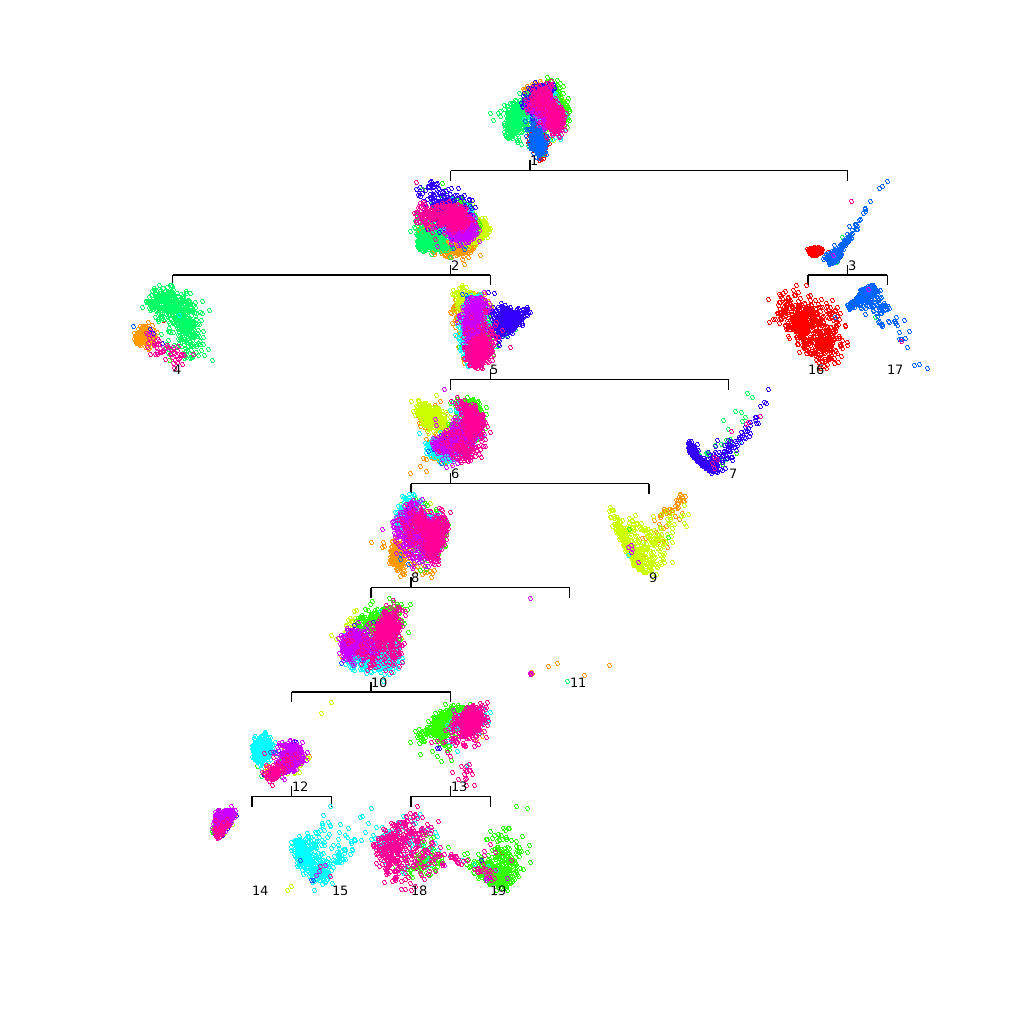
\includegraphics[scale=0.7]{figures/scpp2.png}} 
%
\end{htmlonly}
%
\caption{Cluster hierarchy produced by {\tt scppdc} without and with the specification of labels}
%
\label{fig:scpp1}
\end{figure}


\noindent
%
Figure~\ref{fig:scpp1} illustrates the cluster hierarchy produced by {\tt
scppdc}.
%
%Notice that the algorithm separates effectively at least one non-convex
%cluster from the rest at each partition. 
%
The only leaf node (cluster) that appears to contain more than one clusters is
the node with number~4. The second sub-figure in Figure~\ref{fig:scpp1}
verifies that this impression is correct. It is also clear that the ability to
separate non-convex clusters in the two-dimensional projection space
enhances the performance of this algorithm.
%
This is verified by the cluster performance measures. SCPPDC achieves the
highest performance out of all the considered methods on this dataset, and
importantly improves substantially over spectral clustering applied on the full
dimensional dataset, as well as on data projected onto the first $q$ principal
components.







\chapter{Model Validation and Modification}\label{sec:valid}

In this section we illustrate how to validate and modify a clustering model
produced by any divisive hierarchical clustering algorithm in OPC.
%
For partitioning algorithms, visualisation is straightforward using the
projection matrix. To modify the model produced by a partitioning algorithm the
user needs to modify the optional input arguments, as discussed in the previous
section.
%
Therefore there is little to discuss with respect to the process of visualising
and modifying the output of partitioning algorithms.

In the present example we will use the {\tt optidigits} datasets used in the
previous section, but assume that the actual number of clusters is unknown,
and start with an initial guess of $k=5$.
%
We will use the MDDC algorithm, but the interface we describe is applicable to
all divisive hierarchical clustering methods in OPC.
%
The functions for visualisation, {\tt plot} and {\tt nplot}
have been discussed extensively in the previous
section.
The two main functions for the modification of a clustering hierarchy are
{\tt prune} and {\tt split}, which are methods of the {\tt ctree} class.

\begin{verbatim}
>> load('datasets/optidigits.mat');
>>
>> % Cluster optidigits datasets assuming k=5
>> [idx,t] = mddc(X,5)
>> Visualise cluster hierarchy (plot not shown)
>> plot(t);
>> % Evidence of 3 well separated clusters
>> nplot(t,2);
>> % Hyperplane intersects dense area
>> plot(t,3);
\end{verbatim}

\begin{figure}
%
\begin{latexonly}
%
\begin{center}
%\subfigure[Cluster hierarchy]{ 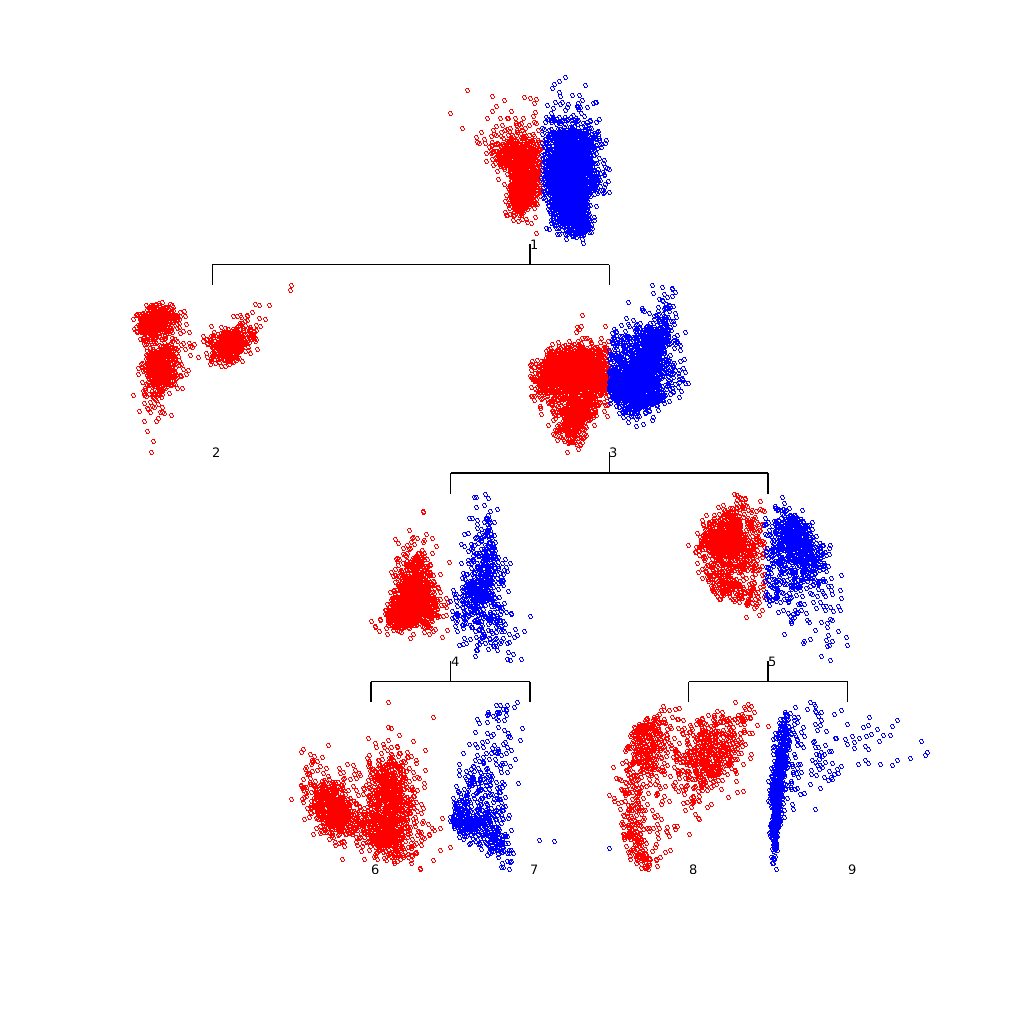
\includegraphics[scale=0.3]{figures/val1.png}}
%
\subfigure[Node 2]{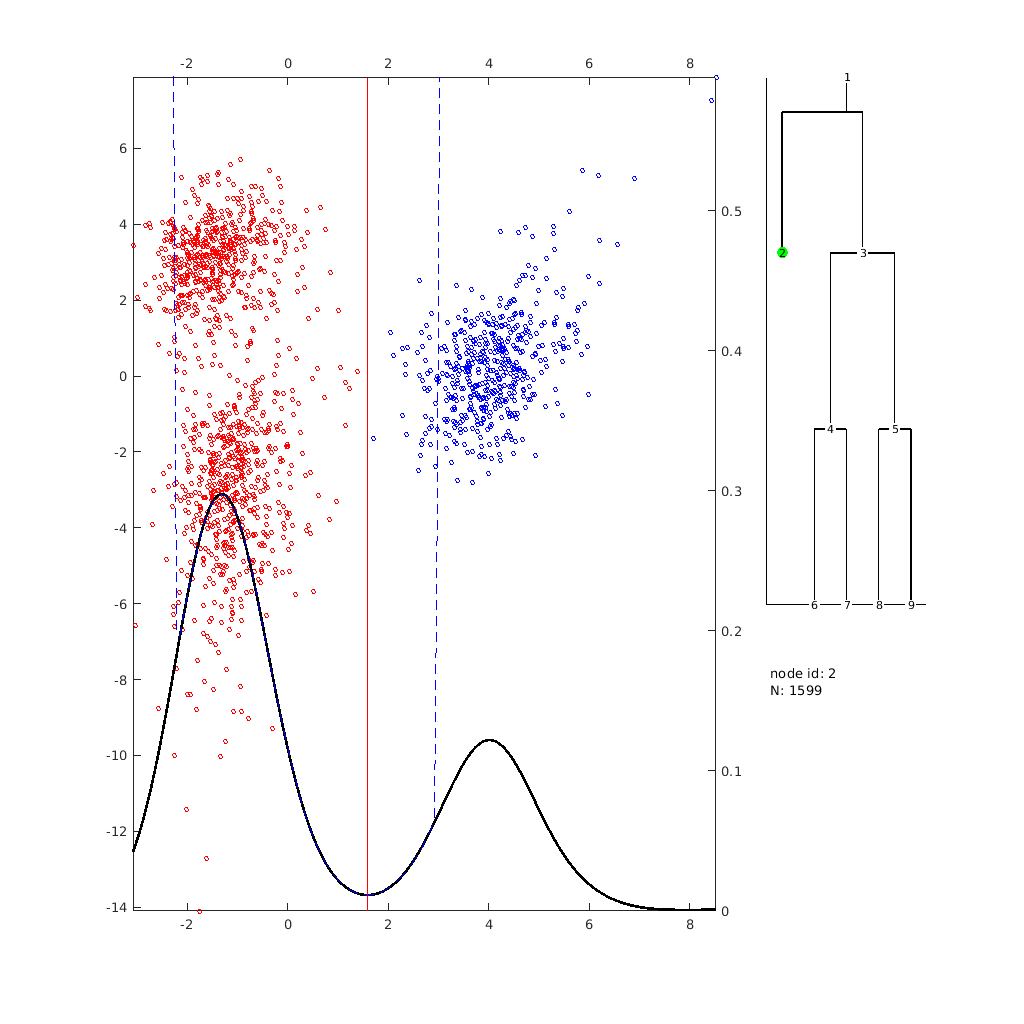
\includegraphics[scale=0.3]{figures/val2.png}} 
%
\subfigure[Node 3]{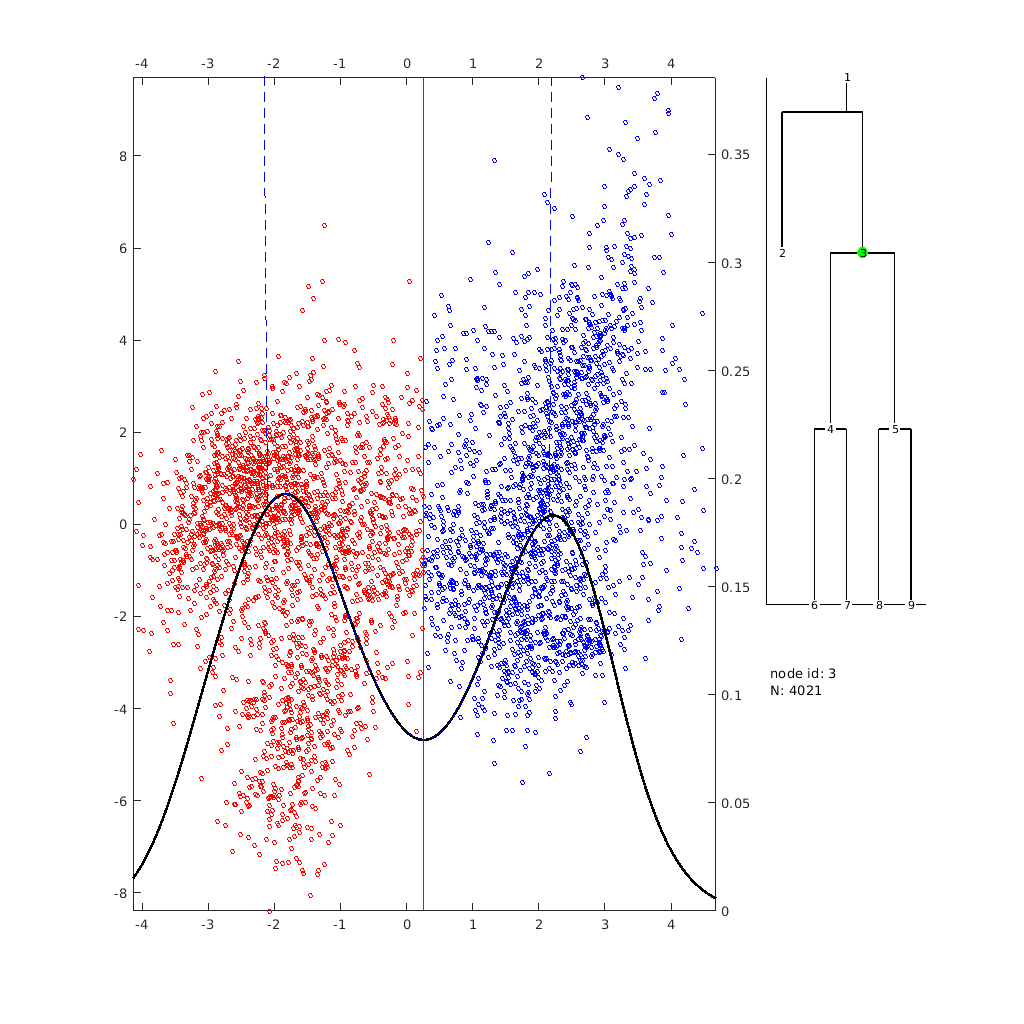
\includegraphics[scale=0.3]{figures/val3.png}} 
%
\end{center}
\end{latexonly}
%
\begin{htmlonly}
%
%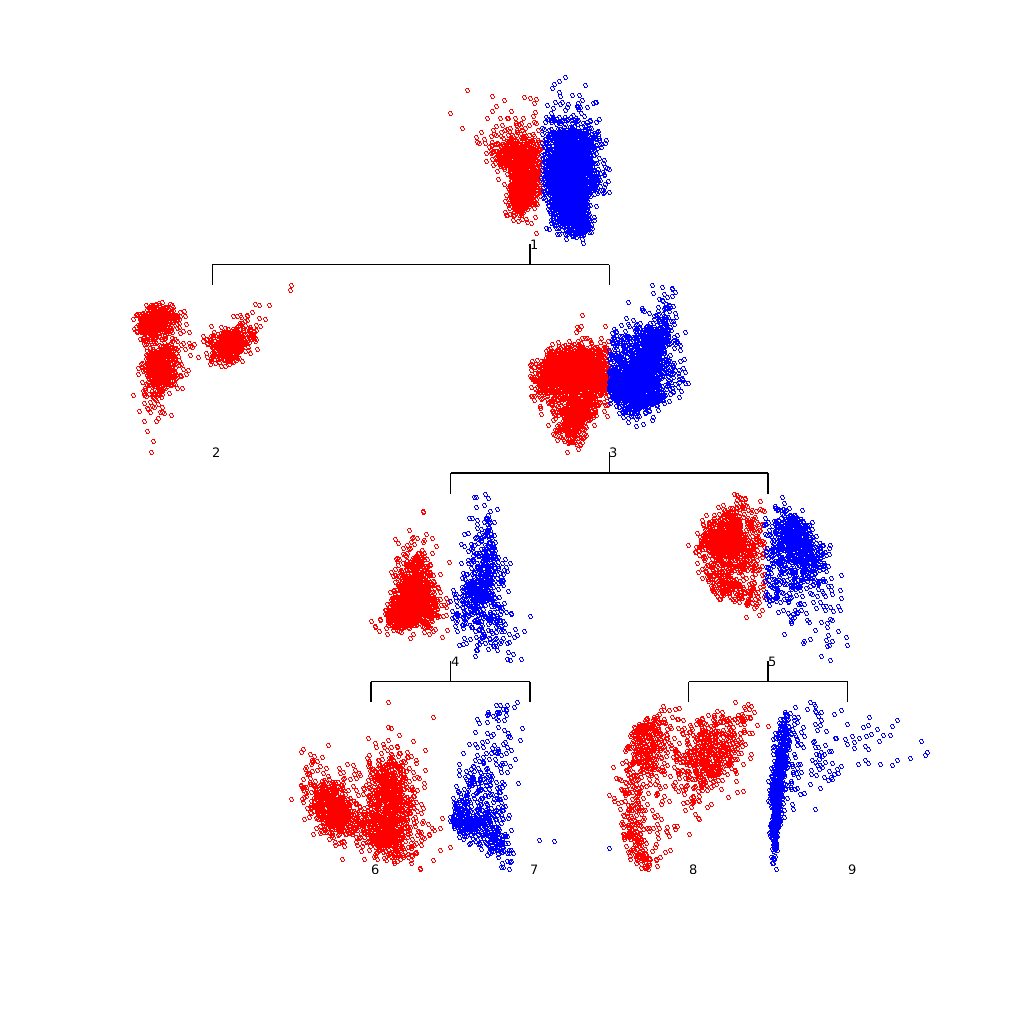
\includegraphics[scale=0.7]{figures/val1.png}} 
%
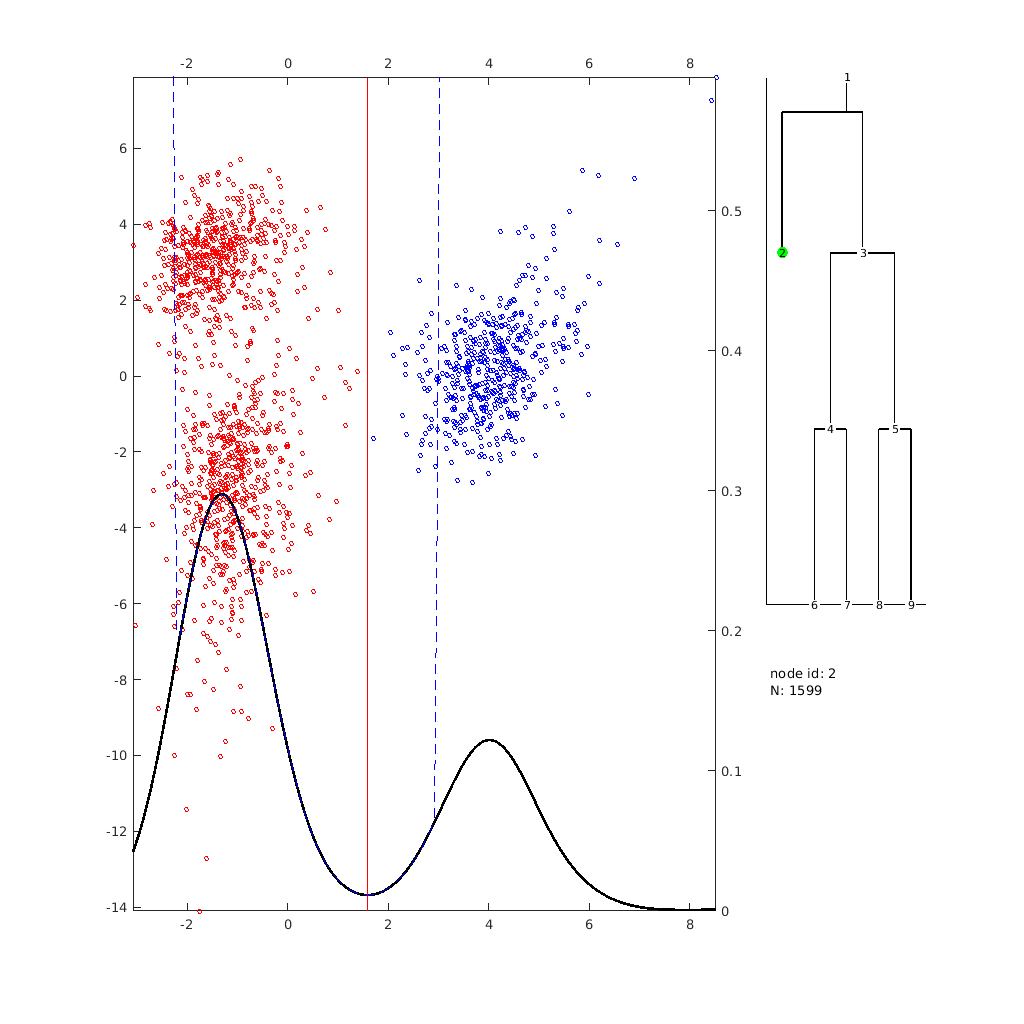
\includegraphics[scale=0.7]{figures/val2.png}} 
%
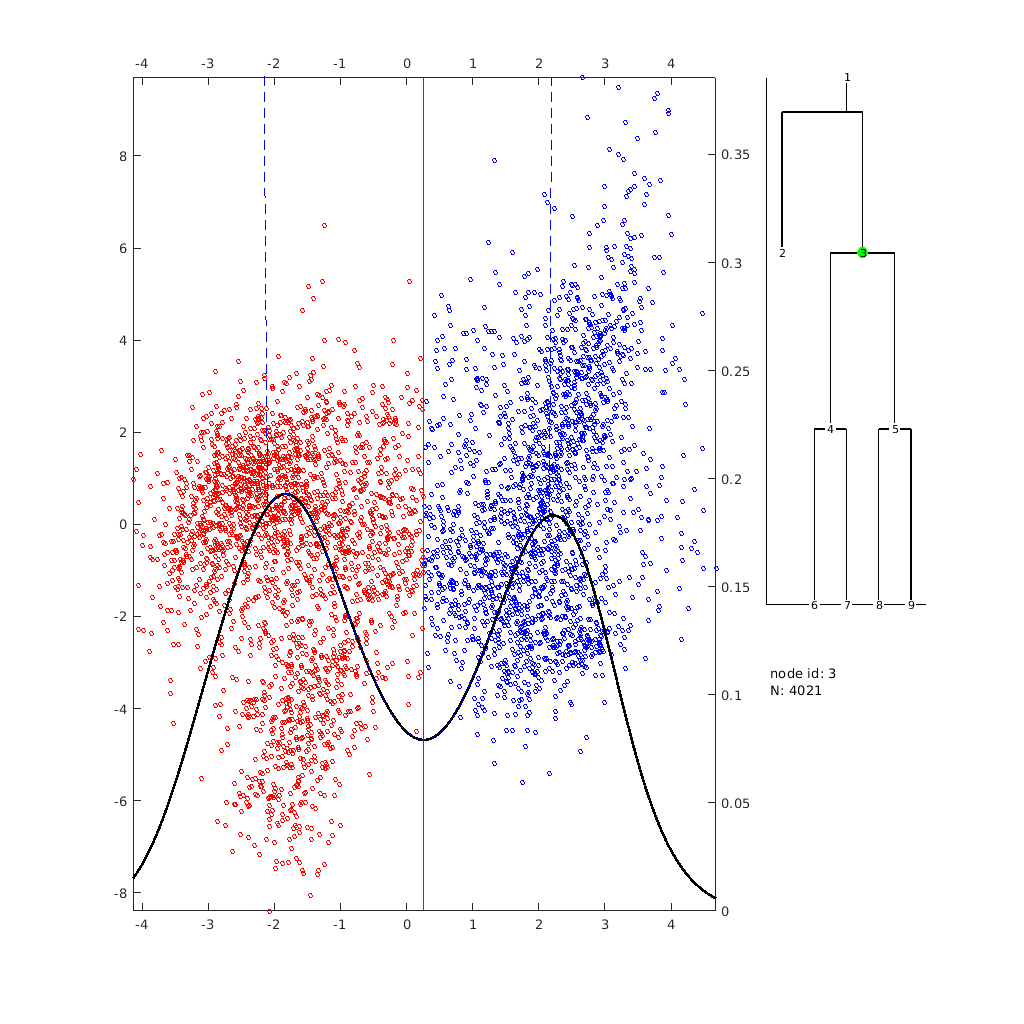
\includegraphics[scale=0.7]{figures/val3.png}} 
%
\end{htmlonly}
%
\caption{Binary partitions at nodes 2 and 3 of initial clustering hierarchy}
%
\label{fig:val1}
\end{figure}
%

\noindent
%
An inspection of the cluster hierarchy (not shown for brevity), and the
hyperplane separators in nodes~2 and~3 in Figure~\ref{fig:val1}, suggests that
the leaf node 2, appears to contain 3 well separated dense clusters, while the
hyperplane in node 3 intersects a dense region.
%
The dashed blue line in Figure~\ref{fig:val1} corresponds to the projection
index for MDH, $f(v)$ defined in Eq.~(\ref{eq:mdh2}).
%
Notice that $f(v)$ is identical to the density estimator within the range
of $\alpha$ standard deviations around the mean; while 
it increases abruptly outside this range. 
%
The definition of the projection index ensures that its minimiser will always
be within $\alpha$ standard deviations of the mean of the data (which in this example is zero).
%
The hyperplane separator for the cluster at node 2 appears to be effectively
separating one of the tree dense clusters.  We can therefore use this
hyperplane to split the cluster at node 2. 
%
This happens when the {\tt split} function is called with no optional
arguments. 
%
An inspection of the new leaf node with number 10 (omitted for brevity),
illustrates that this cluster contains two of the three dense clusters
identified in node~2, and that the MDH for this node separates these
clusters effectively.
%
We therefore split those by calling the {\tt  split} function without
specifying any arguments.


\begin{verbatim}
>> % Split cluster at leaf node 2 using estimated MDH
>> t1 = split(t,2);
>> % Plot omitted for brevity
>> nplot(t1,10);
>> % Split cluster at leaf node 10 using estimated MDH
>> t1 = split(t1,10);
>> % Visualise cluster hierarchy
>> plot(t1);
\end{verbatim}

\noindent
%
We next explore whether the binary partition at node 3 can be improved.
%
To consider alternative hyperplane separators, we first need to
prune the subtree rooted at this node, because the {\tt split} function can
only be applied to a leaf node. Note that after the tree is pruned
the numbers of different nodes can change,
as shown in Figure~\ref{fig:val2}. Node numbers in {\tt ctree} objects
are always consecutive, and represent the order in which nodes were added to the model.

\begin{figure}
%
\begin{latexonly}
%
\begin{center}
%\subfigure[Cluster hierarchy]{ 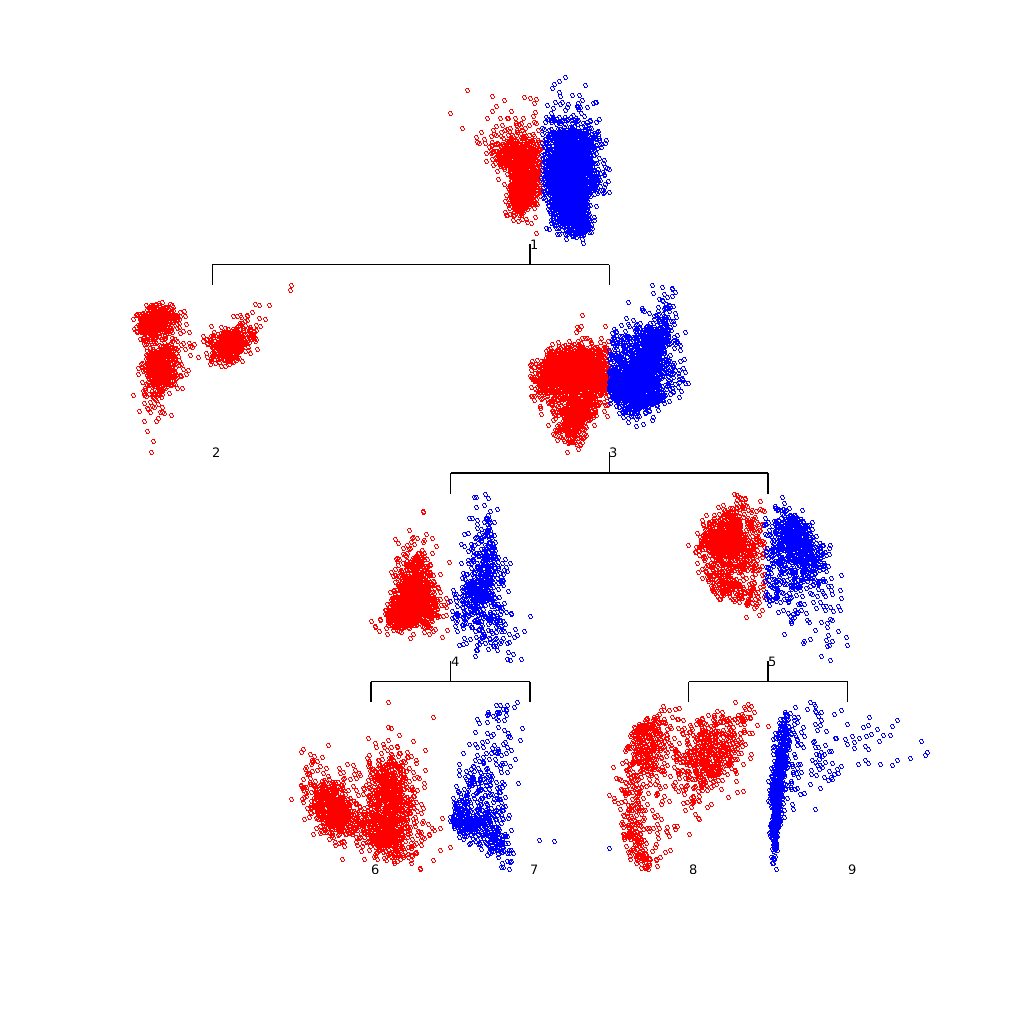
\includegraphics[scale=0.3]{figures/val1.png}}
%
\subfigure[Tree after splitting node 2]{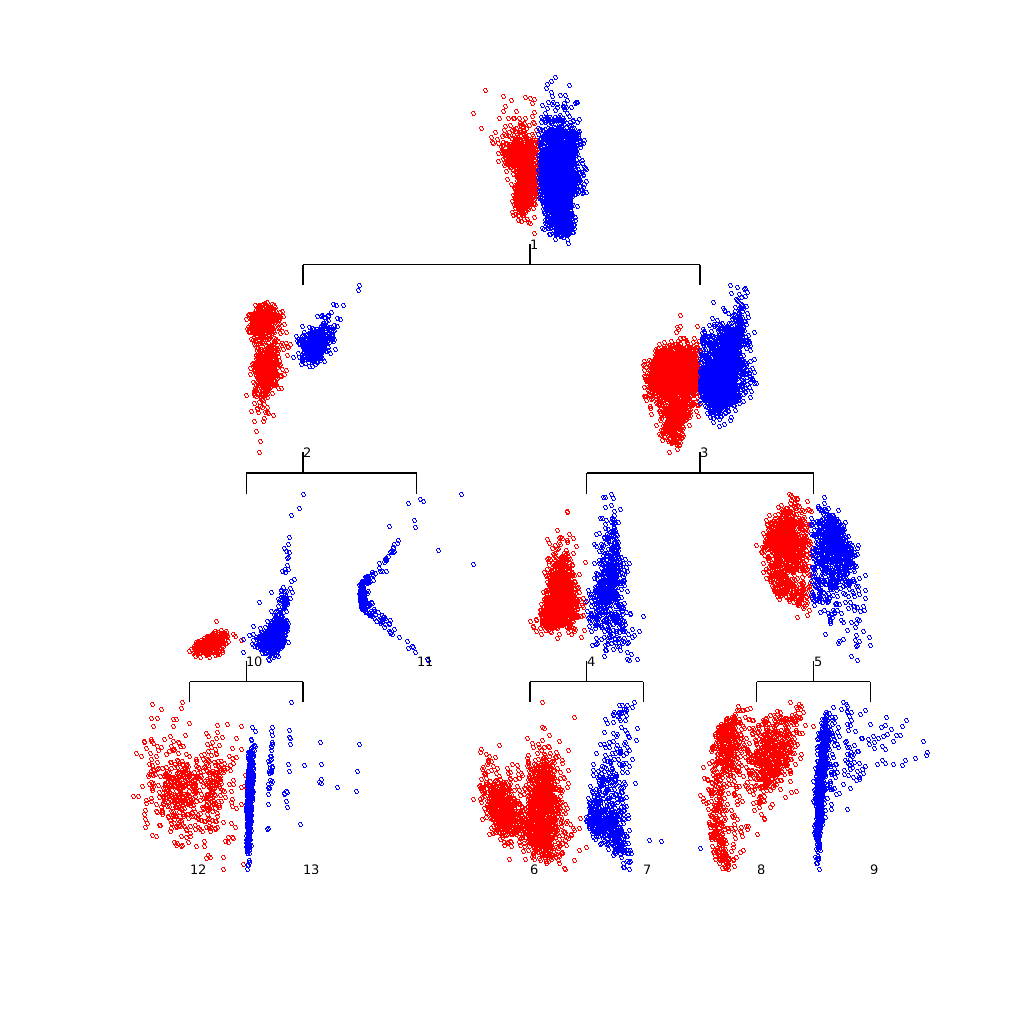
\includegraphics[scale=0.3]{figures/val4.png}} 
%
\subfigure[Tree after pruning node 3]{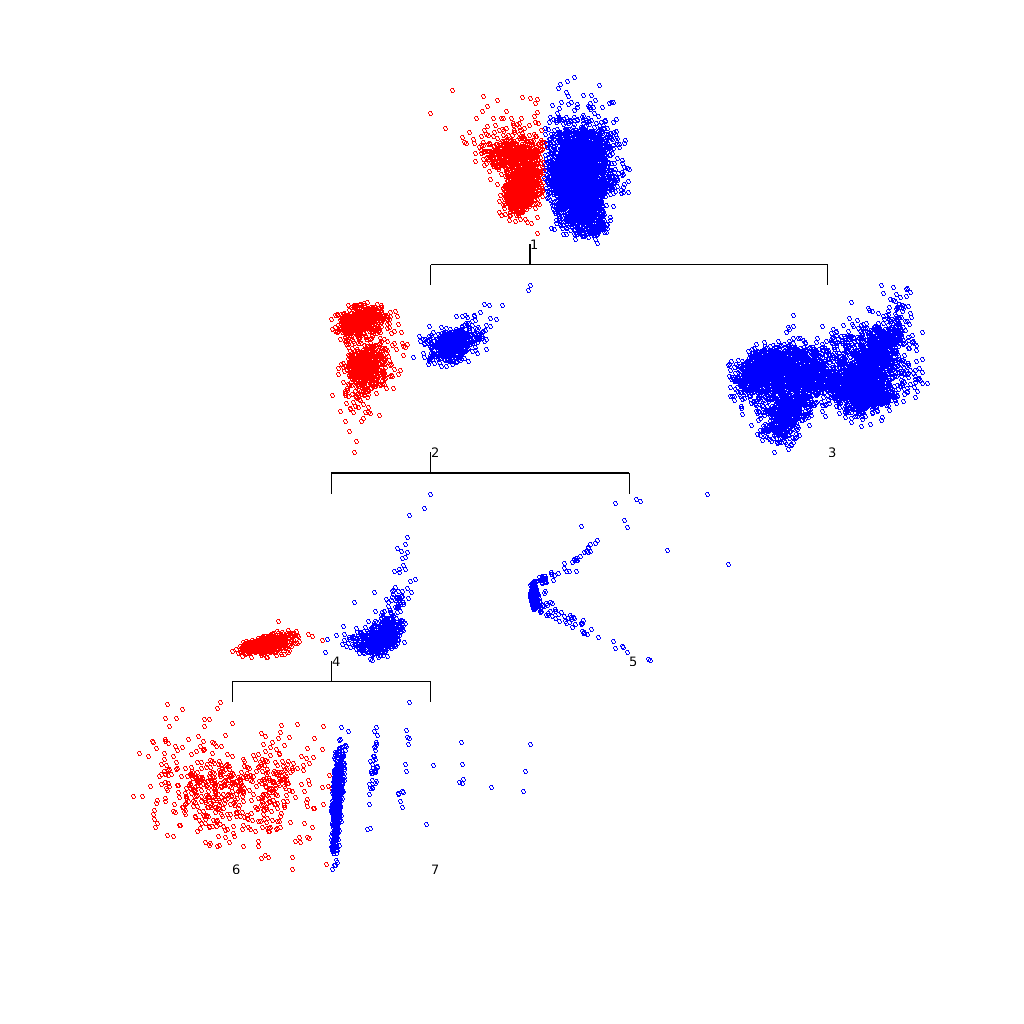
\includegraphics[scale=0.3]{figures/val5.png}} 
%
\end{center}
\end{latexonly}
%
\begin{htmlonly}
%
%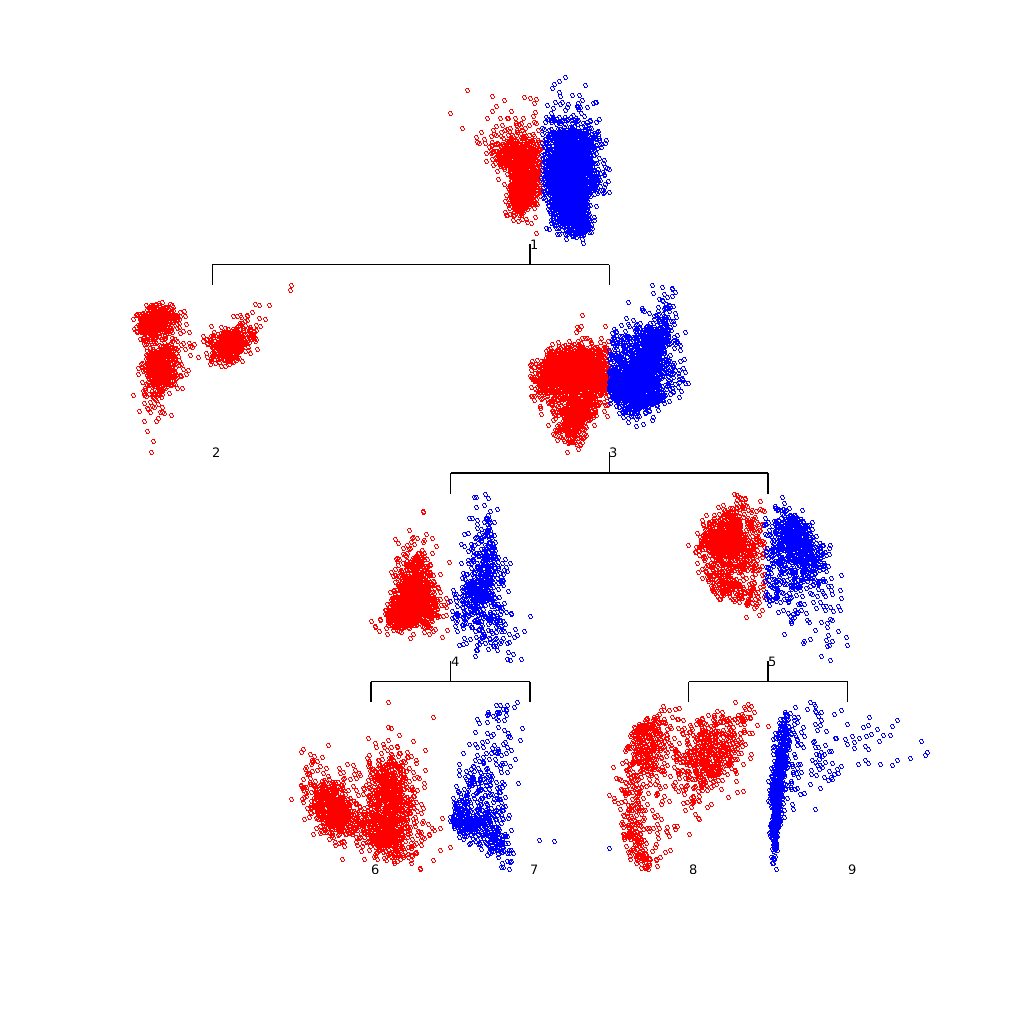
\includegraphics[scale=0.7]{figures/val1.png}} 
%
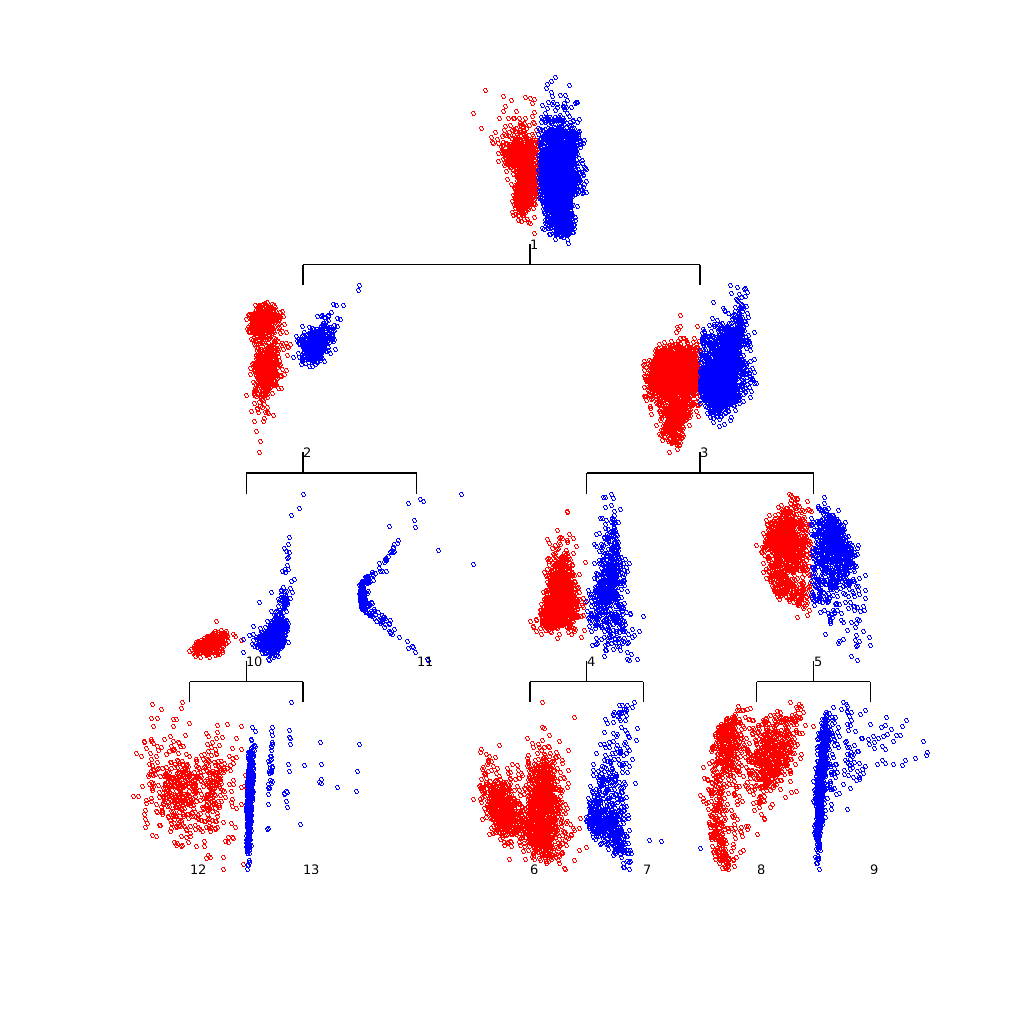
\includegraphics[scale=0.7]{figures/val4.png}} 
%
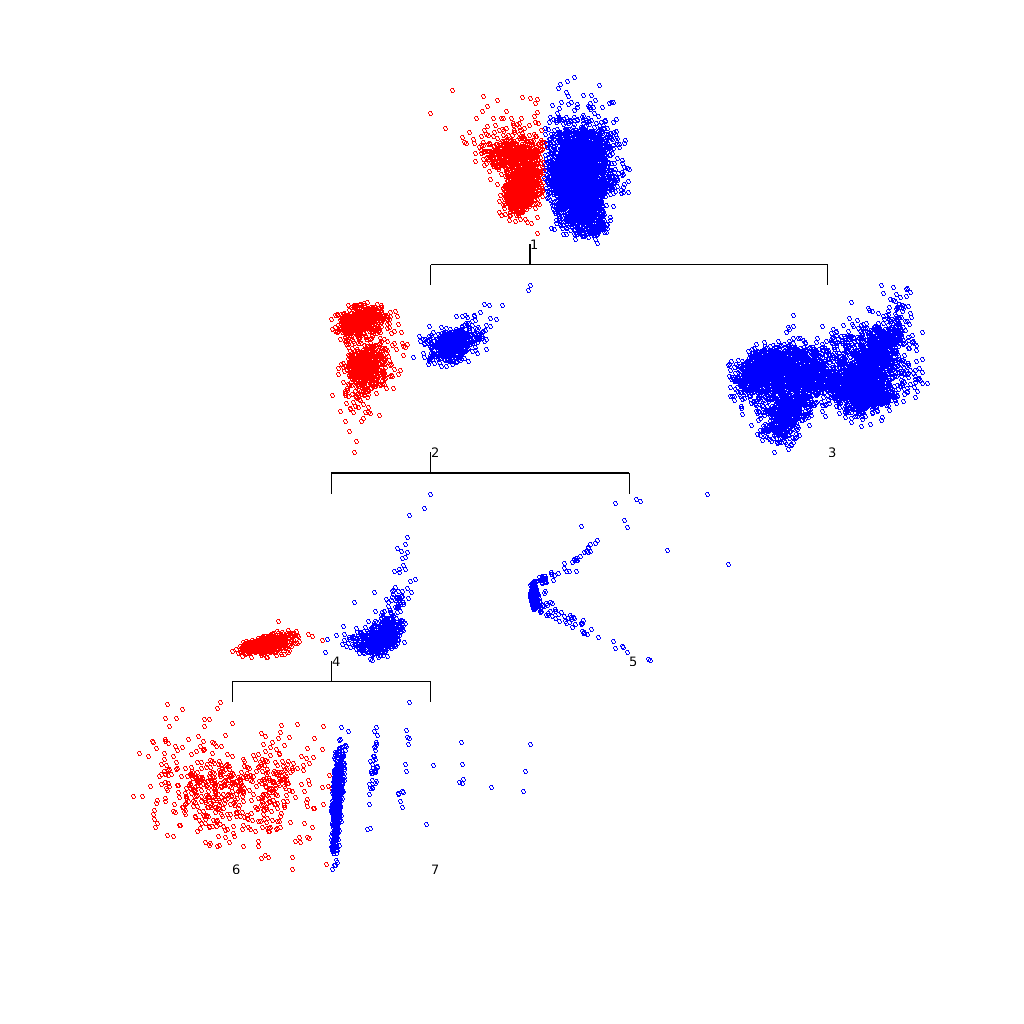
\includegraphics[scale=0.7]{figures/val5.png}} 
%
\end{htmlonly}
%
\caption{Cluster hierarchy after splitting node 2 and its children, and then after pruning node 3. Note
how the numbers of nodes have changed after pruning the tree: node numbers represent the order 
in which nodes are added to the tree}
%
\label{fig:val2}
\end{figure}


Having pruned the tree we next explore whether the cluster at node 3 can be
split more effectively. If we simply apply the {\tt split} function on the
cluster at node 3 we will obtain the same hyperplane as before. The reason for
this is that the {\tt split} function bi-partitions a cluster using the same
arguments that were used when the {\tt ctree} object was first created. 
%
The user can modify this behaviour by specifying optional arguments.
%
The {\tt split} function accepts all the arguments (using
the same syntax) as the divisive hierarchical clustering algorithm
that created the first instance of the {\tt ctree} object.
%
In this example, 
we consider MDHs obtained by initialising the projection vector
at the 2nd and 3rd principal
component. To this end we need to set the {\tt v0} argument.
%
In the code below we also set the {\tt verb} argument to one to enable
the visualisation of the progress of the algorithm.
%
Monitoring the progress of the projection pursuit algorithm we observe that the
most promising MDH is obtained for the initialisation at the third principal
component. Using the default parameter settings the algorithm rejects this solution
because it is outside the default range around the mean of the data.
%
To overcome this we increase the maximum range by setting
{\tt alphamax} to 1.2 (from a default of one). Note in the second sub-figure in Figure~\ref{fig:val3}
that the local minimiser along the projected density is very close
to the boundary of the range of admissible MDHs (evident by
the blue dashed line that illustrates the projection index, Eq.~(\ref{eq:mdh2})).

\begin{verbatim}
>> % Prune tree at node 3
>> t1 = prune(t1,3);
>> % Consider alternative parameter settings for PP algorithm:
>> % initialise at 2nd PC
>> split(t1,3,'v0',@(x,p)(pcacomp(x,2)), 'verb',1);
>> % initialise at 3rd PC, and increase range of admissible MDHs
>> split(t1,3,'v0',@(x,p)(pcacomp(x,2)), 'alphamax',1.2, 'verb',1);
>> % Update cluster hierarchy
>> t1 = split(t1,3,'v0',@(x,p)(pcacomp(x,2)), 'alphamax',1.2);
\end{verbatim}


\begin{figure}
%
\begin{latexonly}
%
\begin{center}
%\subfigure[Cluster hierarchy]{ 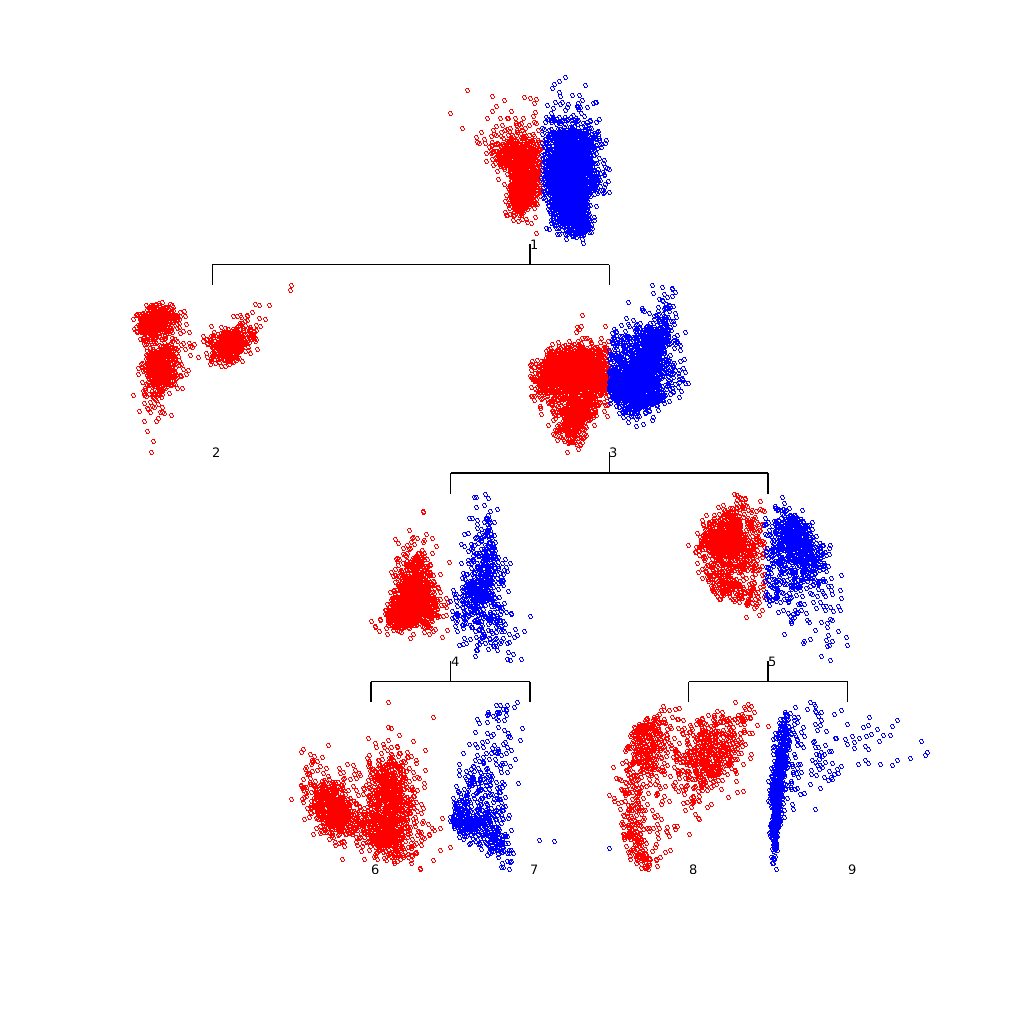
\includegraphics[scale=0.3]{figures/val1.png}}
%
\subfigure[Initialisation at 2nd PC]{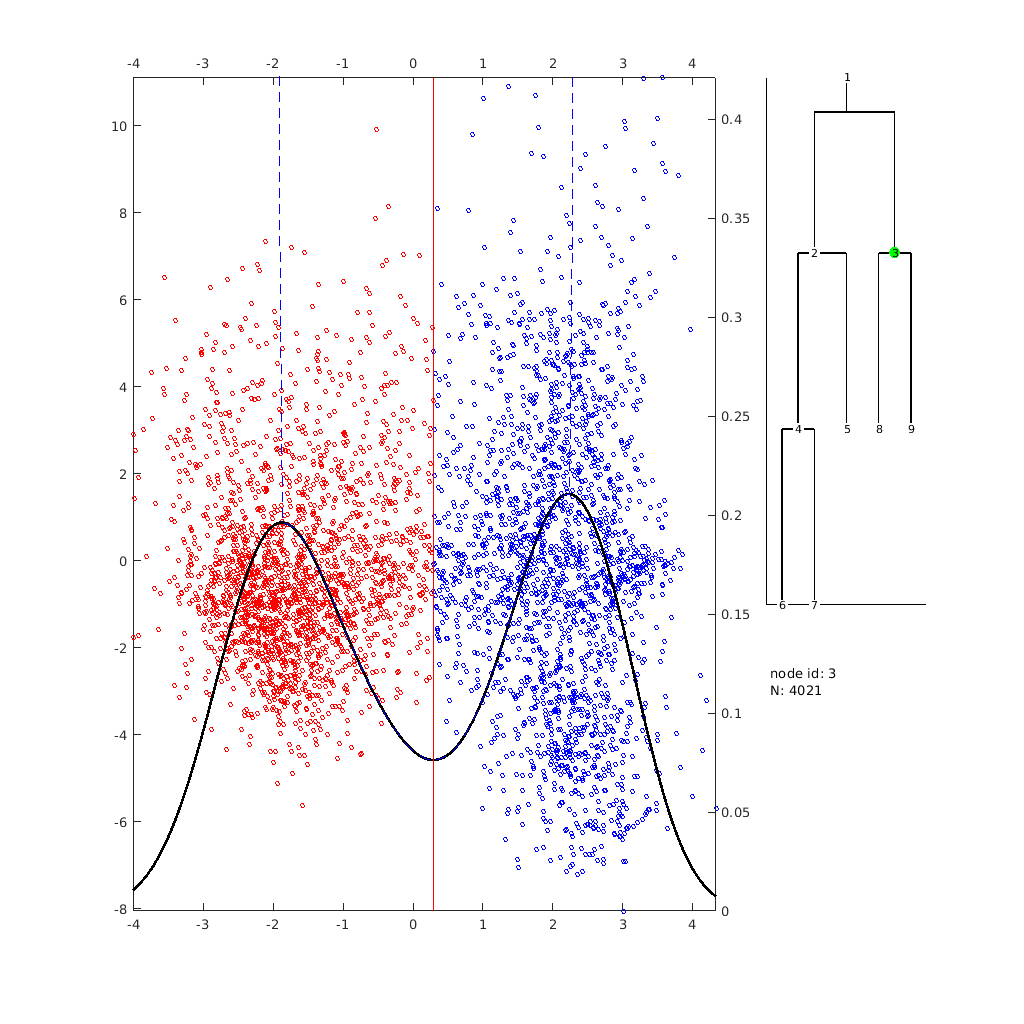
\includegraphics[scale=0.3]{figures/val6.png}} 
%
\subfigure[Initialisation at 3rd PC]{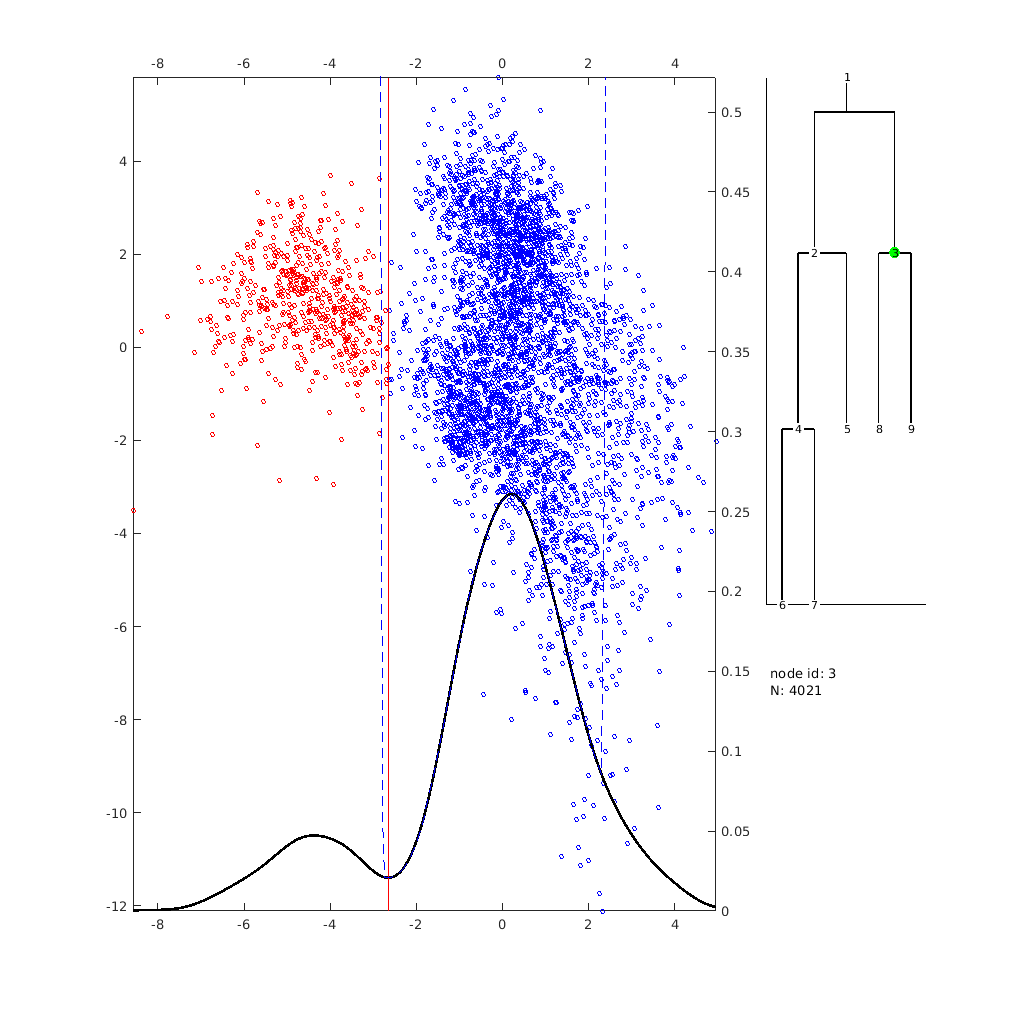
\includegraphics[scale=0.3]{figures/val7.png}} 
%
\end{center}
\end{latexonly}
%
\begin{htmlonly}
%
%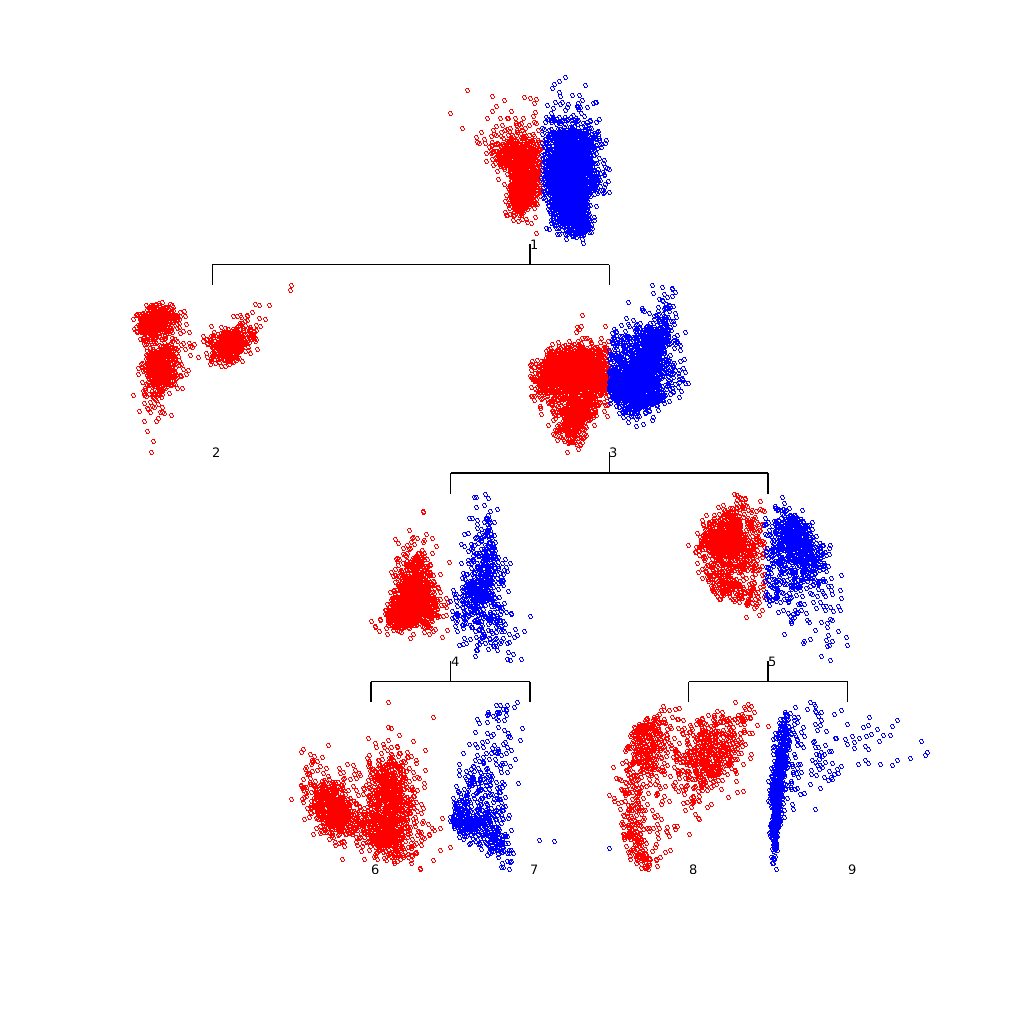
\includegraphics[scale=0.7]{figures/val1.png}} 
%
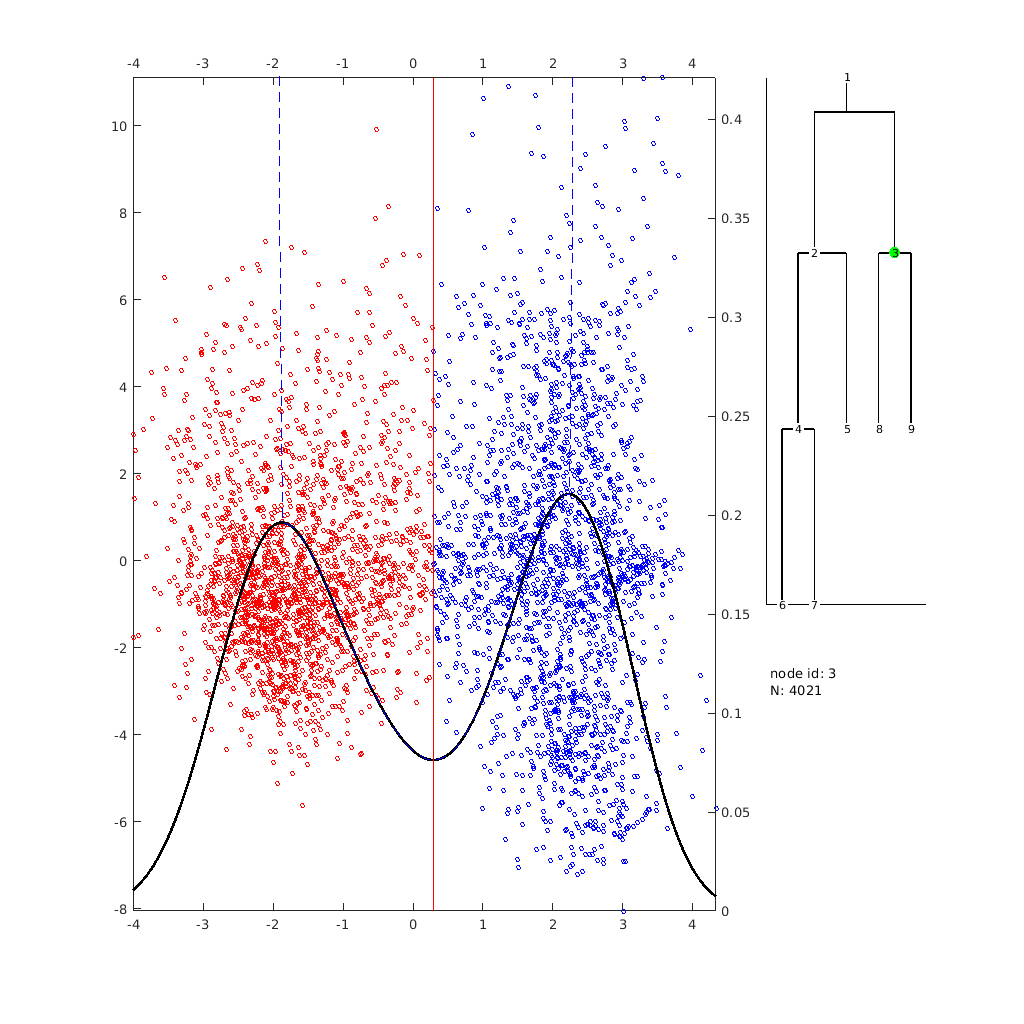
\includegraphics[scale=0.7]{figures/val6.png}} 
%
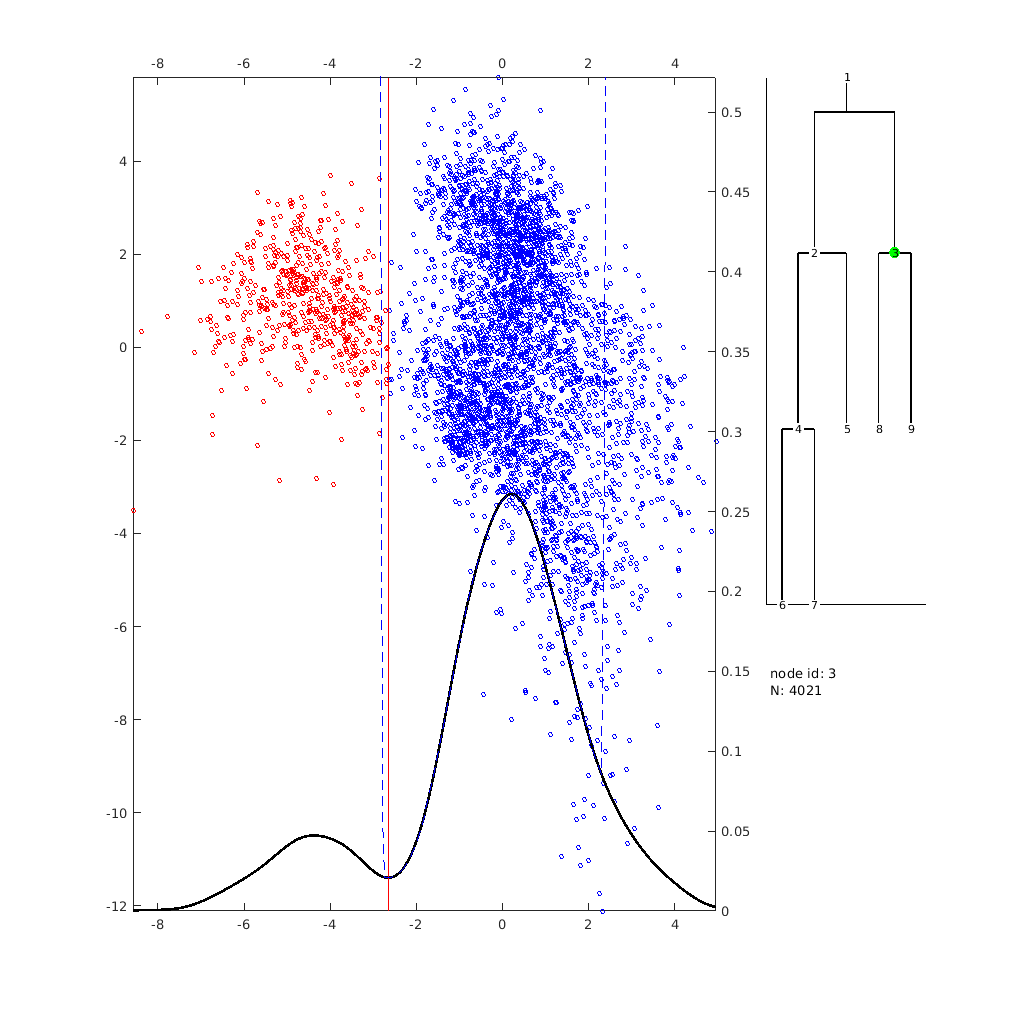
\includegraphics[scale=0.7]{figures/val7.png}} 
%
\end{htmlonly}
%
\caption{Candidate MDH for cluster at node 3 obtained by initialising
at the second and third principal component respectively}
%
\label{fig:val3}
\end{figure}



An inspection of the outcome of the revised clustering model indicates
that both clusters arising from the split of node~3 are likely to contain
more than one clusters. We first split the right child of node 3 and continue
splitting clusters until no cluster exhibits evidence of containing more than 
one dense regions. In the following, the default parameter values for the
projection pursuit algorithm appear appropriate, so they are not modified.
%
For brevity we omit the visualisations of the individual binary partitions
in the following code segment.

\begin{verbatim}
>> % Visualise and then split leaves that 
>> % appear to contain more than one clusters
>> nplot(t1,9);
>> t1 = split(t1,9);
>> nplot(t1,11);
>> t1 = split(t1,11);
>> nplot(t1,12);
>> t1 = split(t1,12);
>> nplot(t1,15);
>> t1 = split(t1,15);
>> nplot(t1,10);
>> t1 = split(t1,10);
>>
>> % Assess performance
>> idx = tree2cluster(t1);
>> cluster_performance(idx, labels)

ans = 

  struct with fields:

      Purity: 0.8484
         NMI: 0.7848
     AdjRand: 0.7280
    Vmeasure: 0.7848

>> % Visualise clustering model
>> plot(t1,labels)
\end{verbatim}


The performance of the final model is higher than that of the model obtained by
{\tt mddc} using the default settings and the correct number of clusters. Indeed
%
The visualisation of the cluster hierarchy in Figure~\ref{fig:val4}
also verifies that the clustering model is appropriate for this dataset.


\begin{figure}
%
\begin{latexonly}
%
\begin{center}
%\subfigure[Cluster hierarchy]{ \includegraphics[scale=0.3]{figures/val1.png}}
%
\includegraphics[scale=0.3]{figures/val8.png}
%
\end{center}
\end{latexonly}
%
\begin{htmlonly}
%
\includegraphics[scale=0.7]{figures/val8.png}} 
%
\end{htmlonly}
%
\caption{Final clustering model}
%
\label{fig:val4}
\end{figure}




\chapter{Extensions}


\section{Maximum Hard Margin Clustering}

Maximum Margin Clustering (MMC)~\cite{XuNLS2004}, extends the maximum margin
principle, which has been very successful in supervised and semi-supervised
classification, to clustering.
%
The MMC problem can be expressed as identifying the binary labelling of $X$
that will maximise the margin of a Support Vector Machine classifier estimated
on the labelled data. MMC corresponds to a nonconvex integer optimisation
problem. 
%
exact methods for this problem are only feasible for very small datasets.
%
MMC algorithms that can handle reasonably sized datasets are not guaranteed
to converge to the global optimum.
%
The minimum density hyperplane (MDH) and the minimum normalised cut hyperplane
(NCUTH) converge to the maximum hard margin hyperplane as the bandwidth
(scaling) parameter is reduced towards zero~\cite{PavlidisHT2016,Hofmeyr2017}. 
%
%Unlike MMC methods that operate on the kernel matrix and are therefore able to
%identify clusters that are not linearly separable, MDH and NCUTH operate on
%the original Euclidean space and can identify only linearly separable
%clusters.
%
%We discuss the identification this issue in the next section.


We illustrate this using the test set of the optical recognition of handwritten
digits dataset, which is widely used as a benchmark in the MMC literature.
%
One of the most difficult binary classification problems from this dataset is
the separation of digits 3 and~9~\cite[Table IV]{ZhangTK2009}.
%
We standardise the dataset as in all previous examples.
%
In the next example we recursively half the bandwidth parameter
employed by the {\tt mdh} function until the vector that is orthogonal to the
estimated MDH converges. 
%
At each iteration the projection vector is initialised to the 
vector that is orthogonal to the previously
identified optimal MDH. 

\begin{verbatim}
>> load('datasets/optidigitsTest.mat');
>> % Observations corresponding to digits 3 and 9
>> index = find(labels==3 | labels==9);
>> % Standardise data matrix
>> X = normalise(X(index,:), 1);
>> labels = labels(index);
>> 
>> % Estimate MDH with default bandwidth
>> [~,hp0] = mdh(X);
>> 
>> hp = hp0;
>> % Value of alpha for which MDH is obtained
>> a = hp.params.alpha;
>> v0 = zeros(size(X,2),1);
>> while abs(hp.v' * v0) < 1-1.e-6,
>> 	% obtain initial projection vector and bandwidth parameter
>> 	v0 = hp.v;
>> 	h = 0.5*hp.params.bandwidth;
>> 	[idx,hp]= mdh(X,'v0',v0,'alphamin',a,'alphamax',a,'bandwidth',h);
>> end
>> plot(hp0,X);
>> plot(hp,X);
>> er = 1 - purity(idx, labels(index))

er =

    0.0248

\end{verbatim}


\begin{figure}
%
\begin{latexonly}
%
\begin{center}
%
\subfigure[Initial MDH]{\includegraphics[scale=0.3]{figures/mm1.png}} 
%
\subfigure[Final MDH]{\includegraphics[scale=0.3]{figures/mm2.png}} 
%
\end{center}
\end{latexonly}
%
\begin{htmlonly}
%
\includegraphics[scale=0.7]{figures/mm1.png}} 
%
\includegraphics[scale=0.7]{figures/mm2.png}} 
%
\end{htmlonly}
%
\caption{Large hard margin separators obtained by recursively applying {\tt mdh} 
for decreasing sequence of bandwidths}
%
\label{fig:mmc1}
\end{figure}


The minimum normalised cut hyperplane (NCUTH) also
converges to the maximum hard margin hyperplane
as the scaling parameter $\sigma$
for the Gaussian kernel used to compute pairwise similarities is reduced
towards zero. In the next example we illustrate this using the
{\tt ncuth} function.

\begin{verbatim}
>> % Estimate NCUTH with default bandwidth
>> [idx,hp0] = ncuth(X);
>> plot(hp0,X);
>> 
>> hp = hp0;
>> v0 = 0*hp.v;
>> while abs(hp.v'*v0) < 1-1.e-10,
>> 	v0 = hp.v;
>> 	s = 0.5*hp.params.sigma;
>> 	[id,hp]= ncuth(X,'v0',v0,'sigma',s);
>> end
>> plot(hp0,X);
>> plot(hp,X);
>> er = 1 - purity(id, labels)

er =

    0.0248

\end{verbatim}


\begin{figure}
%
\begin{latexonly}
%
\begin{center}
%
\subfigure[Initial NCUTH]{\includegraphics[scale=0.3]{figures/mm3.png}} 
%
\subfigure[Final NCUTH]{\includegraphics[scale=0.3]{figures/mm4.png}} 
%
\end{center}
\end{latexonly}
%
\begin{htmlonly}
%
\includegraphics[scale=0.7]{figures/mm3.png}} 
%
\includegraphics[scale=0.7]{figures/mm4.png}} 
%
\end{htmlonly}
%
\caption{Large hard margin separators using {\tt ncuth} for a decreasing sequence
of scaling parameters for the Gaussian kernel}
%
\label{fig:mmc2}
\end{figure}


\noindent
%
The large margin hyperplane obtained by both NCUTH and MDH achieve a
substantial improvement over all the methods reported
in~\cite[Table~IV]{ZhangTK2009}. These include the standard clustering
algorithms: $k$-means, kernel $k$-means, normalised cut clustering, as well as
maximum margin clustering methods: generalised maximum margin
clustering~\cite{Valizadegan2006}, and the iterative support vector regression.
NCUTH and MDH also outperform the more recent cutting plane maximum margin
clustering algorithm~\cite{WangZZ2010}. (A MATLAB implementation of the last
method is available from the
\href{https://sites.google.com/site/binzhao02/CPMMC.rar?attredirects=0} {lead
author's personal page}.)



\section{Non-linear clustering with hyperplane separators}\label{sec:kpca}

In this section we illustrate a simple example of using Kernel Principal
Component Analysis (KPCA)~\cite{ScholkopfSM1998} to enable the identification of
non--linearly separable, by hyperplane based methods.
%
KPCA enables us to embed the data in a high-dimensional feature space in which
clusters are linearly separable. Hyperplanes in the feature space correspond to
nonlinear cluster boundaries in the original space.  We illustrate this through
a widely used two dimensional data set containing two clusters, each in the
shape of a half moon, arranged so that they cannot be separated by a
hyperplane~\cite{Jain2005}. 

The next example also illustrates the use of the functions, {\tt kpca} and {\tt
kpca\_predict} included in OPC. Both functions are based on the KPCA
description in~\cite{ScholkopfSM1998} and have the same syntax and default
arguments as the implementation of KPCA in the {\tt R} package {\tt
kernelab}~\cite{kernlab}. The only important difference between {\tt kpca} and
{\tt kpca\_predict} in OPC and {\tt kernlab} is that in OPC the user needs to
specify the kernel matrix as an argument. 


\begin{verbatim}
>> load('datasets/halfmoons.dat');
>> % Hyperplane separator in original space
>> idx1 = ncuth(X);
>>
>> % Select randomly 200 observations to estimate KPCA
>> s = randperm(size(X,1),200);
>> % Compute Kernel matrix for data sample
>> sigma = 6;
>> K = exp(-sigma*squareform(pdist(X(s,:)).^2));
>> % Compute Kernel Principal Components
>> pcv = kpca(K);
>> % Project all feature vectors onto pcv
>> Kp = exp(-sigma*mypdist2(X, X(s,:)).^2);
>> X2 = kpca_predict(K,Kp,pcv);
>>
>> % Hyperplane separator in feature space
>> idx2 = ncuth(X2);
\end{verbatim}

\begin{figure}[h]
%
\begin{latexonly}
%
\begin{center}
%
\subfigure[Hyperplane in original space]{\includegraphics[scale=0.22]{figures/kpca1.png}} \hspace{0.3cm}
%
\subfigure[Hyperplane in feature space]{\includegraphics[scale=0.22]{figures/kpca2.png}} 
%
\end{center}
\end{latexonly}
%
\begin{htmlonly}
%
\includegraphics[scale=0.7]{figures/kpca1.png}} 
%
\includegraphics[scale=0.7]{figures/kpca2.png}} 
%
\end{htmlonly}
%
\caption{Hyperplane separators in the original, Euclidean space and in the kernel
defined feature space}
%
\label{fig:kpca}
\end{figure}




%\clearpage

\chapter{Extending OPC}\label{sec:extend}


The OPC package provides a simple interface for users to create divisive
hierarchical algorithms based on projection pursuit methods for clustering. 
%
The function {\tt gppdc} implements a framework for {\em generic projection
pursuit divisive clustering} algorithms.
%
The {\tt gppdc} returns the cluster assignment {\tt idx}, and a {\tt ctree}
object that represents the cluster hierarchy. The user can interact with
this object in the same way as in all the previous examples.
%
The function requires three mandatory inputs: the data matrix, {\tt X}, the
number of clusters, {\tt k}, and a handle to a function that bi-partitions the
data through projection pursuit clustering, {\tt pphandle}.
%

The handle {\tt pphandle} must be associated to the function that performs
binary partitioning through projection pursuit. This is the only function that
the user needs to specify. The function must have the following syntax:

\begin{center}
{\tt [v,fval,idx] = ppfunc(X,param)}
\end{center}
%
where {\tt X} is the data matrix, and {\tt param} is a structured array, which
%
contains any additional arguments which are required to perform projection pursuit.
%
For example the {\tt param} structure can contain a handle to a function that
determines the initial projection matrix.
%
The output arguments of {\tt ppfunc}
are: the projection matrix, {\tt v}, the value of the projection index,
{\tt fval}, and the binary cluster assignment, {\tt idx}~$\in {1,2}^n$.


The generic projection pursuit divisive clustering function, {\tt gppdc},
accepts three optional input arguments: {\tt param}, {\tt split\_index}, and
{\tt labels}.

\begin{enumerate}

\item {\tt param} is used to specify the structured array that contains
all the necessary parameters for the projection pursuit
algorithm, as well as for the computation of the split index.
%
This structured array is used as
the second input argument to the {\tt pphandle} function handle, and
the third argument of the {\tt split\_index} function (described next).

\item {\tt split\_index} is a handle to a function that takes
as input the projection matrix, {\tt v}, the data matrix, {\tt X}, and a
structured array of parameters ({\tt param}) and returns a scalar. The output
of this function is the value of the splitting index for the cluster containing
the observations in {\tt X}.
%
At each step of {\tt gppdc} the cluster with the highest splitting index is
bi-partitioned.

\item {\tt labels} is used to specify the true cluster assignment. This
information is only used after the clustering model is estimated to compute the
success ratio and the purity at internal and terminal nodes of the tree,
respectively.

\end{enumerate}

The next code snippet specifies a function which can be used as a projection
pursuit function to implement the bisecting $k$-means
algorithm~\cite{SteinbachKK2000}. The function does not require the specification 
of any parameters. The data matrix is the only input argument.
It applies 2-means to identify the two cluster centroids ({\tt C}),
and the assignment of observations to clusters ({\tt idx}).
The projection matrix in this case is the vector connecting the two centroids
(normalised to have unit-length). In~\cite{SteinbachKK2000} it is recommended to
split the cluster with the largest size. The projection index, {\tt fval},
is therefore equal to the number of observations.

\begin{verbatim}
function [v,fval,idx] = bisKmeansPP(X)
	[idx,C,sumd] = kmeans(X,2,'EmptyAction','singleton','Replicates',1);
	v = (C(1,:) - C(2,:))';
	v = v./norm(v,2);;
	fval = size(X,1);
end
\end{verbatim}

\noindent
%
The above function is in the file {\tt bisKmeansPP.m} in the directory {\tt src/generic}.
To perform bisecting $k$-means through OPC using as cluster splitting criterion 
the total scatter we can use the {\tt gppdc} function as:

\begin{verbatim}
>> load('datasets/optidigits.mat');
>> [idx,t] = gppdc(X,10, @(x,p)(bisKmeansPP(x)), 'split_index', @(v,x,p)(total_scatter(x)));
\end{verbatim}

\noindent
%
The user can visualise and modify the cluster hierarchy obtained through {\tt
gppdc} through the functions, {\tt plot}, {\tt nplot}, {\tt prune}, and {\tt
split} discussed extensively in Section~\ref{sec:valid}.  No additional code
needs to be written for this functionality to be available.


%\phantomsection 
%\addcontentsline{toc}{section}{References}
\bibliographystyle{plain}
\bibliography{bibfile}

%\clearpage
%\phantomsection 
%%\addcontentsline{toc}{section}{Function Index}
%\printindex{code}{Function Index}


\end{document}
